% Customizable fields and text areas start with % >> below.
% Lines starting with the comment character (%) are normally removed before release outside the collaboration, but not those comments ending lines

%%%%%%%%%%%%% local definitions %%%%%%%%%%%%%%%%%%%%%


%%%%%%%%%%%%%%%  Title page %%%%%%%%%%%%%%%%%%%%%%%%
\cmsNoteHeader{AN-19-243} % This is over-written in the CMS environment: useful as preprint no. for export versions
% >> Title: please make sure that the non-TeX equivalent is in PDFTitle below for papers. For PASs, PDFTitle can be used with plain TeX.
\title{Search for VBF Higgs bosons decaying to invisible particles at 13 TeV with 2017 and 2018 data}

% >> Authors
%Author is always "The CMS Collaboration" for PAS and papers, so author, etc, below will be ignored in those cases
%For multiple affiliations, create an address entry for the combination
%To mark authors as primary, use the \author* form
\address[inst1]{Boston University (US)}
\author*[inst1]{Alp Akpinar}
\author*[inst1]{Zeynep Demiragli}
\author*[inst1]{Andreas Albert}
\author*[inst1]{Siqi Yuan}

% >> Date
% The date is in yyyy/mm/dd format. Today has been
% redefined to match, but if the date needs to be fixed, please write it in this fashion.
\date{\today}

% >> Abstract
% Abstract processing:
% 1. **DO NOT use \include or \input** to include the abstract: our abstract extractor will not search through other files than this one.
% 2. **DO NOT use %**                  to comment out sections of the abstract: the extractor will still grab those lines (and they won't be comments any longer!).
% 3. For PASs: **DO NOT use CMS tex macros.**...in the abstract: CDS MathJax processor used on the abstract doesn't understand them _and_ will only look within $$. The abstracts for papers are hand formatted so macros are okay.
\abstract{
   This note describes the search for invisible decays of Higgs boson produced with vector boson fusion (VBF). The search is performed using
   a shape-based analysis, using the data collected by CMS at $\sqrt{s} = 13 \ TeV$ in 2017 and 2018, corresponding to integrated luminosities of
   $41.3 fb^{-1}$ and $59.7 fb^{-1}$, respectively.
}

% >> PDF Metadata
% Do not comment out the following hypersetup lines (metadata). They will disappear in NODRAFT mode and are needed by CDS.
% Also: make sure that the values of the metadata items are sensible and are in plain text with the possible exception of the PDFtitle for a PAS. Then you can use pure TeX symbols as if on a typewriter. Examples: $\sqrt{s}=13\TeV$ => $sqrt{s}=$ 13 TeV; 32\fbinv => 32 fb$^{-1}$
% No unescaped comment % characters.
% No curly braces {} except for TeX in the PDFtitle.
\hypersetup{%
pdfauthor={Alp Akpinar, Andreas Albert, Zeynep Demiragli, Siqi Yuan},%
pdftitle={Run-II VBFHinv BU},%
pdfsubject={CMS},%
pdfkeywords={CMS, physics, your topics}}

\maketitle %maketitle comes after all the front information has been supplied
% >> Text
%%%%%%%%%%%%%%%%%%%%%%%%%%%%%%%%  Begin text %%%%%%%%%%%%%%%%%%%%%%%%%%%%%
%% **DO NOT REMOVE THE BIBLIOGRAPHY** which is located before the appendix.
%% You can take the text between here and the bibiliography as an example which you should replace with the actual text of your document.
%% If you include other TeX files, be sure to use "\input{filename}" rather than "\input filename".
%% The latter works for you, but our parser looks for the braces and will break when uploading the document.
%%%%%%%%%%%%%%%
\ifthenelse{\boolean{cms@external}}{\newcommand{\PV}{\ensuremath{V}\xspace}}{\newcommand{\PV}{\ensuremath{\mathrm{V}}\xspace}}
\newcommand{\Zmm}{\ensuremath{\mathrm{Z}\to\mu^+\mu^-}}
\newcommand{\Zee}{\ensuremath{\mathrm{Z}\to e^+e^-}}
\newcommand{\Zll}{\ensuremath{\mathrm{Z}\to\ell\ell}}
\newcommand{\Zvv}{\ensuremath{\mathrm{Z}\to\nu\nu}}
\newcommand{\Wlv}{\ensuremath{\mathrm{W}\to \ell\nu}}
\newcommand{\Wmn}{\ensuremath{\mathrm{W}\to \mu\nu}}
\newcommand{\Wen}{\ensuremath{\mathrm{W}\to e\nu}}
\newcommand{\Zmmjets}{\ensuremath{\mathrm{Z}(\mu\mu)+\textrm{jets}}}
\newcommand{\Zeejets}{\ensuremath{\mathrm{Z}(ee)+\textrm{jets}}}
\newcommand{\Zlljets}{\ensuremath{\mathrm{Z}(\ell\ell)+\textrm{jets}}}
\newcommand{\Zjets}{\ensuremath{\mathrm{Z}+\textrm{jets}}}
\newcommand{\Wjets}{\ensuremath{\mathrm{W}+\textrm{jets}}}
\newcommand{\Zvvjets}{\ensuremath{\mathrm{Z}(\nu\nu)+\textrm{jets}}}
\newcommand{\Wlvjets}{\ensuremath{\mathrm{W}(\ell\nu)+\textrm{jets}}}
\newcommand{\Wmvjets}{\ensuremath{\mathrm{W}(\mu\nu)+\textrm{jets}}}
\newcommand{\Wmnjets}{\ensuremath{\mathrm{W}(\mu\nu)+\textrm{jets}}}
\newcommand{\Wevjets}{\ensuremath{\mathrm{W}(e\nu)+\textrm{jets}}}
\newcommand{\Wenjets}{\ensuremath{\mathrm{W}(e\nu)+\textrm{jets}}}
\newcommand{\phojets}{\ensuremath{\gamma+\textrm{jets}}}
\newcommand{\brhiggs}{\ensuremath{0.62}}
\newcommand{\higgsbr}{\ensuremath{0.62}}
\newcommand{\higgsbrobs}{\ensuremath{0.53}}
\newcommand{\cchiggsbr}{\ensuremath{0.92}}
\newcommand{\Et}{\ensuremath{E_\mathrm{T}}}
\newcommand{\mt}{\ensuremath{M_\mathrm{T}}}
\newcommand{\met}{\ensuremath{\Et^{\mathrm{miss}}}}
\newcommand{\metcalo}{\ensuremath{E_\mathrm{T \ calo}}^{\mathrm{miss}}}
\newcommand{\metpf}{\ensuremath{E_\mathrm{T \ PF}}^{\mathrm{miss}}}
\newcommand{\Ht}{\ensuremath{H_\mathrm{T}}}
\newcommand{\sieie}{\ensuremath{\sigma_{i\eta i\eta}} }
\newcommand{\vmet}{\ensuremath{\vec{E}_\mathrm{T}}^{\text{miss}}\xspace}
\newcommand{\numberthis}{\addtocounter{equation}{1}\tag{\theequation}}
\newcommand{\mettrig}{\ensuremath{E_{\mathrm{T, trig}}^{\mathrm{miss}}}}
\newcommand{\mhttrig}{\ensuremath{H_{\mathrm{T, trig}}^{\mathrm{miss}}}}
\newcommand{\brhinv}{\ensuremath{\mathcal{B}(\mathrm{H}\rightarrow \mathrm{inv})}}
\newcommand{\ptvecjet}{\ensuremath{{\vec p}_{\mathrm{T}}^{\kern1pt\text{jet}}}\xspace}
\newcommand{\qt}{\ensuremath{{q}_{\rm T}}\xspace}
\newcommand{\vqt}{\ensuremath{\vec{q}_{\rm T}}\xspace}
\newcommand{\vut}{\ensuremath{\vec{u}_{\rm T}}\xspace}
\newcommand{\vpt}{\ensuremath{\vec{p}_{\rm T}}\xspace}

\newcommand{\hatqt}{\ensuremath{{\hat q}_{\rm T}}\xspace}
\newcommand{\hatut}{\ensuremath{{\hat u}_{\rm T}}\xspace}
\newcommand{\hatpt}{\ensuremath{{\hat p}_{\rm T}^\ell}\xspace}
\newcommand{\bisec}{\ensuremath{{\hat b}}\xspace}
\newcommand{\upar}{\ensuremath{u_\Vert}\xspace}
\newcommand{\upara}{\ensuremath{u_\Vert}\xspace}
\newcommand{\uperp}{\ensuremath{u_\perp}\xspace}
\newcommand{\redupara}{\ensuremath{u_\Vert + \qt}\xspace}
\newcommand{\reso}[1]{\ensuremath{ \sigma(#1) }\xspace}
\newcommand{\resp}{\ensuremath{- \langle \upar \rangle / \qt}\xspace}

\newcommand{\ptmisstrig}{\ensuremath{p_{\mathrm{T, trig}}^{\mathrm{miss}}}}
\newcommand{\ptmiss}{\ensuremath{p_{\mathrm{T}}^{\mathrm{miss}}}}
\newcommand{\htmiss}{\ensuremath{H_{\mathrm{T}}^{\mathrm{miss}}}}
\newcommand{\pthat}{\ensuremath{\hat{p}_{\mathrm{T}}}\xspace}
\newcommand{\ptv}{\ensuremath{p_{\mathrm{T},V}}\xspace}

\newcommand{\detajj}{\Delta \eta_{jj}}
\newcommand{\dphijj}{\Delta \phi_{jj}}
\newcommand{\mjj}{M_{jj}}
\tableofcontents
\newpage
\section{Introduction} \label{section:introduction}

This analysis note describes a search for Higgs boson produced by vector boson fusion (VBF), 
decaying into invisible particles. The signature of such a final state will be two seperated jets 
and an imbalance in $\vpt$ due to the undetected particles. Two seperated jets are the result of the 
hadronization of two final state quarks emerging from the VBF process.

This analysis makes use of data collected with the CMS detector in proton-proton (pp) collisions in 2017 
and 2018 at $\sqrt{s}=13\TeV$, corresponding to an integrated luminosity of 41.3 $\fbinv$ and 59.7 $\fbinv$, 
respectively. 

The analysis strategy is similar to that of 2016 VBF analysis, with several improvements. One of the major 
improvements in this analysis is the addition of a new control region: photon control region. % can add info about the positive sides of photon CR here
% EWK k-factor updates (2D k-factors)?
% More improvements in the analysis (VBF trigger for signal extraction in lower recoil?) 

\section{Samples} \label{sec:samples}

The analysis described in this note is performed using data collected in 2017 by
CMS at 13 TeV and corresponds to an integrated luminosity of 41.5 fb$^{-1}$.
The MC simulation samples for the background processes
have been produced in the \texttt{Fall17} and \texttt{Autumn18} campaigns. Further details
are given in the following sub-sections.

\subsection{Data Samples}

The datasets listed in Tab.~\ref{tab:DataSamples} are used to
select events in the signal and the control regions, and to perform measurments on physics objects
used in the analysis (e.g. trigger turn-ons).

\begin{table}[ht!]
    \centering
    \small
    \def\arraystretch{1.5}
    \caption{List of datasets used to select events in the signal and control regions. Datasets for both years correspond to the \texttt{Nano1June2019} campaign, otherwise known as \texttt{v5}. For the 2017 data, the \texttt{31Mar2018} reconstruction is used for all periods. For 2018 data, the \texttt{17Sep2018} reconstruction is used for runs A to C, and the \texttt{22Jan2019} reconstruction is used for run D.}
    \begin{tabular}{l l p{8cm}}
        \hline
        \hline
        Year                  & Dataset name                       & Events selected for                                                     \\
        \hline
        \hline
        both                  & {/MET/Run201*/NANOAOD}             & Signal , single muon, double muon control regions                 \\\hline
        \multirow{2}{*}{2017} & {/SingleElectron/Run2017*/NANOAOD} & Single electron, double electron control regions                        \\
                              & {/SinglePhoton/Run2017*/NANOAOD}   & Single photon control region                                            \\\hline
        2018                  & {/EGamma/Run2018*/NANOAOD}         & Single electron, double electron control, single photon control regions \\
        \hline
        \hline
    \end{tabular}

    \label{tab:DataSamples}
\end{table}

Events for the signal region are collected using a set of dedicated
triggers designed to select events with large \ptmiss and large \mht based on
the online particle flow (PF) algorithm. In these dedicated trigger algorithms,
identified PF muons are removed from the event before the
\ptmiss~and the \mht~objects are calculated. With this definition,
the signal trigger paths can also be used to select single and double muon events for the W and Z control regions, respectively.

Electron events for the W and Z regions are selected using a single electron trigger.
To ensure the trigger efficiency also for high-\pt electrons, the single electron trigger is used in combination with
a single photon trigger~\cite{CMS-EGM-TWIKI-HLT}. The same photon trigger is used to select events for the photon control region.

The full list of triggers used, along with the L1 seeds and the associated primary datasets are shown in Table~\ref{tab:triggers}.

\begin{table}[h]
    \centering
    \def\arraystretch{1.5}

    \small
    \caption{HLT paths and the associated L1 seeds used in the analysis for the 2017 and 2018 datasets. The HLT paths ending in ``\_HT60'' are backup triggers introduced  to mitigate noise rate problems in 2017. Their inclusion is not strictly necessary for 2018, but is done for consistency.}

    \footnotesize
    \begin{tabular}{l l c c}
        \hline\hline
        Year                   & HLT path                                                  & L1 seed                         & Primary dataset               \\\hline\hline
        \multirow{5}{*}{2017}  & HLT\_PFMETNoMu120\_PFMHTNoMu120\_IDTight                  & \texttt{L1\_ETMHF70}            & MET                           \\
                               & HLT\_PFMETNoMu120\_PFMHTNoMu120\_IDTight\_PFHT60          & \texttt{L1\_ETMHF80\_HTT60er }  & MET                           \\\cline{2-4}
                               & HLT\_Ele35\_WPTight\_Gsf                                  & \texttt{L1\_SingleEG24}         & SingleElectron                \\\cline{2-4}
                               & \multirow{3}{*}{HLT\_Photon200}                           & \texttt{L1\_SingleEG30}         & \multirow{3}{*}{SinglePhoton} \\
                               &                                                           & \texttt{L1\_SingleJet170}       &                               \\
                               &                                                           & \texttt{L1\_SingleTau100er2p1}  &                               \\\hline\hline

        \multirow{11}{*}{2018} & \multirow{2}{*}{HLT\_PFMETNoMu120\_PFMHTNoMu120\_IDTight} & \texttt{L1\_ETMHF100}           & \multirow{3}{*}{MET}          \\
                               &                                                           & \texttt{L1\_ETM150}             &                               \\
                               & HLT\_PFMETNoMu120\_PFMHTNoMu120\_IDTight\_PFHT60          & \texttt{L1\_ETMHF90\_HTT60er}   &                               \\\cline{2-4}
                               & \multirow{3}{*}{HLT\_Ele32\_WPTight\_Gsf}                 & \texttt{L1\_SingleIsoEG24er2p1} & \multirow{3}{*}{EGamma}       \\
                               &                                                           & \texttt{L1\_SingleEG26er2p5}    &                               \\
                               &                                                           & \texttt{L1\_SingleEG60}         &                               \\\cline{2-4}

                               & \multirow{5}{*}{HLT\_Photon200}                           & \texttt{L1\_SingleEG34er2p5}    & \multirow{5}{*}{EGamma}       \\
                               &                                                           & \texttt{L1\_SingleJet160er2p5}  &                               \\
                               &                                                           & \texttt{L1\_SingleJet180}       &                               \\
                               &                                                           & \texttt{L1\_SingleTau120er2p1}  &                               \\
                               &                                                           & \texttt{L1\_SingleEG60}         &                               \\\hline

        \hline\hline %--------------------------------------------------------------------------------------------------------------------------      \
    \end{tabular}

    \label{tab:triggers}
\end{table}

\subsection{Background Samples}


Simulation datasets for the background processes are listed in
Table~\ref{tab:BackgroundSamples} and~\ref{tab:BackgroundSamples_2}.
There are several Standard Model processes that pose as backgrounds to the VBF $H_{inv}$ signal, experimental signature of the
final state being two jets with large rapidity seperation and invariant mass, along with \ptmiss.
These processes are as follows:

\begin{description}
\item[\Zvvjets]: This process yields the largest irreducible background in the analysis, consisting of a Z boson and 2 or more
jets coming from either QCD or EWK vertices. Simulated samples for this background have been produced at leading
order (LO) in QCD using the aMC@NLO generator in several bins of \Ht for the QCD case, and in one inclusive sample for the EWK case.

\item[\Wjets]: This process is the second largest source of background in this analysis, consisting of a W boson and 2 or more
jets coming from either QCD or EWK vertices. The contribution of this background can be reduced by rejecting events with
charged lepton candidates (electron/muon/tau).
However, this process becomes irreducible in the case where the charged leptons are outside of the detector acceptance.
Simulation samples for this background have been generated at LO in QCD using the aMC@NLO generator in several bins \Ht for the QCD case, and in once inclusive sample for the EWK case.

\item[\Zlljets]: This process mimics signal-like events in the case where the leptons coming from the Z boson decay are
not reconstructed. As in the case of \Wlv, the contribution of this background is reduced by rejecting events with charged leptons.
Simulation samples for this process have been generated at LO in QCD using the aMC@NLO generator in bins of \Ht for the QCD case, and in once inclusive sample for the EWK case.

\item[Top:] Top-quark decays (both \ttbar and single top) also contribute background events to this analysis.
In these processes, the W boson produced in a top-quark decay further decays leptonically, which produces genuine \ptmiss in the event.
Next-to-leading order (NLO) \ttbar simulation samples have been produced with the aMC@NLO generator with two additional partons in the matrix element.
Single-top events have been generated with the Powheg generator at NLO in QCD with one additional matrix element parton.

\item[Dibosons:] Decays of diboson pairs (WW, WZ, ZZ) also constitute background processes.
Typically, one of the bosons decays leptonically (\Wlv,\Zvv) while the other boson decays hadronically, thus producing jets and \ptmiss~in the final state.
Simulated samples for WW, WZ and ZZ production have been generated at LO with Pythia~8.

\item[QCD Multijet:] QCD multijet events typically do not have large genuine \ptmiss.
However, given the large cross section with which these events are produced, even a small fraction of events with
jet mismeasurement results in a non-zero contribution of this process as background in the analysis.
Simulated QCD samples have been generated at LO in QCD using the MadGraph generator in several bins of \Ht.

\end{description}

\begin{table}[ht!]
\centering
\scriptsize
    \def\arraystretch{1.3}
\begin{tabular}{l|r|c}
\hline
\hline
Dataset name                                                                  &  Cross section (pb)          & Order in QCD \\
\hline
\hline
WJetsToLNu\_HT-70To100\_TuneCP5\_13TeV-madgraphMLM-pythia8                        &   1296         & LO  \\
WJetsToLNu\_HT-100To200\_TuneCP5\_13TeV-madgraphMLM-pythia8                       &   1392         & LO  \\
WJetsToLNu\_HT-200To400\_TuneCP5\_13TeV-madgraphMLM-pythia8                       &    410.2       & LO  \\
WJetsToLNu\_HT-400To600\_TuneCP5\_13TeV-madgraphMLM-pythia8                       &     57.95      & LO  \\
WJetsToLNu\_HT-600To800\_TuneCP5\_13TeV-madgraphMLM-pythia8                       &     12.98      & LO  \\
WJetsToLNu\_HT-800To1200\_TuneCP5\_13TeV-madgraphMLM-pythia8                      &      5.39      & LO  \\
WJetsToLNu\_HT-1200To2500\_TuneCP5\_13TeV-madgraphMLM-pythia8                     &      1.08      & LO  \\
WJetsToLNu\_HT-2500ToInf\_TuneCP5\_13TeV-madgraphMLM-pythia8                      &      0.008098  & LO  \\
\hline
ZJetsToNuNu\_HT-100To200\_13TeV-madgraph                                         &    305.3       & LO  \\
ZJetsToNuNu\_HT-200To400\_13TeV-madgraph                                         &     91.86      & LO  \\
ZJetsToNuNu\_HT-400To600\_13TeV-madgraph                                         &     13.13      & LO  \\
ZJetsToNuNu\_HT-600To800\_13TeV-madgraph                                         &      3.242     & LO  \\
ZJetsToNuNu\_HT-800To1200\_13TeV-madgraph                                        &      1.501     & LO  \\
ZJetsToNuNu\_HT-1200To2500\_13TeV-madgraph                                       &      0.3431    & LO  \\
ZJetsToNuNu\_HT-2500ToInf\_13TeV-madgraph                                        &      0.005146  & LO  \\
\hline
DYJetsToLL\_M-50\_HT-70to100\_TuneCP5\_13TeV-madgraphMLM-pythia8                   &    146.9       & LO  \\
DYJetsToLL\_M-50\_HT-100to200\_TuneCP5\_13TeV-madgraphMLM-pythia8                  &    160.9       & LO  \\
DYJetsToLL\_M-50\_HT-200to400\_TuneCP5\_13TeV-madgraphMLM-pythia8                  &     48.68      & LO  \\
DYJetsToLL\_M-50\_HT-400to600\_TuneCP5\_13TeV-madgraphMLM-pythia8                  &      6.998     & LO  \\
DYJetsToLL\_M-50\_HT-600to800\_TuneCP5\_13TeV-madgraphMLM-pythia8                  &      1.745     & LO  \\
DYJetsToLL\_M-50\_HT-800to1200\_TuneCP5\_13TeV-madgraphMLM-pythia8                 &      0.8077    & LO  \\
DYJetsToLL\_M-50\_HT-1200to2500\_TuneCP5\_13TeV-madgraphMLM-pythia8                &      0.1923    & LO  \\
DYJetsToLL\_M-50\_HT-2500toInf\_TuneCP5\_13TeV-madgraphMLM-pythia8                 &      0.003477  & LO  \\
\hline
GJets\_HT-40To100\_TuneCP5\_13TeV-madgraphMLM-pythia8                             &  18640         & LO  \\
GJets\_HT-100To200\_TuneCP5\_13TeV-madgraphMLM-pythia8                            &   8641         & LO  \\
GJets\_HT-200To400\_TuneCP5\_13TeV-madgraphMLM-pythia8                            &   2196         & LO  \\
GJets\_HT-400To600\_TuneCP5\_13TeV-madgraphMLM-pythia8                            &    258.4       & LO  \\
GJets\_HT-600ToInf\_TuneCP5\_13TeV-madgraphMLM-pythia8                            &     85.23      & LO  \\
\hline
\hline
\end{tabular}
\caption{Simulated datasets for the modelling of single electroweak boson backgrounds.
All datasets are accessed at the NanoAOD data tier from the \texttt{v5} campaign, also known as \texttt{1Jun19}.}
\label{tab:BackgroundSamples}
\end{table}



\begin{table}[ht!]
    \centering
    \scriptsize
        \def\arraystretch{1.3}
    \begin{tabular}{l|r|c}
    \hline
    \hline
    Data set name                                                                  &  Cross section (pb)          & Order in QCD \\
    \hline
    \hline

    EWKWMinus2Jets\_WToLNu\_M-50\_TuneCP5\_13TeV-madgraph-pythia8                      &     20.35      & LO  \\
    EWKWPlus2Jets\_WToLNu\_M-50\_TuneCP5\_13TeV-madgraph-pythia8                       &     25.81      & LO  \\
    EWKZ2Jets\_ZToLL\_M-50\_TuneCP5\_13TeV-madgraph-pythia8                            &      4.321     & LO  \\
    EWKZ2Jets\_ZToNuNu\_TuneCP5\_13TeV-madgraph-pythia8                               &     10.04      & LO  \\
    AJJ\_EWK\_TuneCP5\_13TeV\_amcatnlo-pythia8                                         &      6.096     & NLO \\
    GJets\_Mjj-500\_SM\_5f\_TuneCP5\_EWK\_13TeV-madgraph-pythia8                         &      4.937     & LO  \\
    GJets\_SM\_5f\_TuneCP5\_EWK\_13TeV-madgraph-pythia8                                 &     32.91      & LO  \\

    \hline
    TTJets\_TuneCP5\_13TeV-amcatnloFXFX-pythia8                                      &    831.76      & NLO \\
    \hline
    ST\_t-channel\_top\_4f\_inclusiveDecays\_TuneCP5\_13TeV-powhegV2-madspin-pythia8     &    137.458     & NLO \\

    ST\_t-channel\_antitop\_4f\_inclusiveDecays\_TuneCP5\_13TeV-powhegV2-madspin-pythia8 &     83.0066    & NLO \\
    ST\_tW\_top\_5f\_inclusiveDecays\_TuneCP5\_*\_13TeV-powheg-pythia8                      &     35.85      & NLO \\
    ST\_tW\_antitop\_5f\_inclusiveDecays\_TuneCP5\_*\_13TeV-powheg-pythia8        &     35.85      & NLO \\
    \hline
    WW\_TuneCP5\_13TeV-pythia8                                                       &     75.91      & LO  \\
    WZ\_TuneCP5\_13TeV-pythia8                                                       &     27.56      & LO  \\
    ZZ\_TuneCP5\_13TeV-pythia8                                                       &     12.14      & LO  \\
    \hline
    QCD\_HT1000to1500\_TuneCP5\_13TeV-madgraph-pythia8                                &   1095         & LO  \\
    QCD\_HT1000to1500\_TuneCP5\_13TeV-madgraph-pythia8                                &   1095         & LO  \\
    QCD\_HT100to200\_TuneCP5\_13TeV-madgraph-pythia8                                  &      2.369e+07 & LO  \\
    QCD\_HT1500to2000\_TuneCP5\_13TeV-madgraph-pythia8                                &     99.27      & LO  \\
    QCD\_HT2000toInf\_TuneCP5\_13TeV-madgraph-pythia8                                 &     20.25      & LO  \\
    QCD\_HT200to300\_TuneCP5\_13TeV-madgraph-pythia8                                  &      1.554e+06 & LO  \\
    QCD\_HT300to500\_TuneCP5\_13TeV-madgraph-pythia8                                  & 324300         & LO  \\
    QCD\_HT300to500\_TuneCP5\_13TeV-madgraph-pythia8                                  & 324300         & LO  \\
    QCD\_HT500to700\_TuneCP5\_13TeV-madgraph-pythia8                                  &  29990         & LO  \\
    QCD\_HT50to100\_TuneCP5\_13TeV-madgraphMLM-pythia8                                &      1.85e+08  & LO  \\
    QCD\_HT700to1000\_TuneCP5\_13TeV-madgraph-pythia8                                 &   6374         & LO  \\
    QCD\_HT700to1000\_TuneCP5\_13TeV-madgraph-pythia8                                 &   6374         & LO  \\

    \hline
    \hline
    \end{tabular}
    \caption{Simulated datasets for the modelling of EWK V production and other processes. All datasets are accessed at the NanoAOD data tier from the \texttt{v5} campaign, also known as \texttt{1Jun19}.}
    \label{tab:BackgroundSamples_2}
\end{table}
The MC samples produced using \MGvATNLO, and \POWHEG
generators are interfaced with \PYTHIA using the CP5 tune~\cite{Sirunyan:2019dfx}
for the fragmentation, hadronization, and underlying event description.
In the case of the \MGvATNLO samples, jets from the matrix element calculations
are matched to the parton shower description following the MLM~\cite{Mangano:2006rw} (FxFx~\cite{Frederix:2012ps})
prescription to match jets from matrix element calculations and parton shower description for LO (NLO) samples.
The NNPDF 3.1 NNLO~\cite{Ball:2017nwa}
parton distribution functions (PDFs) are used in all generated samples.
The propagation of all final-state particles through the CMS detector
is simulated with the \GEANT4 software~\cite{Agostinelli:2002hh}.
The simulated events include the effects of pileup, with the multiplicity of reconstructed primary
vertices matching that in data. The average number of pileup interactions per proton bunch crossing
is found to be 32 for both the 2017 and 2018 data samples used in this analysis (assuming a total inelastic proton-proton cross-section).

\subsection{Signal simulation samples}

{\color{red} In this section we should add description of the models, feynman diagrams, important model parameters}

{\color{red} {\bf DMSimp Models}}

{\color{red} {\bf t-channel Model}}

{\color{red} {\bf ADD Model}}

{\color{red} {\bf Leptoquark Model}}

{\color{red} {\bf Higgs Invisible Model}}

\section{Trigger} 
\label{sec:trigger}

The data used in this analysis is collected using triggers that are designed to collect events with high $\ptmiss$ and $\htmiss$. 
These triggers rely on the online version of the Particle Flow algorithm. While calculating $\ptmiss$ and $\htmiss$, identified
Particle Flow muons are removed from the event. Therefore, using the same triggers, one can also select dimuon (Z \rightarrow \mu \mu) 
and single muon (W \rightarrow \mu \nu) events.

The remaining control regions include dielectron (Z \rightarrow ee) and single electron (W \rightarrow e\nu) regions. In these two control
regions, events are selected using the Single Electron trigger. The full list of triggers used in this analysis are given in 
Tab.~\ref{tab:triggers}.

\begin{table}[ht!]
    \centering
    \small
    \def\arraystretch{1.5}
    \caption{HLT paths, and the associated L1 seeds being used in the analysis.}
    \begin{tabular}{l l c}
        \hline
        \hline
                                &                                               \\
        HLT Path                & L1 Seed                   & Primary Dataset   \\
        % Complete the table
        
    \end{tabular}
    
\end{table}

\subsection{Overview of $\met$ triggers}

The $\ptmiss$ and $\htmiss$ based triggers are designed to maximize the signal acceptance. These triggers are seeded at L1 level using
a logical OR of available ETM based seeds. % Add more info about the L1 seeds here

% More info to be added here

\subsection{Efficiency turn-on curves}

The performance of $\ptmiss + \htmiss$ based triggers is measured by using both single muon and double muon events, i.e. sample enriched in
$W \rightarrow \mu\nu$ and $Z \rightarrow \mu\mu$ decays, respectively. The measurement is performed by using both data and MC samples 
for 2017 and 2018, seperately.

$W \rightarrow \mu\nu$ events are selected from Single Muon dataset and WJetsToLNu MC sample. % might add more info about MC sample
The muon must must pass the tight ID requirement. In addition, the transverse mass of the muon must not exceed $160 \ GeV$. 
$Z \rightarrow \mu\mu$ events are selected from Single Muon dataset and ZJetsToLL MC sample. % might add more info about MC sample
For this category of events, there must be at least one muon that is passing the tight ID requirement, and there must be exactly 
2 loose muons. In addition to these requirements, these two muons are required to have opposite charge and have an invariant mass 
consistent with the $Z$ boson, $60 < m_{\mu\mu} < 120 \ GeV$.

In both single muon and double muon events, additional requirements are also imposed. There should be no additional leptons or photons and
b-jets identified in the event. In addition, there must be at least two jets in the event, and the leading two jets must have $\pt$ higher
than $80 \ GeV$ and $40 \ GeV$, respectively. Finally, the two leading jets must satisty $\detajj > 1.0$ and $\dphijj < 1.5$.

To understand the dependence of the turn-on curves on the two leading jets, we measured the efficiency in three different categories:

\begin{itemize}
    \item Two central VBF jets: Leading two jets both satisfying $|\eta| \leq 2.4$
    \item Two forward VBF jets: Leading two jets both satisfying $|\eta| > 2.4$
    \item One central and one forward VBF jet: One of the leading jets is central with $|\eta| \leq 2.4$ and the other jet in the pair is forward 
    with $|\eta| > 2.4$
\end{itemize}

In these three categories, efficiencies are measured as a function of $\mjj$ and recoil, using both data and MC samples for 2017 and 2018,
seperately. Figs.~\ref{fig:eff_mjj_2017_1m}, \ref{fig:eff_mjj_2018_1m}, \ref{fig:eff_recoil_2017_1m} and \ref{fig:eff_recoil_2018_1m} show 
the results obtained from single muon events, whereas Figs.~\ref{fig:eff_mjj_2017_2m}, \ref{fig:eff_mjj_2018_2m}, 
\ref{fig:eff_recoil_2017_2m} and \ref{fig:eff_recoil_2018_2m} show the results obtained from double moun events.

Fig.~\ref{fig:eff_mjj_2017_1m} shows the efficiencies as a function of $\mjj$ in data and MC for the three categories in 2017, 
whereas Fig.~\ref{fig:eff_mjj_2018_1m} shows the efficiencies as a function of $\mjj$ in data and MC for the three categories in 2018. 
Fig.~\ref{fig:eff_recoil_2017_1m} shows the efficiency turn-on curves as a function of recoil in data and MC for the three categories, 
for 2017 samples, whereas Fig.~\ref{fig:eff_recoil_2018_1m} shows the efficiency turn-on curves as a function of recoil in data and MC 
for the three categories, for 2018 samples. 

\begin{figure}[htp]
    \begin{center}
        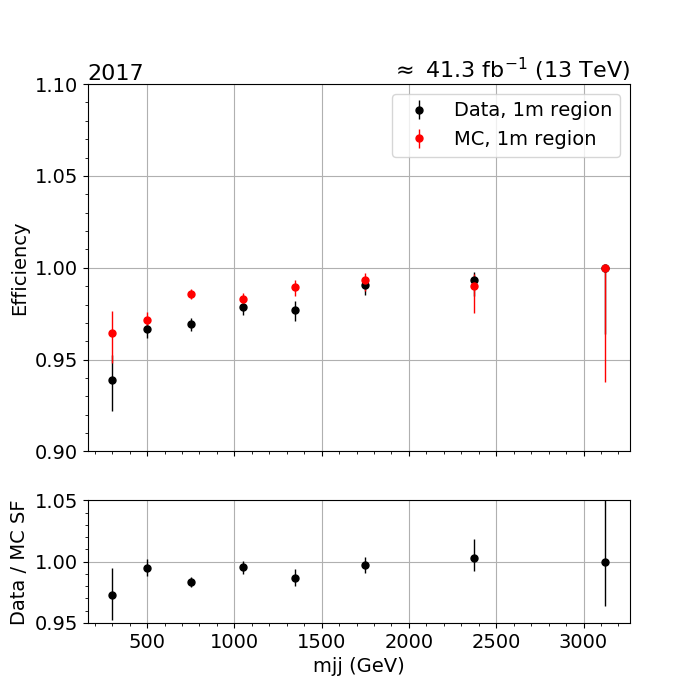
\includegraphics[width=0.49\textwidth]{fig/efficiency/trigger/met/mjj/data_mc_comparison_1m_2017_one_jet_forward_one_jet_central.png}
        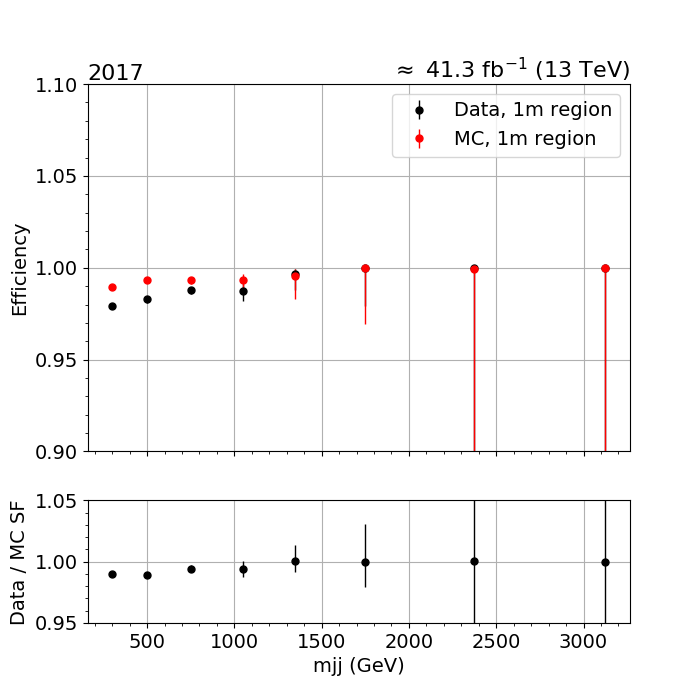
\includegraphics[width=0.49\textwidth]{fig/efficiency/trigger/met/mjj/data_mc_comparison_1m_2017_two_central_jets.png} \\
        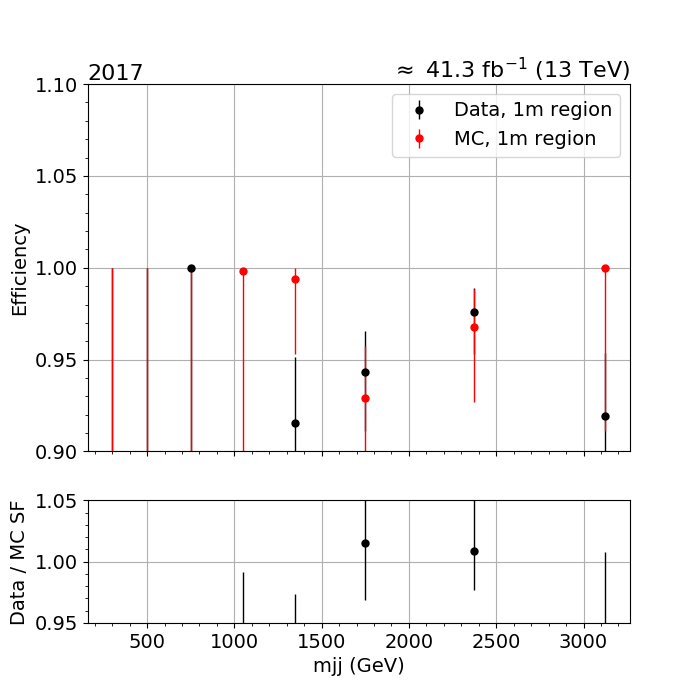
\includegraphics[width=0.49\textwidth]{fig/efficiency/trigger/met/mjj/data_mc_comparison_1m_2017_two_forward_jets.png}
    \end{center}
    \caption{MET trigger efficiency as a function of mjj in three categories: One forward jet and one central jet, two central jets and
            two forward jets. These results are obtained from 2017 data and MC samples with the selection of single muon events.} 
    \label{fig:eff_mjj_2017_1m}      
\end{figure}

\begin{figure}[hbp]
    \begin{center}
        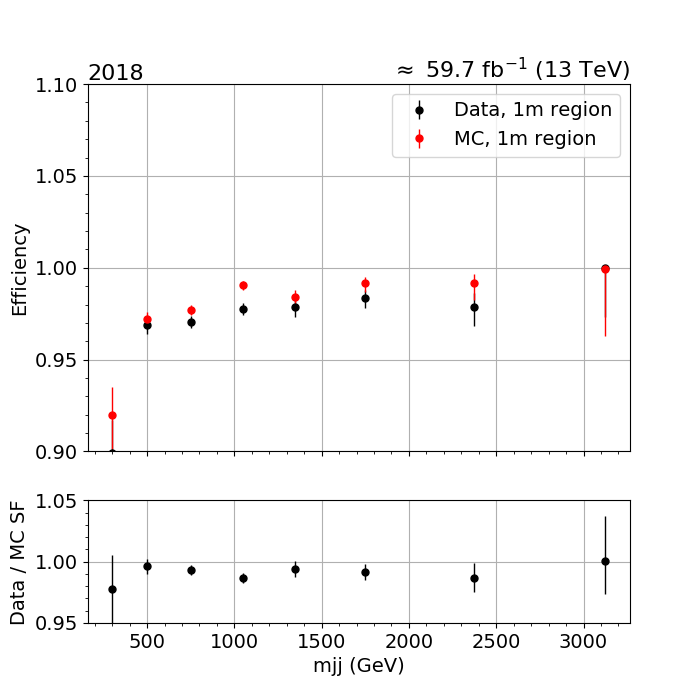
\includegraphics[width=0.49\textwidth]{fig/efficiency/trigger/met/mjj/data_mc_comparison_1m_2018_one_jet_forward_one_jet_central.png}
        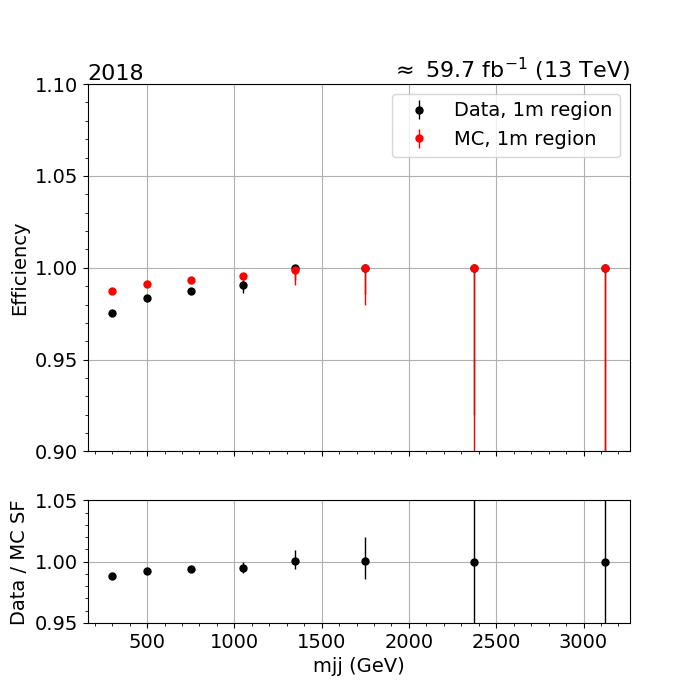
\includegraphics[width=0.49\textwidth]{fig/efficiency/trigger/met/mjj/data_mc_comparison_1m_2018_two_central_jets.png} \\
        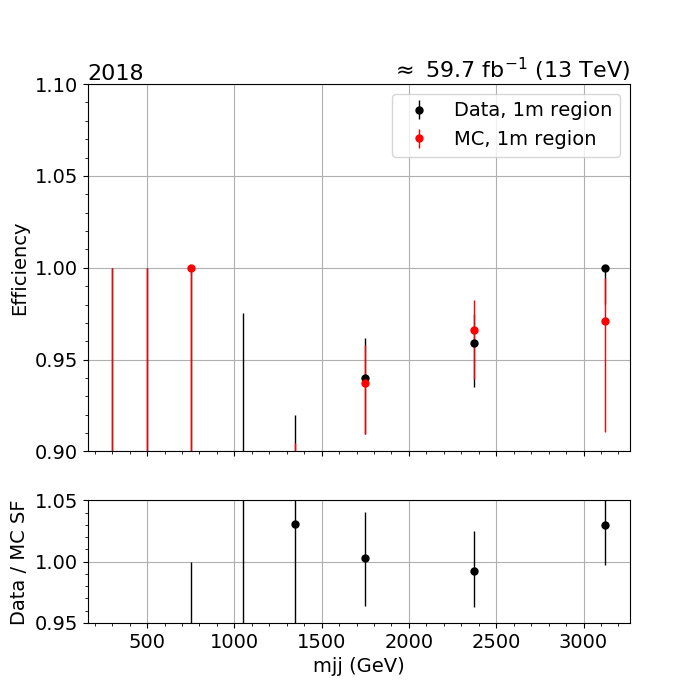
\includegraphics[width=0.49\textwidth]{fig/efficiency/trigger/met/mjj/data_mc_comparison_1m_2018_two_forward_jets.png}
    \end{center}
    \caption{MET trigger efficiency as a function of mjj in three categories: One forward jet and one central jet, two central jets and
            two forward jets. These results are obtained from 2018 data and MC samples with the selection of single muon events.}   
    \label{fig:eff_mjj_2018_1m}
\end{figure}

\begin{figure}[htp]
    \begin{center}
        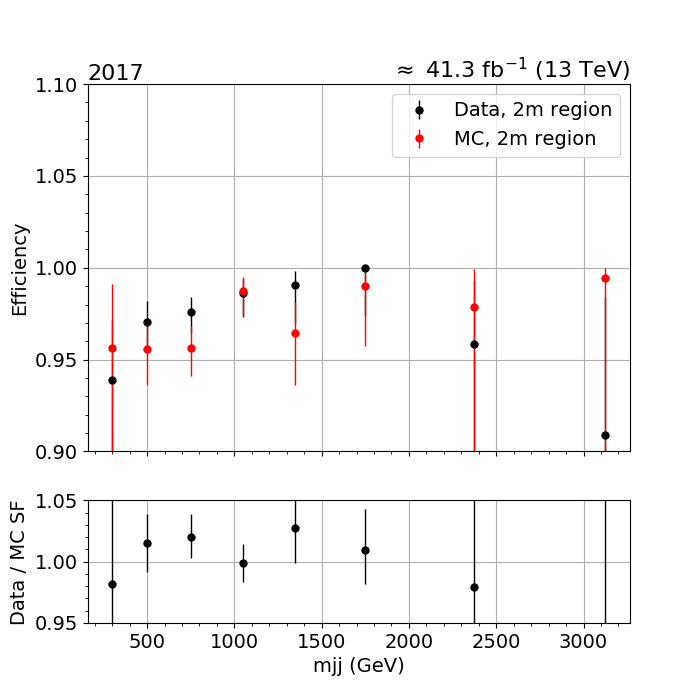
\includegraphics[width=0.49\textwidth]{fig/efficiency/trigger/met/mjj/data_mc_comparison_2m_2017_one_jet_forward_one_jet_central.png}
        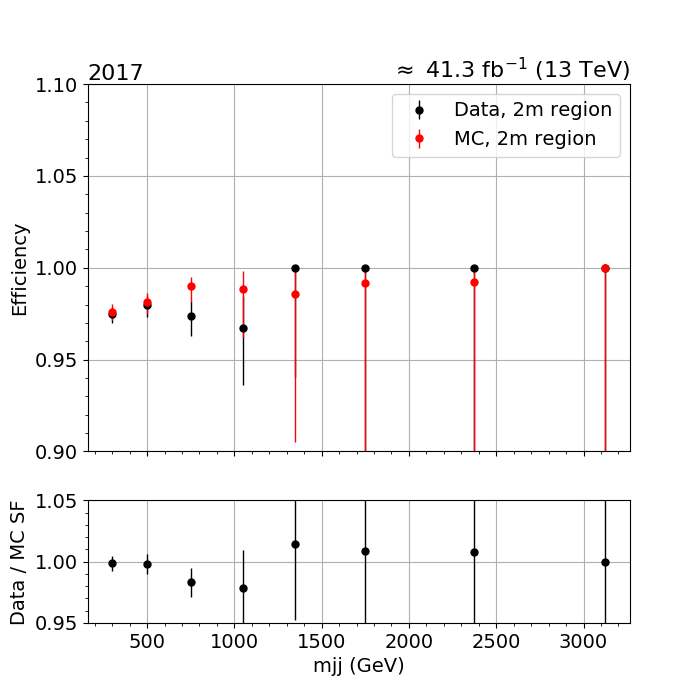
\includegraphics[width=0.49\textwidth]{fig/efficiency/trigger/met/mjj/data_mc_comparison_2m_2017_two_central_jets.png} \\
        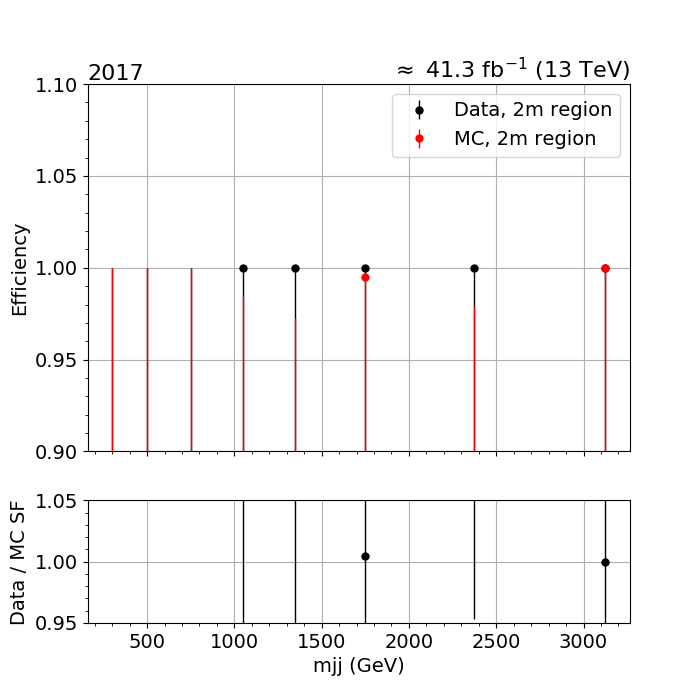
\includegraphics[width=0.49\textwidth]{fig/efficiency/trigger/met/mjj/data_mc_comparison_2m_2017_two_forward_jets.png}
    \end{center}
    \caption{MET trigger efficiency as a function of mjj in three categories: One forward jet and one central jet, two central jets and
            two forward jets. These results are obtained from 2017 data and MC samples with the selection of double muon events.}
    \label{fig:eff_mjj_2017_2m}
\end{figure}

\begin{figure}[hbp]
    \begin{center}
        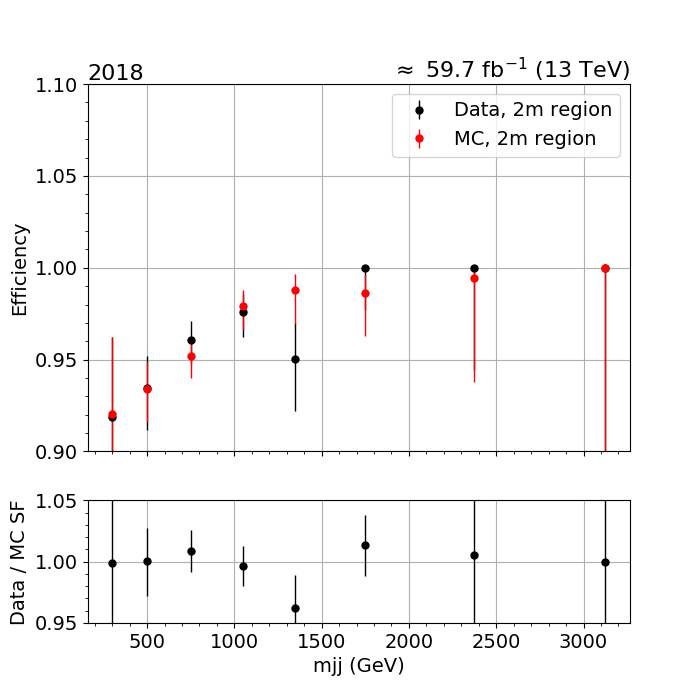
\includegraphics[width=0.49\textwidth]{fig/efficiency/trigger/met/mjj/data_mc_comparison_2m_2018_one_jet_forward_one_jet_central.png}
        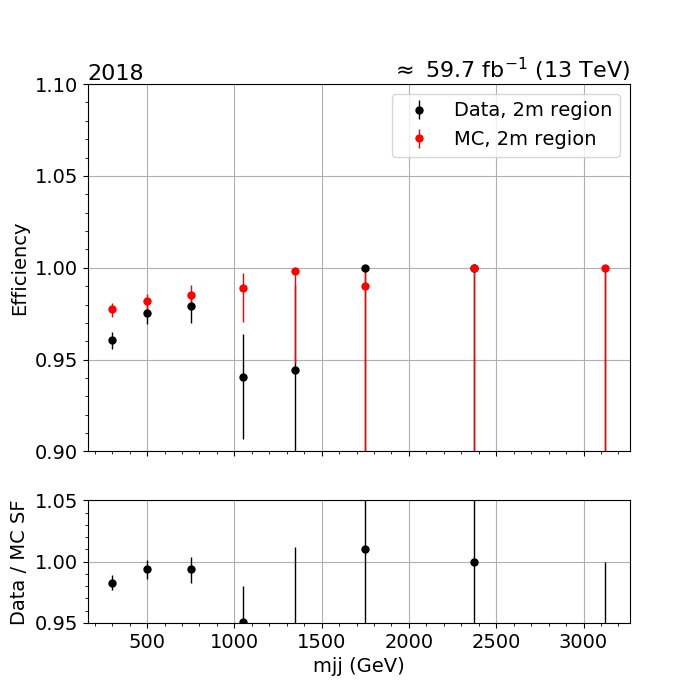
\includegraphics[width=0.49\textwidth]{fig/efficiency/trigger/met/mjj/data_mc_comparison_2m_2018_two_central_jets.png} \\
        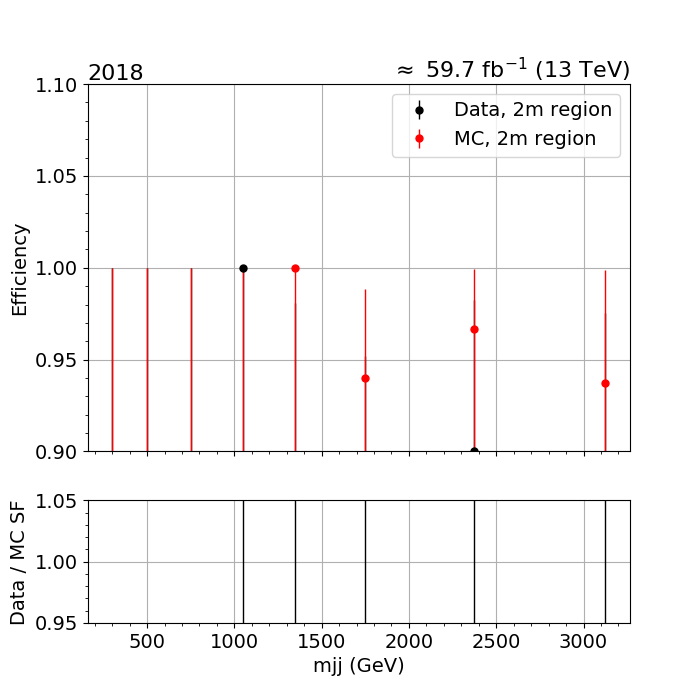
\includegraphics[width=0.49\textwidth]{fig/efficiency/trigger/met/mjj/data_mc_comparison_2m_2018_two_forward_jets.png}
    \end{center}
    \caption{MET trigger efficiency as a function of mjj in three categories: One forward jet and one central jet, two central jets and
            two forward jets. These results are obtained from 2018 data and MC samples with the selection of double muon events.}  
    \label{fig:eff_mjj_2018_2m}
\end{figure}

\begin{figure}[htp]
    \begin{center}
        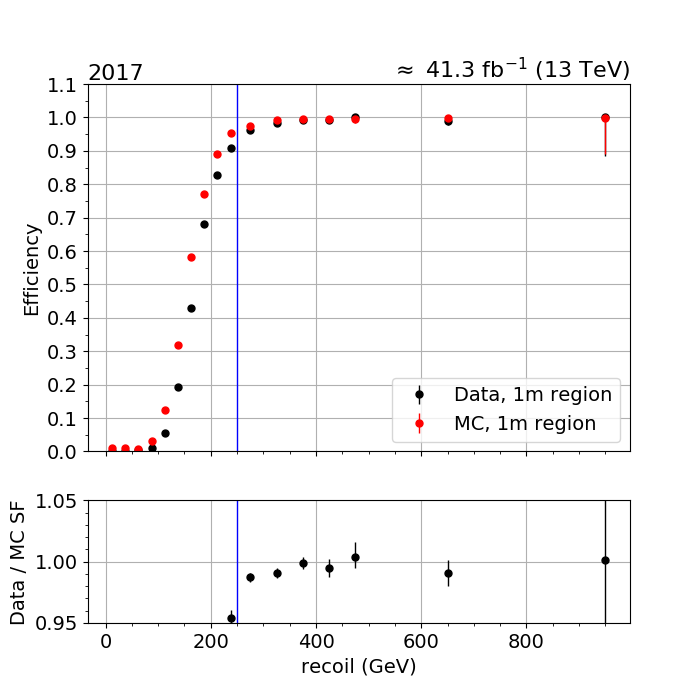
\includegraphics[width=0.49\textwidth]{fig/efficiency/trigger/met/recoil/data_mc_comparison_1m_2017_one_jet_forward_one_jet_central.png}
        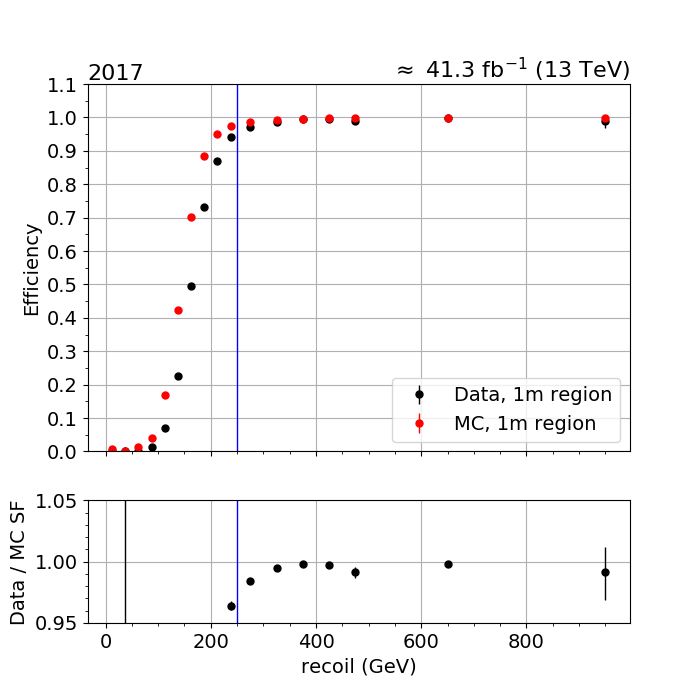
\includegraphics[width=0.49\textwidth]{fig/efficiency/trigger/met/recoil/data_mc_comparison_1m_2017_two_central_jets.png} \\
        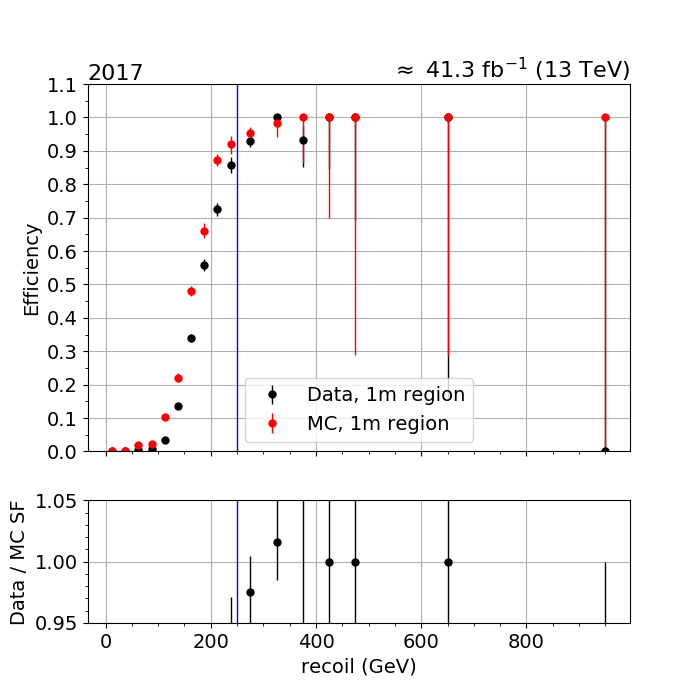
\includegraphics[width=0.49\textwidth]{fig/efficiency/trigger/met/recoil/data_mc_comparison_1m_2017_two_forward_jets.png}
    \end{center}
    \caption{MET trigger efficiency as a function of recoil in three categories: One forward jet and one central jet, two central jets and
            two forward jets. These results are obtained from 2017 data and MC samples with the selection of single muon events.} 
    \label{fig:eff_recoil_2017_1m}
\end{figure}

\begin{figure}[hbp]
    \begin{center}
        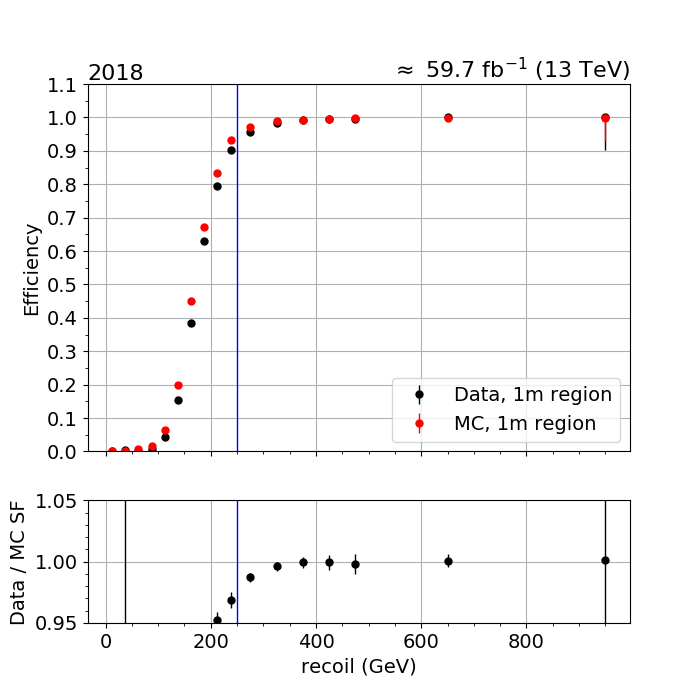
\includegraphics[width=0.49\textwidth]{fig/efficiency/trigger/met/recoil/data_mc_comparison_1m_2018_one_jet_forward_one_jet_central.png}
        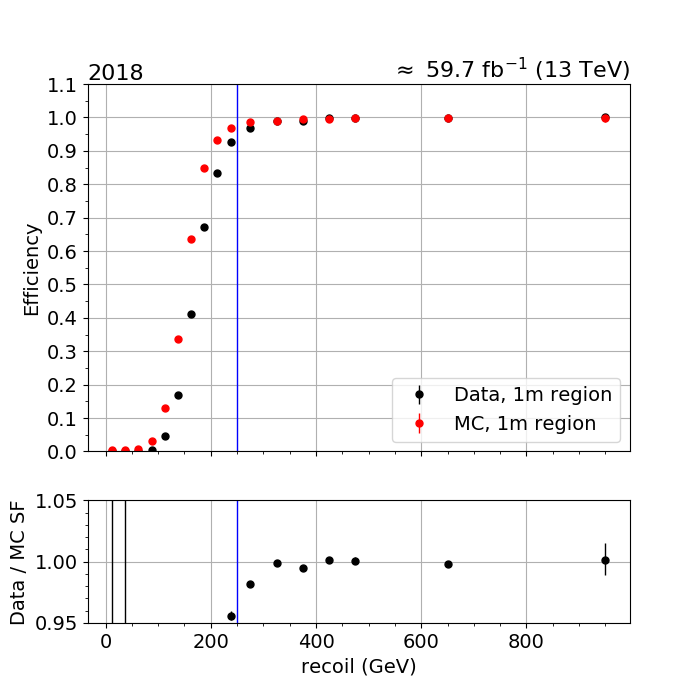
\includegraphics[width=0.49\textwidth]{fig/efficiency/trigger/met/recoil/data_mc_comparison_1m_2018_two_central_jets.png} \\
        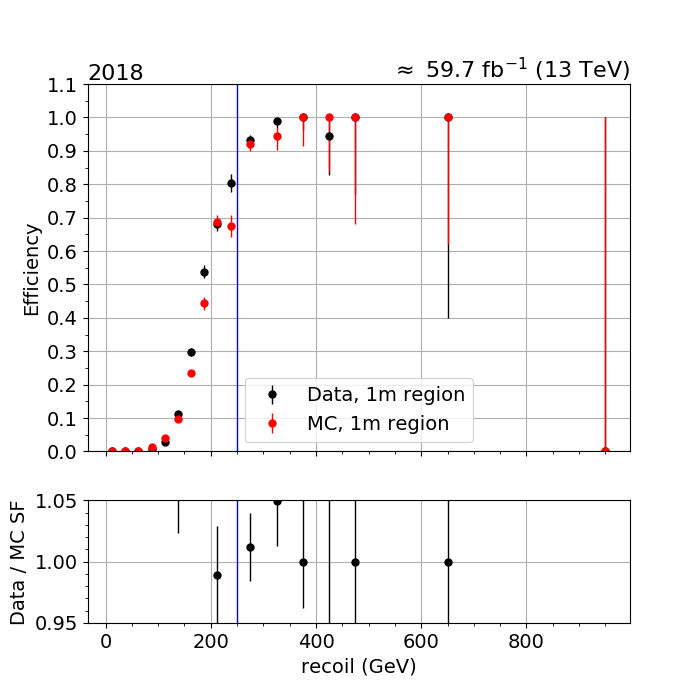
\includegraphics[width=0.49\textwidth]{fig/efficiency/trigger/met/recoil/data_mc_comparison_1m_2018_two_forward_jets.png}
    \end{center}
    \caption{MET trigger efficiency as a function of recoil in three categories: One forward jet and one central jet, two central jets and
            two forward jets. These results are obtained from 2018 data and MC samples with the selection of single muon events.}
    \label{fig:eff_recoil_2018_1m}
\end{figure}

\begin{figure}[htp]
    \begin{center}
        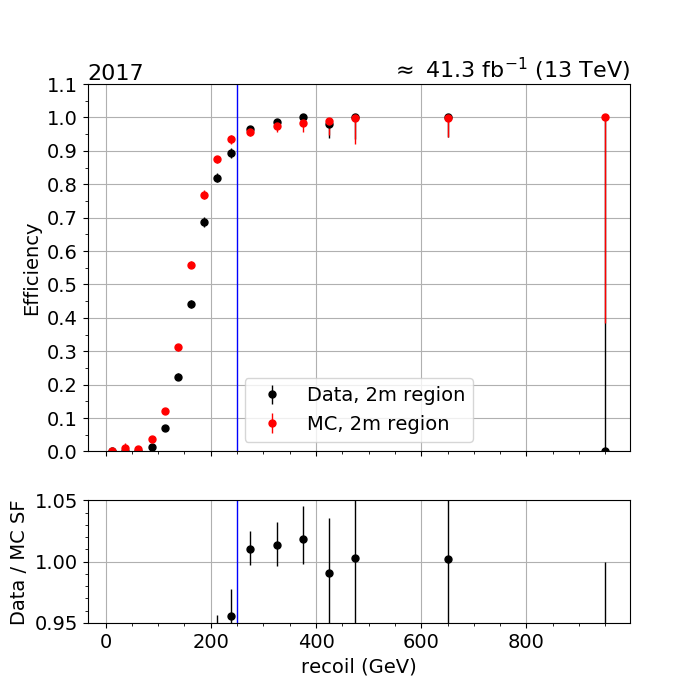
\includegraphics[width=0.49\textwidth]{fig/efficiency/trigger/met/recoil/data_mc_comparison_2m_2017_one_jet_forward_one_jet_central.png}
        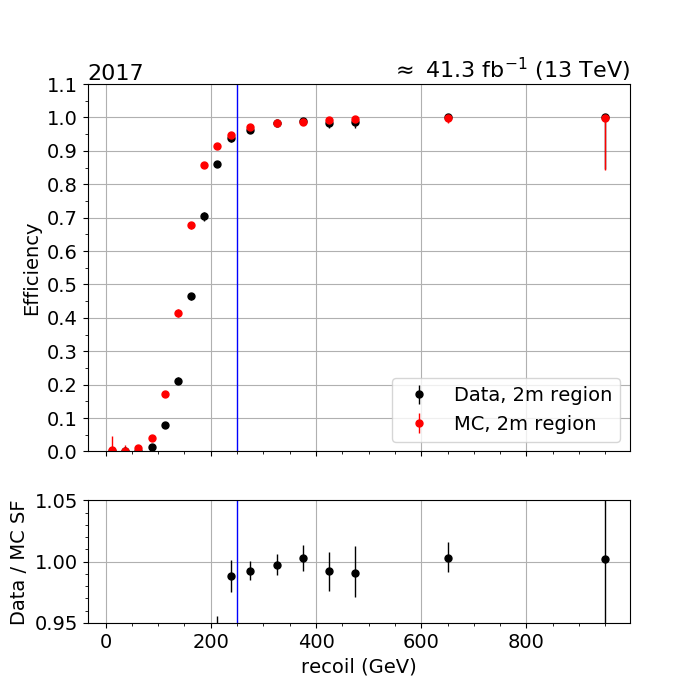
\includegraphics[width=0.49\textwidth]{fig/efficiency/trigger/met/recoil/data_mc_comparison_2m_2017_two_central_jets.png} \\
        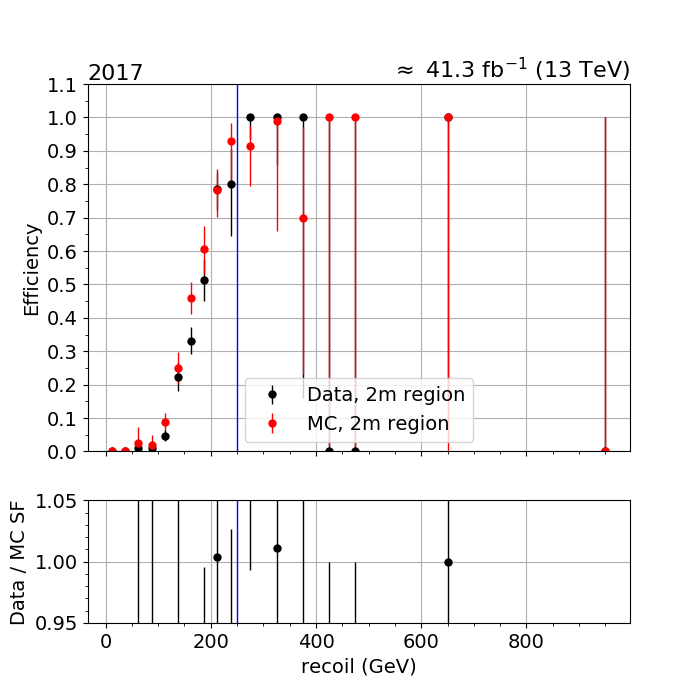
\includegraphics[width=0.49\textwidth]{fig/efficiency/trigger/met/recoil/data_mc_comparison_2m_2017_two_forward_jets.png}
    \end{center}
    \caption{MET trigger efficiency as a function of recoil in three categories: One forward jet and one central jet, two central jets and
            two forward jets. These results are obtained from 2017 data and MC samples with the selection of double muon events.}   
    \label{fig:eff_recoil_2017_2m}
\end{figure}

\begin{figure}[hbp]
    \begin{center}
        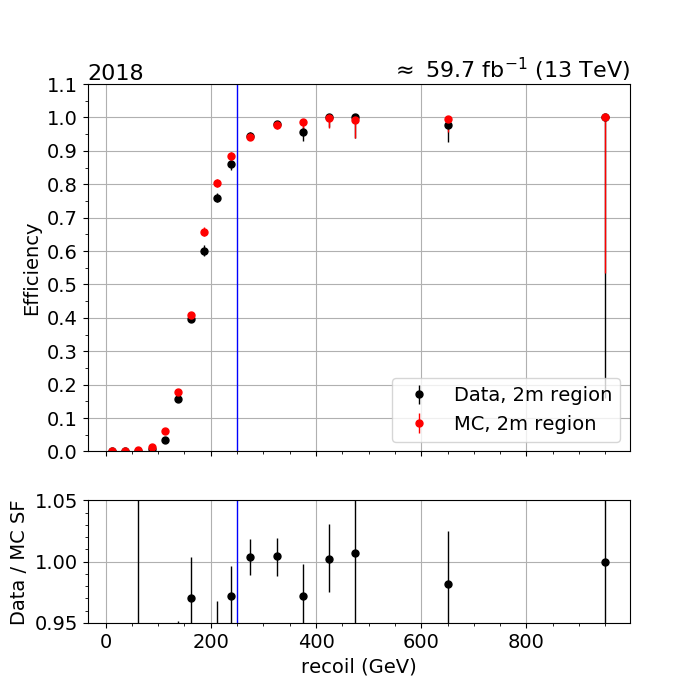
\includegraphics[width=0.49\textwidth]{fig/efficiency/trigger/met/recoil/data_mc_comparison_2m_2018_one_jet_forward_one_jet_central.png}
        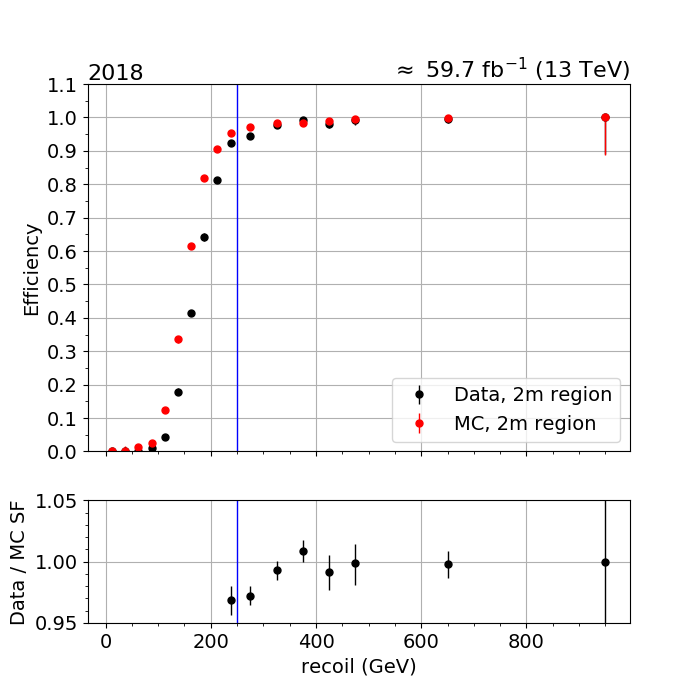
\includegraphics[width=0.49\textwidth]{fig/efficiency/trigger/met/recoil/data_mc_comparison_2m_2018_two_central_jets.png} \\
        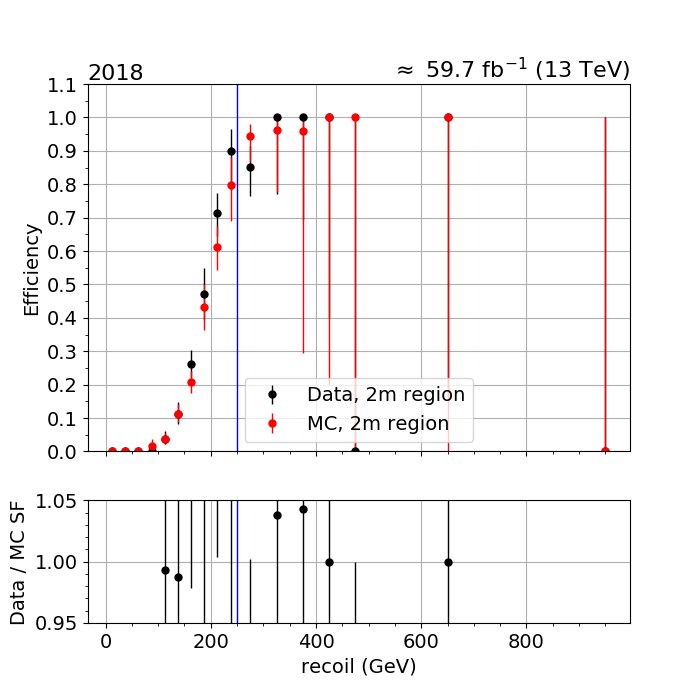
\includegraphics[width=0.49\textwidth]{fig/efficiency/trigger/met/recoil/data_mc_comparison_2m_2018_two_forward_jets.png}
    \end{center}
    \caption{MET trigger efficiency as a function of recoil in three categories: One forward jet and one central jet, two central jets and
            two forward jets. These results are obtained from 2018 data and MC samples with the selection of double muon events.}  
    \label{fig:eff_recoil_2018_2m}
\end{figure}
\section{Physics objects} \label{sec:objects}

All physics objects are used to identify signal-like events, to suppress backgrounds and to define control regions
for background estimation. For the object definitions, we mostly follow the CMS POG endorsed recommendations. The physics 
objects and the selection requirements are described below.

\subsection{Jets}
\label{sec:objects_ak4}
In this analysis, jets are reconstructed by clustering PF candidates
using the infrared and collinear safe anti-\kt algorithm~\cite{Cacciari:2008gp}. Jets are clustered
with a distance parameter of 0.4 and are referred to as AK4 jets.
The reconstructed vertex with the largest value of summed physics-object $\pt^2$ is taken to
be the primary $\Pp\Pp$ interaction vertex. The physics objects are those returned by a
jet finding algorithm~\cite{Cacciari:2008gp,Cacciari:2011ma} applied to all charged PF candidates
associated with the vertex, plus the corresponding associated missing transverse momentum.

Jet momentum is determined as the vector sum of all particle momenta in the jet,
and is found from simulation to be within 5 to 10\% of the true momentum over the full \pt
spectrum and detector acceptance. An offset correction is applied to jet energies to take
into account the contribution from additional proton-proton interactions within the
same or nearby bunch crossings (pileup). Jet energy corrections are derived from simulation,
and are confirmed with {\it in situ} measurements of the energy balance in dijet, multijet,
$\gamma$+jet, and leptonic Z+jet events~\cite{Khachatryan:2016kdb}. The \texttt{Fall17\_17Nov2017\_V32} and \texttt{Autumn18\_V8}
versions of the jet energy corrections are used for the 2017 and 2018 data sets, respectively.

The AK4 jets used in this analysis are required to pass loose jet identification criteria.
In addition, all the jets with \pt smaller than $50 GeV$ must pass the medium pileup ID criteria. This additional constraint
on all AK4 jets is found to improve the modeling of jet distributions, especially in the horn regions near $|\eta| = 2.9$. 
The effect of this requirement is demonstrated in the sub-leading jet $\eta$ distribution in Fig.~\ref{fig:pileupid}.

\begin{figure}[htbp]
  \centering
        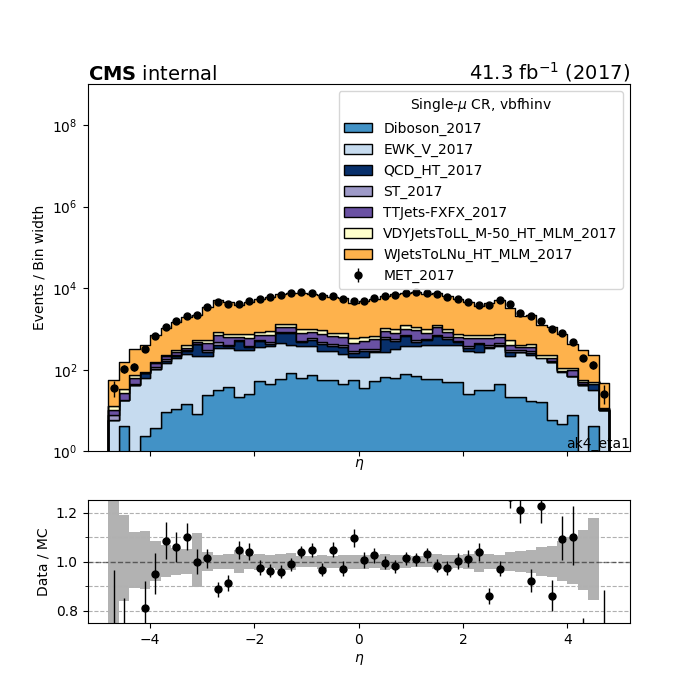
\includegraphics[width=0.45\textwidth]{fig/datamc/cr_1m_vbf/cr_1m_vbf_ak4_eta1_losf_2017_withpuid.png}
        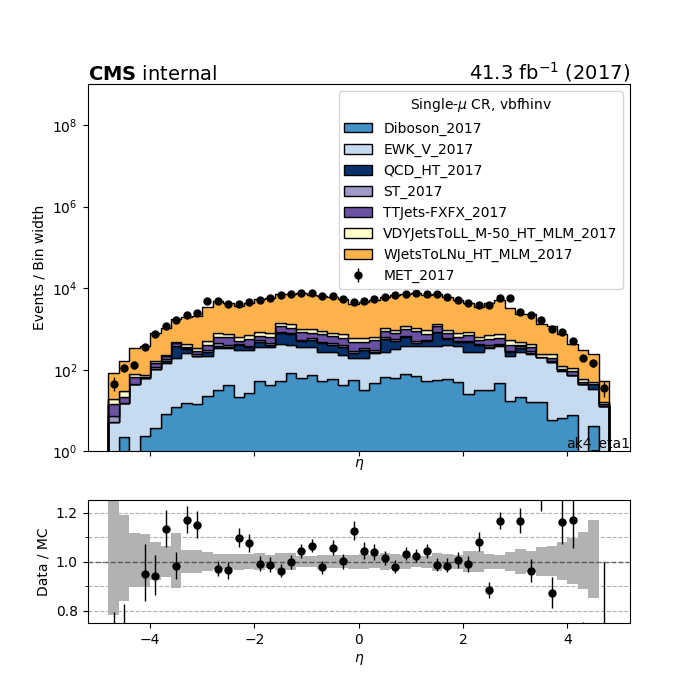
\includegraphics[width=0.45\textwidth]{fig/datamc/cr_1m_vbf/cr_1m_vbf_ak4_eta1_losf_2017_withoutpuid.png}
  \caption{Subleading AK4 jet $\eta$ distribution with pileup ID requirement (left) and without pileup ID requirement (right) in the single muon control region.}
  \label{fig:pileupid}
\end{figure}

{\color{red} Need to add information about JER correction usage}

Lastly, to suppress the contributions due to non-collision backgrounds, the following
requirements are applied on the leading AK4 jet:
\begin{itemize}
\item Charged hadron energy fraction $> 0.1$
\item Neutral hadron energy fraction $< 0.8$
\end{itemize}

\subsubsection{b-tagged jets}

%{\color{red} Update the b-tagging working point when the new tagging working points are defined}
In this analysis b jets with $\pt > 20$~\GeV and $|\eta| < 2.4$ are identified
using the ``DeepCSV'' algorithm~\cite{Sirunyan:2017ezt},
adopting a working point (medium) corresponding to correctly identifying a b-jet with a
probability of 80\%, and misidentifying a light-flavor jet with a probability of 10\%.
This working point corresponds to the value of DeepCSV tagger to be greater than 0.4941.
Events with identified b jets are rejected to reduce the contamination from top quark processes.

\subsection{Missing transverse momentum and recoil}

The vector \ptvecmiss is defined as the imbalance in the transverse
momentum of all particles that interact with the detectors.
Due to momentum conservation in the plane transverse to the beam axis, \ptvecmiss
corresponds to the transverse momentum that is carried by undetected particles such as neutrinos.
Practically, \ptvecmiss is computed as the negative of the vectorial sum of transverse
momenta of all PF candidates and is therefore also referred to as PF \ptvecmiss. 
The magnitude of the \ptvecmiss is referred to as \ptmiss.

Minimum energy thresholds in the calorimeters, inefficiencies
in the tracker, nonlinearity of the response of the calorimeter
for hadronic particles can lead to an over- or underestimation of \ptmiss.
The bias on the \ptmiss measurement is reduced by propagating the effect of the jet energy
corrections introduced in section~\ref{sec:objects_ak4} according to

\begin{equation}
\ptvecmiss(\mathrm{corr})
=\ptvecmiss - \sum_\mathrm{jets} (\vec{p}_\mathrm{T,jet}({\mathrm{corr}})-\vec{p}_\mathrm{T,jet}),
\label{eq:Type1MET}
\end{equation}
where the ``corr'' refers to the scale energy corrected measurements
of the related objects.

This ``type-I'' correction for \ptvecmiss uses jet energy scale corrections
for all corrected jets with $\pt>15\GeV$ that have less than $0.9$
of their energy deposited in the ECAL. Furthermore, if a muon is found in a
jet, its 4-momentum is subtracted from the 4-momentum of the jet
when performing the correction and is added back to a corrected object.

Since signal events in this analysis contain only jets and no other reconstructed candidates,
\ptmiss is equivalent to the total hadronic momentum in the event. For the leading backgrounds, 
this also corresponds to the transverse momentum of the W or Z boson. 
To mimic this behavior in in the control regions of this analysis, the transverse
momentum of the hadronic recoil $\vec{U}$, defined as the vectorial sum of the transverse
momenta of all particles except the vector boson (or its decay products), is used.
The variable is  computed as
\begin{equation}
  \vec{U} = \ptvecmiss + \sum _{i\;\in\;\textrm{leptons, photons}}\vec{p}^{i}_{T}}
\end{equation}

where the sum takes into account the leptons and photons used to define the respective control region.
The uncertainty of \ptmiss has a strong dependence on the
event topology. Therefore, the uncertainty on \ptmiss is often factorized into its components of
jets, leptons and unclustered energy. Each sub-component is then varied
within its scale and resolution uncertainty. In this analysis, the largest
contribution on the final \ptmiss uncertainty comes from the variations of the
jet energy scale correction and the magnitude of the uncertainty is estimated
to be 4\% for the \Zvvjets~events. This uncertainty is not the most recent one and it will be recalculated.

Anomalous high-\ptmiss events can appear due to various phenomena.
In the ECAL, spurious deposits may appear due to particles striking
sensors in the ECAL photodetectors, or from real showers with non-collision
origins such as those caused by beam halo particles. ECAL dead cells can cause real
energy to be missed, again leading to a spurious imbalance.
In the HCAL, spurious energy can arise due to  noise in the hybrid
photodiode and readout box  electronics, as well as
direct particle interactions with  the light guides and
photomultiplier tubes of the forward calorimeter. 
A number of filters has been developed by the POG/DPG groups to identify and supress anomalous high
\ptmiss events~\cite{CMS-JME-TWIKI-FILTER}. The recommended filters are listed in Tab.~\ref{tab:metfilters} and are applied in the analysis.

\begin{table}[ht!]
    \centering
    \small
    \def\arraystretch{1.5}
    \caption{The \ptmiss filters recommended by the JME POG~\cite{CMS-JME-TWIKI-FILTER}. The recommendations apply to both 2017 and 2018. Except for the bad super cluster filter (``ee badSC''), all filters are applied both in data and simulation.}
    \begin{tabular}{l l c }
        \hline
        \hline
                                           &                                                                     \\
        Filter                             & Name in NanoAOD                          & Applied in data (MC)     \\\hline
        primary vertex filter              & Flag\_goodVertices                       & \checkmark  (\checkmark) \\
        beam halo filter                   & Flag\_globalSuperTightHalo2016Filter     & \checkmark  (\checkmark) \\
        HBHE noise filter                  & Flag\_HBHENoiseFilter                    & \checkmark  (\checkmark) \\
        HBHEiso noise filter               & Flag\_HBHENoiseIsoFilter                 & \checkmark  (\checkmark) \\
        ECAL TP filter                     & Flag\_EcalDeadCellTriggerPrimitiveFilter & \checkmark  (\checkmark) \\
        Bad PF Muon Filter                 & Flag\_BadPFMuonFilter                    & \checkmark  (\checkmark) \\
        ee badSC noise filter              & Flag\_eeBadScFilter                      & \checkmark  (\times)     \\
        ECAL bad calibration filter update & Flag\_ecalBadCalibFilterV2               & \checkmark  (\checkmark) \\
        \hline
    \end{tabular}

    \label{tab:metfilters}
\end{table}

To further miminize the contribution of anomalous high-\ptmiss events
(specifically due to spurious charged hadrons) in this analysis, a
quantity based on the relative ratio of calorimetry based \ptmiss and
PF based \ptmiss is employed. Events satisfying $|\metcalo - \metpf|/U < 0.5$ 
are selected in this analysis.

\subsection{Leptons}

\subsubsection{Electrons}

Electrons within the geometrical acceptance of $|\eta| < 2.5$
are reconstructed by associating tracks reconstructed
in the silicon detector with clusters of energy in the ECAL~\cite{Khachatryan:2015hwa}.
Well-identified electron candidates are required to satisfy
additional identification criteria based on the shower
shape of the energy deposit in the ECAL and the consistency of the
electron track with the primary vertex~\cite{TRK-11-001}. Electron candidates
that are identified as coming from photon conversions in
the detector material are removed. An isolation variable is calculated based on the sum of the energies of the PF candidates 
within a cone of $\Delta R < 0.3$ around the electron. The mean energy deposit in the isolation cone of the electron coming 
from pileup is estimated following the method described in Ref.~\cite{Khachatryan:2015hwa} and subtracted from the isolation sum. 
In this note, `veto'~\cite{CMS-EGM-TWIKI-ELEID} electrons with a minimum $\pt$ of 10~\GeV are selected with an average efficiency 
of 95\% and their presence is used as a condition to reject events, whereas `tight'~\cite{CMS-EGM-TWIKI-ELEID} electrons with a 
minimum $\pt$ of 40~\GeV and an average efficiency of 70\% are used to select the events
in the control regions. Full selection criteria are shown in Table~\ref{tab:ElectronIDTight}.

\begin{table}[htb]
    \centering
    \small
    \def\arraystretch{1.5}
    \caption{Tight and veto electron identification criteria.}

    \begin{tabular}{ l c c}
        \hline\hline
        Variable                                                & Selection Tight                              & Selection Veto                             \\
                                                                & Barrel (Endcaps)                             & Barrel (Endcap)                            \\
        \hline
        \hline
        \multirow{2}{*}{Full 5x5 $\sigma_{i\eta i\eta}$}        & $< 0.0104  $                                 & $< 0.0126   $                              \\
                                                                & ($< 0.0353   $)                              & ($< 0.0457   $)                            \\\cline{2-3}
        \multirow{2}{*}{$|\Delta \eta_{in}|$}                   & $< 0.00255  $                                & $< 0.00463  $                              \\
                                                                & ($< 0.00501  $)                              & ($< 0.00814   $)                           \\\cline{2-3}
        \multirow{2}{*}{$|\Delta \phi_{in}|$}                   & $< 0.022   $                                 & $< 0.148    $                              \\
                                                                & ($< 0.0236   $)                              & ($< 0.19    $)                             \\\cline{2-3}
        \multirow{2}{*}{H/E}                                    & $< 0.026+1.15/E_{SC}+0.0324\rho/E_{SC}  $    & $< 0.05+1.16/E_{SC}+0.0324\rho/E_{SC}   $  \\
                                                                & ($< 0.0188+2.06/E_{SC}+0.183*\rho/E_{SC}  $) & ($< 0.05+2.54/E_{SC}+0.183\rho/E_{SC}   $) \\\cline{2-3}
        \multirow{2}{*}{Relative isolation ($\rho$ correction)} & $< 0.0287+0.506/pT  $                        & $< 0.198+0.506/\pt   $                     \\
                                                                & ($< 0.0445+0.963/\pt  $)                     & ($< 0.203+0.963/\pt   $)                   \\\cline{2-3}
        \multirow{2}{*}{1/E - 1/p}                              & $< 0.159   $                                 & $< 0.209    $                              \\
                                                                & ($< 0.0197   $)                              & ($< 0.132    $)                            \\\cline{2-3}
        \multirow{2}{*}{$|\mathrm{d_{xy}(vtx)}|$}               & $< 0.050   $                                 & $< 0.050 $                                 \\
                                                                & ($< 0.100   $)                               & ($< 0.100   $)                             \\\cline{2-3}
        \multirow{2}{*}{$|\mathrm{d_{z}(vtx)}|$}                & $< 0.100   $              & $< 0.100 $            \\
                                                                & ($< 0.200   $)                               & ($< 0.200   $)                             \\\cline{2-3}
        \multirow{2}{*}{Expected Inner Missing Hits}            & $<= 1$                                       & $<= 2 $                                    \\
                                                                & ($<= 1$)                                     & ($<= 3$)                                   \\\cline{2-3}
        \multirow{2}{*}{Pass conversion veto}                   & Yes                                          & Yes                                        \\
                                                                & (Yes)                                        & (Yes)                                      \\
        \hline\hline
    \end{tabular}
    \label{tab:ElectronIDTight}
\end{table}



\subsubsection{Muons}

Muons within the geometrical acceptance of $|\eta| < 2.4$ are reconstructed by combining information from the silicon tracker 
and the muon system~\cite{Chatrchyan:2012xi}. The muons are required to pass set of quality criteria based on the number of spatial 
points measured in the tracker and in the muon system, the fit quality of the muon track and its consistency with the primary vertex 
of the event. Similar to electron case, the isolation requirements for muons are also based on the sum of the energies of the PF candidates, 
but a different cone size of a $\Delta R < 0.4$ is used. The muon isolation variable is corrected for pileup effects by subtracting half 
of the sum of the transverse momenta of charged particles that are inside the isolation cone and not associated with the primary vertex. 
In this note, ``loose''~\cite{CMS-MUO-TWIKI-IDLOOSE} muons with $\pt>10~\GeV$ are selected with an average efficiency of 98\% and 
are used as a condition to reject events,whereas ``tight''~\cite{CMS-MUO-TWIKI-IDTIGHT} muons with $\pt>20~\GeV$ are selected with an 
average efficiency of 95\% and are used to select events in the control samples. 
A full list of tight identification criteria is given here:

\begin{itemize}
\item Muon reconstructed as a global muon
\item Muon reconstructed as a particle flow muon
\item Normalized $\chi^2$ of the global track less than 10
\item At least one muon chamber hit included in the global track fit
\item Muon segments in at least two muon stations
\item Transverse impact parameter w.r.t. the primary vertex less than $2$ mm.
\item Longitudinal impact parameter w.r.t. the primary vertex less than $5$ mm.
\item At least one pixel hit
\item Hits on at least 5 tracker layers
\item $\Delta\beta$ relative isolation less than 0.15
\end{itemize}

\subsubsection{Taus}

Hadronically decaying $\tau$ leptons are required to pass identification criteria
using the hadron-plus-strips algorithm~\cite{Khachatryan:2015dfa}. The algorithm
identifies a jet as an hadronically decaying tau lepton candidate if a subset of the
particles assigned to the jet is consistent with the decay products of a $\tau$ candidate.
Candidate $\tau$ jets are reuired to pass both the ``DecayModeNewDMs'' and ``DecayMode'' identifiers.

In addition, $\tau$ candidates are required to be isolated from other activity in the
event. The isolation requirement is computed by summing the \pt of the charged PF
candidates and PF photon candidates within an isolation cone of $\Delta R = 0.5 (0.3)$,
around the tau candidate direction. The charged and photon candidates associated with the
tau candidate are removed from this sum and further described in Ref.~\cite{Khachatryan:2015dfa}.
The ``VLoose\_IsolationMVArun2v1DBnewDMwLT'' isolation working point~\cite{taupog_twiki} is employed in this analysis
for tau candidates with \pt larger than 18~\GeV within $|\eta| < 2.3$.


\subsection{Photons}

Photon candidates are reconstructed from energy deposits in the ECAL using algorithms
that constrain the clusters to the size and shape expected from a photon~\cite{CMS:EGM-14-001}.
The identification of the candidates is based on shower-shape and isolation variables.
For isolated photons, scalar sums of the \pt of PF candidates within a cone of $\Delta R < 0.3$
around the photon candidate are required to be below the bounds defined. Only the PF candidates
that do not overlap with the EM shower of the candidate photon are included in the isolation sums.
The photon candidates used in this analysis are required to have a minimum transverse momentum of 15~\GeV and to
be within $|\eta| < 2.5$ passing the `loose'~\cite{CMS-EGM-TWIKI-GAMID} identification criteria in.
The full identification criteria is also given in Table~\ref{tab:PhotonIDLoose}.

\begin{table}[htb!]
\centering
\small
\def\arraystretch{1.2}
\begin{tabular}{l c}
\hline
Variable                                   &  Selection       \\
                                           &  Barrel (Endcap)  \\
\hline
\hline
Full 5x5 $\sigma_{i\eta i\eta}$            & $< 0.0106 $ ($< 0.0272 $)    \\
H/E                                        & $<  0.04596 $ ($< 0.0590 $)    \\
charged hadron isolation                   & $< 1.694 $  ($< 2.089 $)     \\
neutral hadron isolation                   & $< 24.032 (19.722) + 0.01512(0.0117)\times p_T+2.259(2.3)\times 10^{-5} \times {p_T}^2$ \\
photon isolation                           & $< 2.876 (4.162) + 0.004017(0.0037)\times p_T$  \\
Conversion safe electron veto              & Yes (Yes)           \\
\hline
\end{tabular}
\caption{Loose photon identification criteria.}
\label{tab:PhotonIDLoose}
\end{table}

\subsubsection{Photon purity studies}
{\color{red} To be added.}
\section{Reweighting of simulated events} \label{sec:reweighting}

Simulated signal and background samples are corrected for various effects through reweighting procedures outlined in this section.

\subsection{Trigger efficiency reweighting}

\subsubsection{\ptmiss+\mht triggers}
The performance of the \ptmiss+\mht triggers is measured using single muon events. The
events are selected from the SingleMuon using the \texttt{HLT\_IsoMu27} (\texttt{HLT\_IsoMu24}) trigger for 2017 (2018), and the offline muon is required to be well-identified and have \pt larger than 40 GeV. The same selection is required as for the single-muon control region used in the final fit (cf. sec. ~\ref{sec:selection_cr_1m}):

\begin{enumerate}
\item Veto on additional leptons, photons, b jets, $\tau_{had}$ candidates.
\item $\Delta\phi(jet,\ptvecmiss)>0.5$ for the four leading jets with $\pt>30~\GeV$.
\item (Calo \ptmiss - PF \ptmiss) / recoil < 0.5
\item $M_{T}(\ell,\ptmiss) > 160~\GeV$.
\item Central AK4 jet with $\pt>100 GeV$, passing the tight jet ID.
\end{enumerate}

The efficiency is calculated as a function of the hadronic recoil \pt and is shown in Fig.~\ref{fig:hlteff_met}.
The trigger is found to be more than $95\%$ efficient for events with a recoil larger than $250~\GeV$, and more than $99\%$ efficient for events with a recoil larger than $375~\GeV$. The MC-to-data scale factor is found to be within $1\%$ of unity everywhere except for the lowest recoil bin at $250~\GeV$, where it is within $2\%$.

To investigate the stability of the measurement in single muon events, the same method is used to extract the efficiency from samples of double muon and single electron events. Again, an identical selection to the analysis control regions is used (cf. sec. ~\ref{sec:selection_cr_2m} and~\ref{sec:selection_cr_1e}), with the exception of requiring the leading muon \pt to be larger than 40~\GeV and omitting the \ptmiss cut in the electron region. The \HT-binned \texttt{WJets} and \texttt{DYJets} simulation samples are used. The resulting data-to-MC efficiency scale factors for all regions are shown in Fig.~\ref{fig:hltsf_met}. For 2017, a clear trend is present: The scale factor in dimuon events is larger in absolute terms then the one from the single muon region, and the scale factor from single electron events is the smallest. The difference between all regions is within $1\%$ relative to the single muon region. For 2018, -- clear trend is observed above a recoil of $250~\GeV$: The scale factors from all three regions agree within the available statistical precision. Finally, the scale factors obtained form the single muon region are used to reweight the simulation. The difference to the other regions is taken into account by assigning an overall $1\%$ uncertainty.

\begin{figure*}[hbtp]\begin{center}
    \includegraphics[width=0.49\textwidth]{fig/efficiency/trigger/met/data_mc_comparison_1m_2017.pdf}
    \includegraphics[width=0.49\textwidth]{fig/efficiency/trigger/met/data_mc_comparison_1m_2018.pdf}
    \caption{MET trigger turn-on curve measured in single muon events as a function of hadronic recoil \pt in the 2017 and 2018 \texttt{SingleMuon} datasets and \HT-binned \texttt{WJets} simulation samples. The vertical blue line indicates a recoil value of $250~\GeV$, which is the requirement used in the analysis selection. The bottom panel shows the MC-to-data scale factor, with the blue horizontal lines indicating deviations of $1\%$ and $2\%$ from unity, respectively.}
    \label{fig:hlteff_met}
 \end{center}\end{figure*}

\begin{figure*}[hbtp]\begin{center}
    \includegraphics[width=0.49\textwidth]{fig/efficiency/trigger/met/sf_comparison_2017.pdf}
    \includegraphics[width=0.49\textwidth]{fig/efficiency/trigger/met/sf_comparison_2018.pdf}
    \caption{MC-to-data efficiency scale factors measured single muon events (`1m'), dimuon events (`2m') and single electron events (`1e'). For the single-lepton regions, the \HT-binned \texttt{WJets} are used, and the \HT-binned \texttt{DY} samples are used for the dimuon region. The bottom panel shows the ratio of the scale factors obtained from each individual region to the scale factor obtained from the single muon region. The vertical blue line indicates a recoil value of $250~\GeV$, which is the requirement used in the analysis selection, while the horizontal lines indicate deviations of $\pm1\%$ from unity.}
    \label{fig:hltsf_met}
 \end{center}\end{figure*}



\subsubsection{Photon trigger}
The photon trigger efficiency is measured using events from the JetHT dataset collected with the \texttt{HLT\_PFHT1050} trigger, which was fully unprescaled in 2017 and 2018~\footnote{The other, prescaled \texttt{HLT\_PFHTXXX} paths yield lower statistical precision.}. Events are selected in the same way as for the photon analysis control region (cf. sec.~\ref{sec:selection_cr_g}), except for the photon \pt, recoil and trigger requirements. The trigger efficiency $\epsilon$ is then determined as:

$$\epsilon(\texttt{HLT\_Photon200}) = \frac{\text{Offline selection \&\& \texttt{HLT\_PFHT1050} \&\& \texttt{HLT\_Photon200}}}{\text{Offline selection \&\& \texttt{HLT\_PFHT1050}}} $$

The resulting efficiency in data and \texttt{GJets} \HT-binned simulation is shown in Fig.~\ref{fig:hlteff_photon}. The trigger efficiency in data is larger than $95\%$ for a photon \pt of larger than $215~\GeV$, and larger than $99\%$ for photon \pt larger than $400~\GeV$. Between $250$ and $400~\GeV$, there is a slight inefficiency amounting to approximately $1\%$ at the most, with a larger amplitude in 2017 than in 2018. In both years, the turn-on behavior is almost immediate in simulated events, resulting in an MC-to-data scale factor almost entirely driven by the efficiency in data. The scale factor is within $1\%$ of unity for all bins except the lowest 2017 bin at $215\~GeV$, where is deviates from unity by about $4\%$.

Based on these results, the offline \pt cut for the photon in the photon control region is chosen to be $215~\GeV$.

\begin{figure*}[hbtp]\begin{center}
    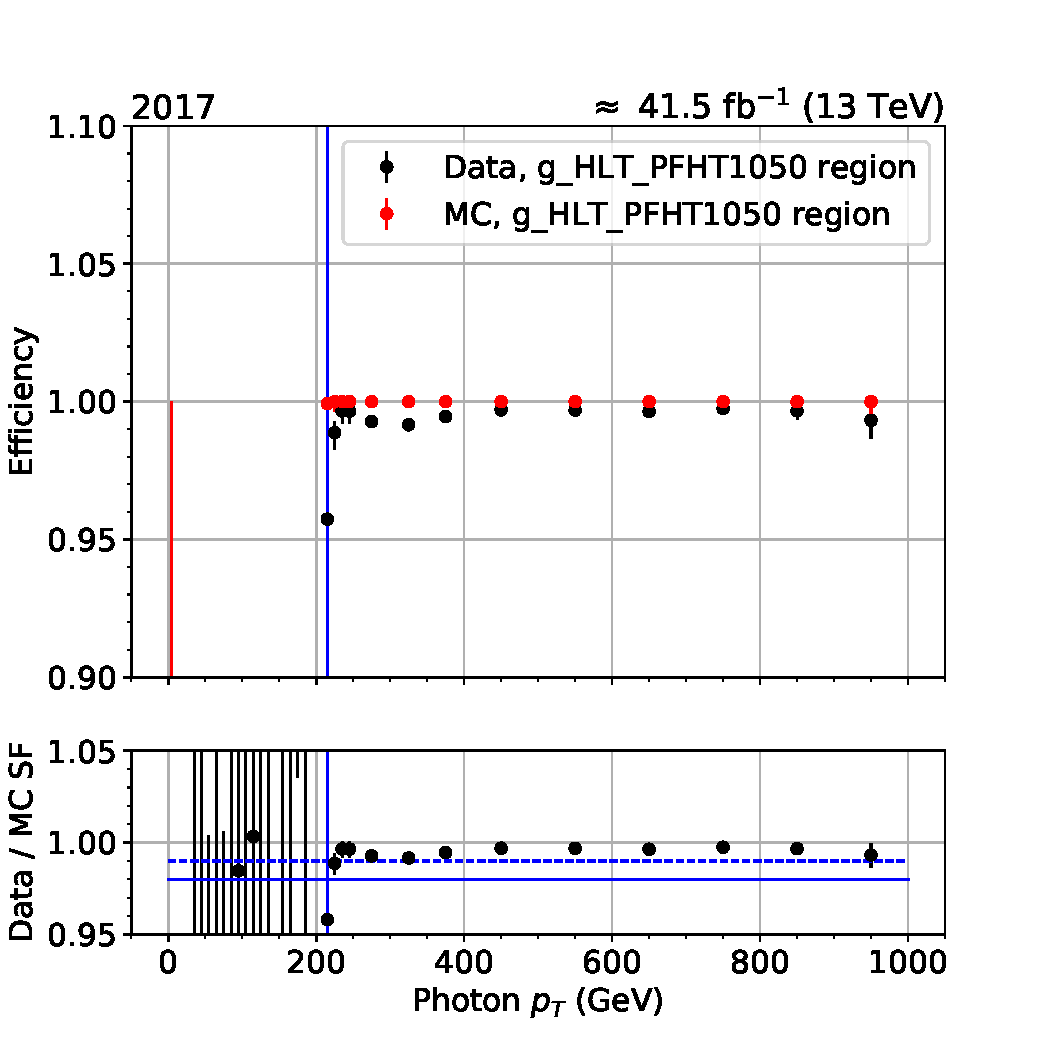
\includegraphics[width=0.49\textwidth]{fig/efficiency/trigger/photon/data_mc_comparison_g_HLT_PFHT1050_2017.pdf}
    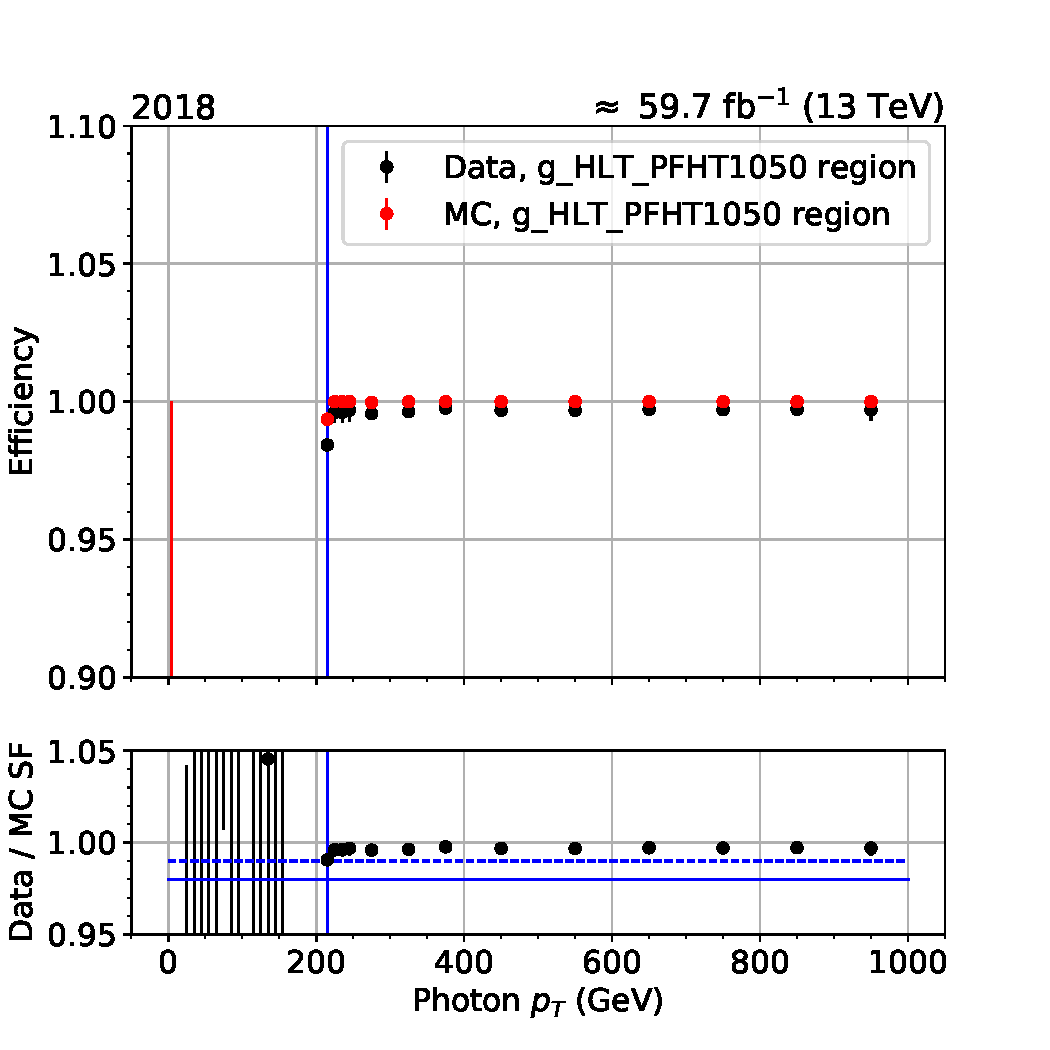
\includegraphics[width=0.49\textwidth]{fig/efficiency/trigger/photon/data_mc_comparison_g_HLT_PFHT1050_2018.pdf}
    \caption{Efficiency of the \texttt{HLT\_Photon200} trigger in data (black) and \HT-binned \texttt{GJets} simulation (red) for 2017 (left) and 2018 (right) as a function of photon \pt. The bottom panel shows the MC-to-data efficiency scale factor. The blue vertical line indicates a photon \pt of $215~\GeV$, which is the requirement used in the analysis selection.}
    \label{fig:hlteff_photon}
 \end{center}\end{figure*}

\subsubsection{Electron trigger}
{\color{red} We also need to add information about the single electron trigger efficiencies}

\subsection{Pileup reweighting}

The pileup (PU) conditions in the simulated samples are not identical to the ones observed measured in data, and a reweighting is applied to remove the difference.
The reweighting is performed by matching the true pileup distribution of each simulated sample
with the pileup distribution in data, obtained through the pileupCalc tool
assuming a minimum bias cross section of 69.2$\pm 4.6\%$~mb, following the recommendations in in Ref.~\cite{pileup_twiki}. The true pileup distributions in data and simulation are shown in Fig.~\ref{fig:purwg_true}. The distribution of the number of reconstructed vertices for $W\to \mu\nu$ events before and after PU reweighting is shown in Fig.~\ref{fig:purwt_npv}. In this variable, the PU reweighting method leads to a worse overall agreement between data and simulation. To check this behavior, the distribution of the event energy density $\rho$ is shown in Fig.~\ref{fig:purwt_npv}, again before and after PU reweighting. Here, the agreement before PU reweighting is worse than in the primary vertex distribution and the PU reweighting clearly improves the agreement.

\begin{figure}[ht!]
  \begin{center}
    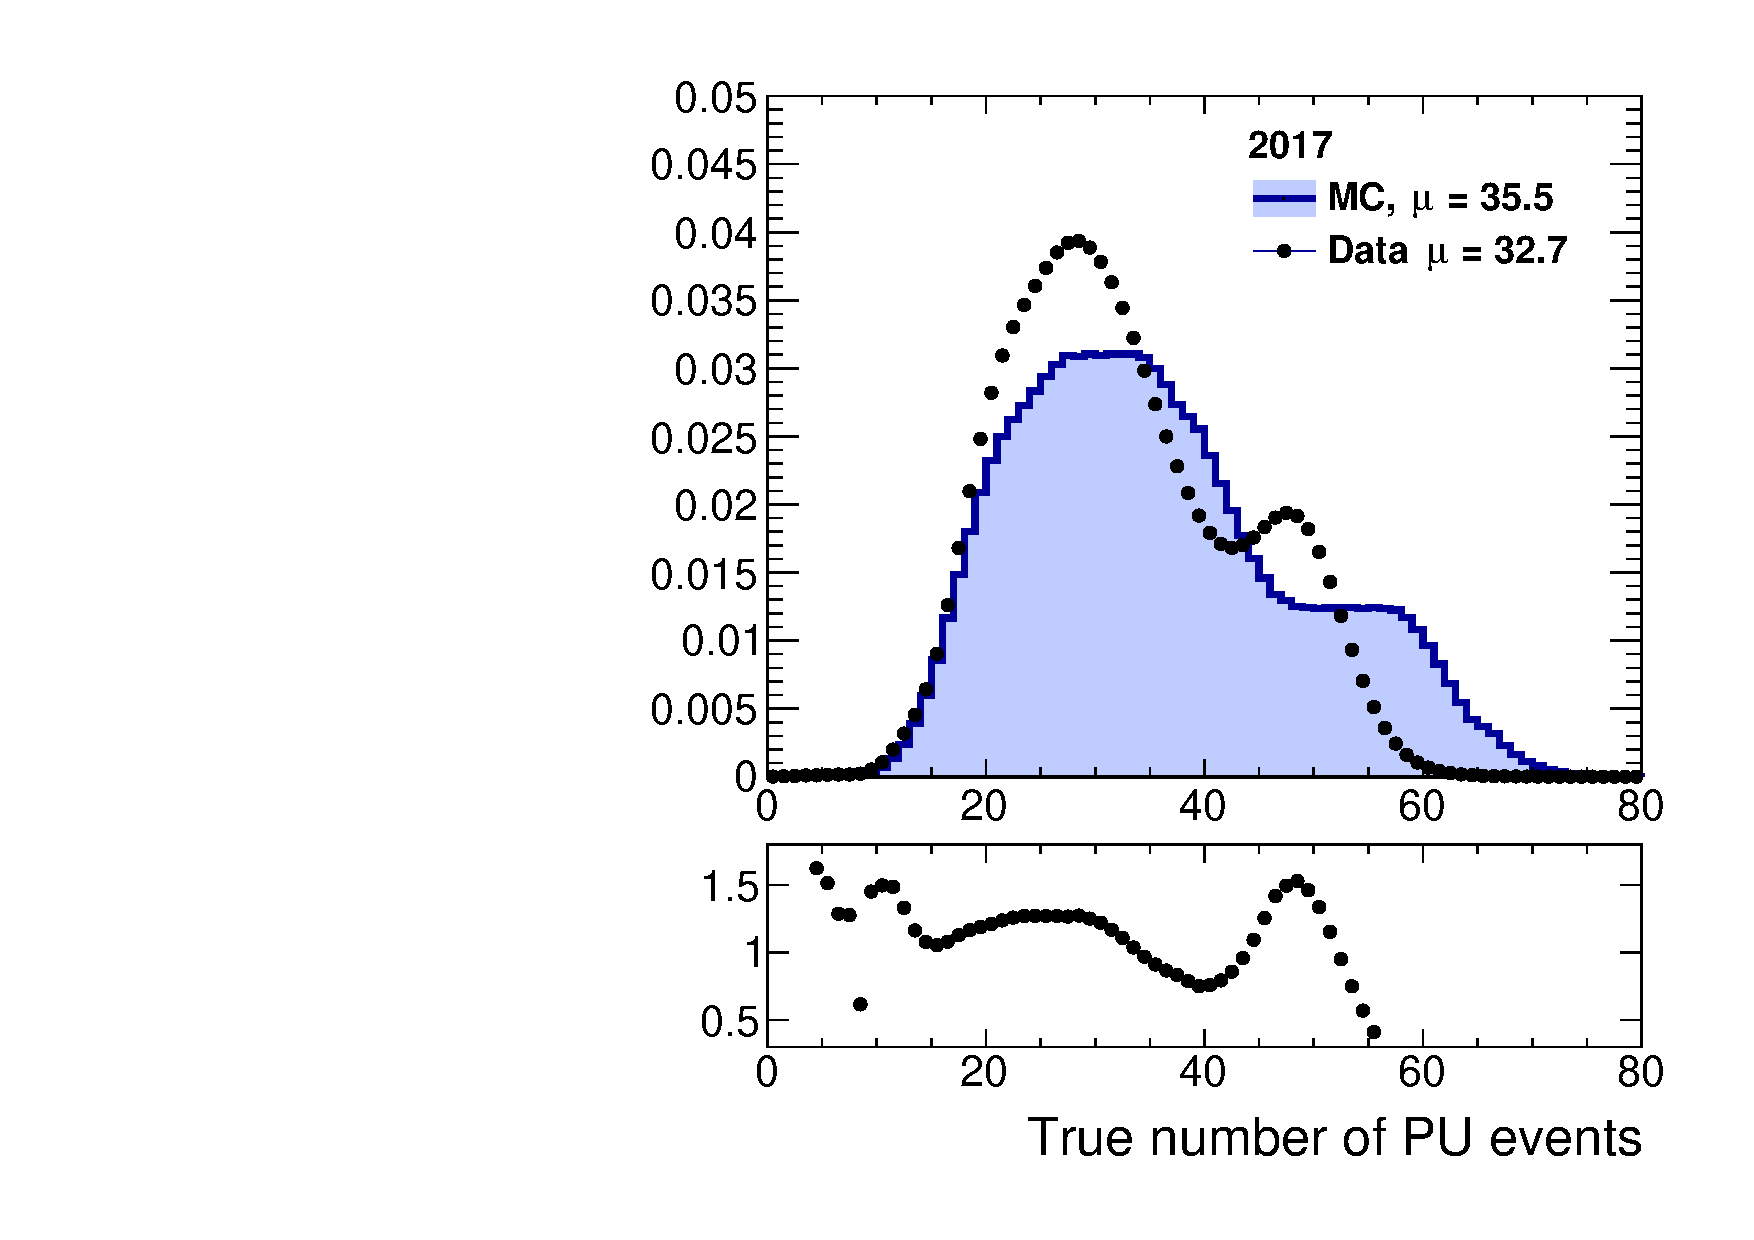
\includegraphics[width=0.49\textwidth]{fig/pileup/pu_weights_2017.pdf}
    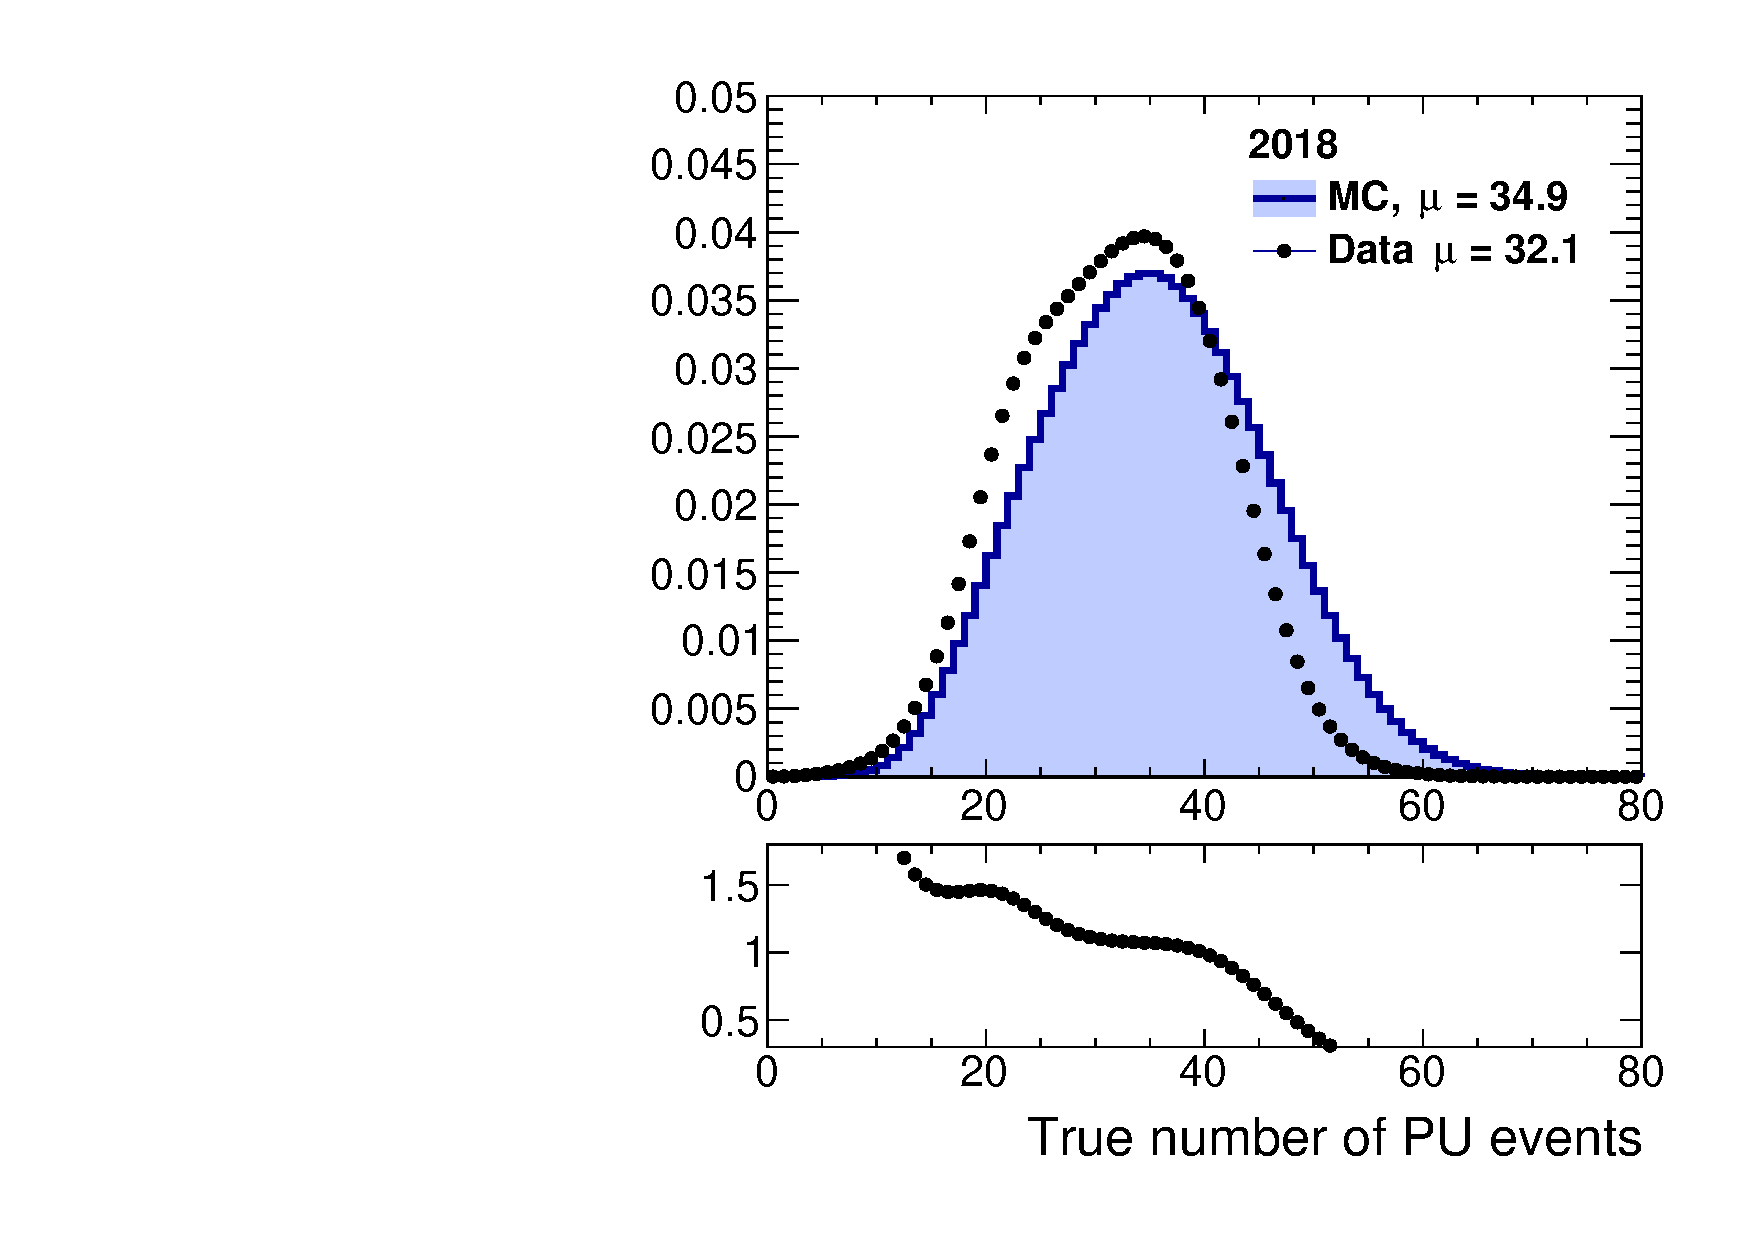
\includegraphics[width=0.49\textwidth]{fig/pileup/pu_weights_2018.pdf}
    \caption{
        Distribution of the true number of PU events in data and simulation for 2017 (left) and 2018 (right).
        The distributions for data are extracted assuming a minimum bias cross section of $69.2~\mathrm{mb}$.
    }
    \label{fig:purwg_true}
  \end{center}
\end{figure}
\begin{figure}[ht!]
  \begin{center}
    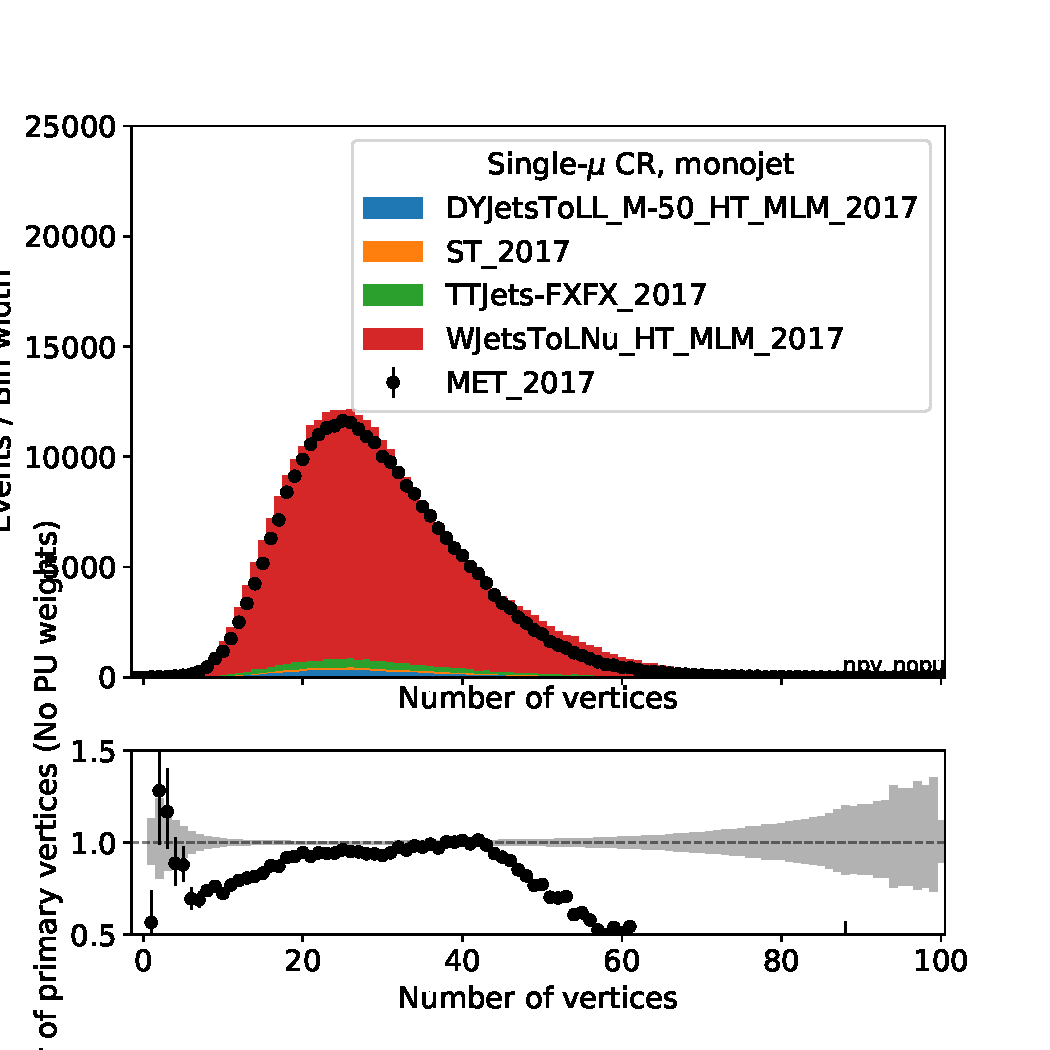
\includegraphics[width=0.49\textwidth]{fig/pileup/cr_1m_j_npv_nopu_2017.pdf}
    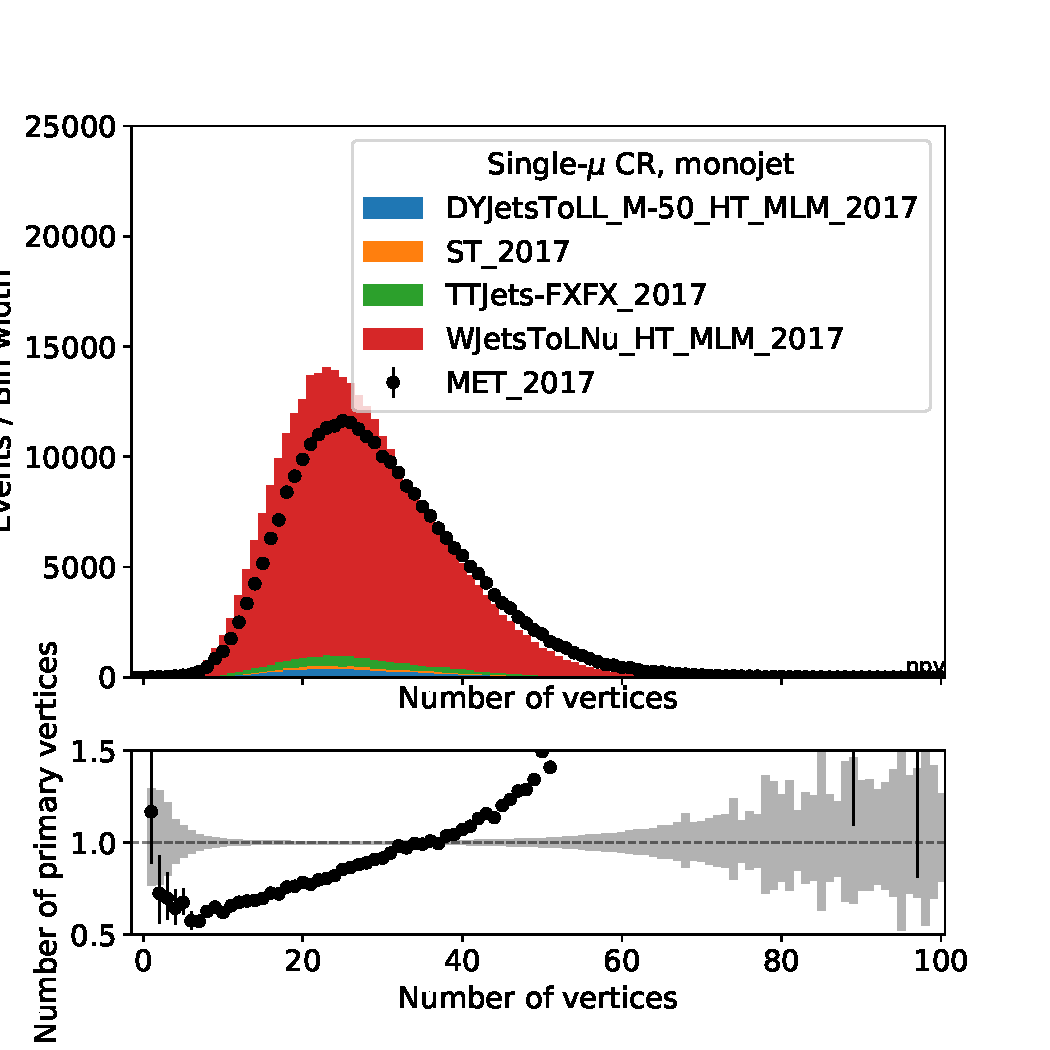
\includegraphics[width=0.49\textwidth]{fig/pileup/cr_1m_j_npv_2017.pdf}
    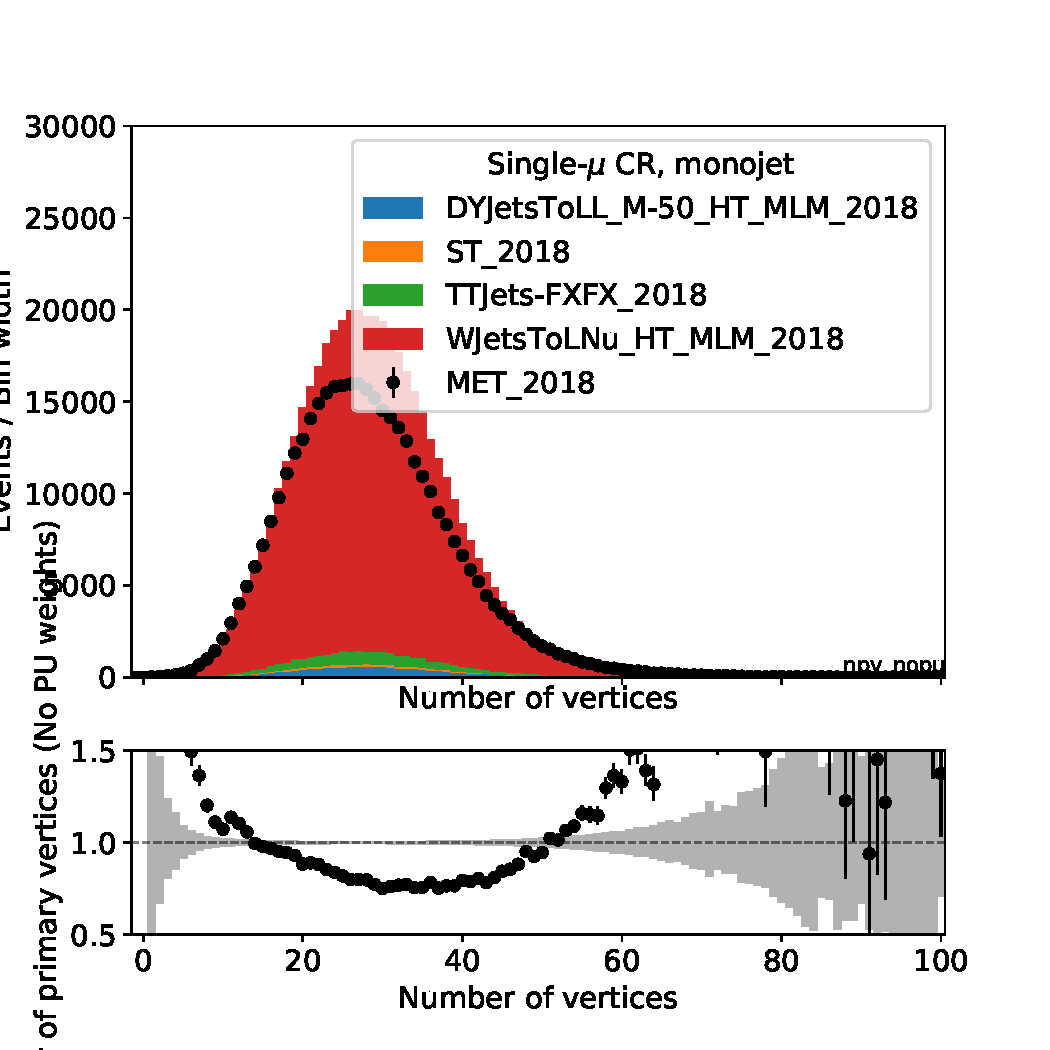
\includegraphics[width=0.49\textwidth]{fig/pileup/cr_1m_j_npv_nopu_2018.pdf}
    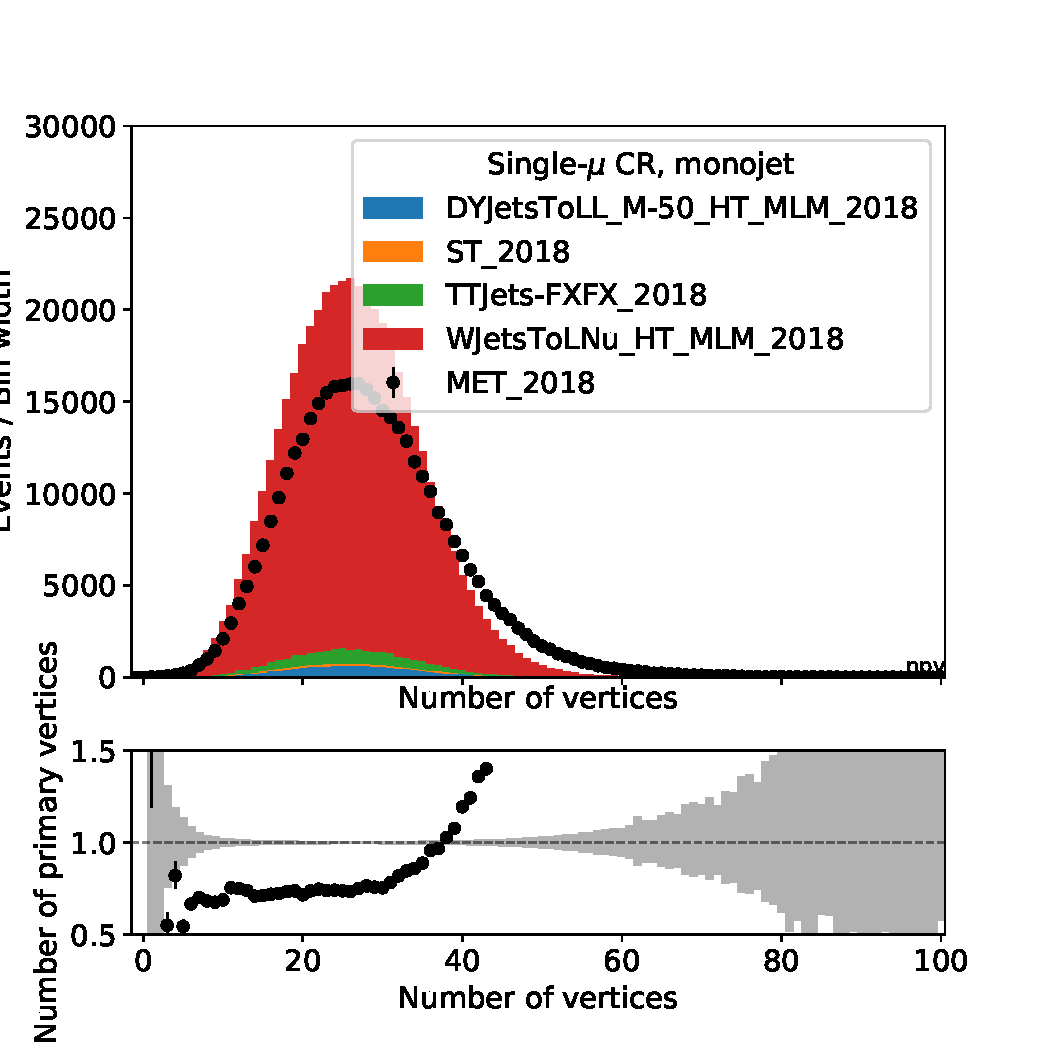
\includegraphics[width=0.49\textwidth]{fig/pileup/cr_1m_j_npv_2018.pdf}
    \caption{
        Distribution of the number of vertices in \Wmn~events in data and
        simulation before pileup re-weighting (left) and after pileup reweighting (right).
        The Monte Carlo is normalized to the luminosity of 41.53 and 59.7 fb$^{-1}$, respectively for 2017 and 2018.
    }
    \label{fig:purwt_npv}
  \end{center}
\end{figure}
\begin{figure}[ht!]
  \begin{center}
    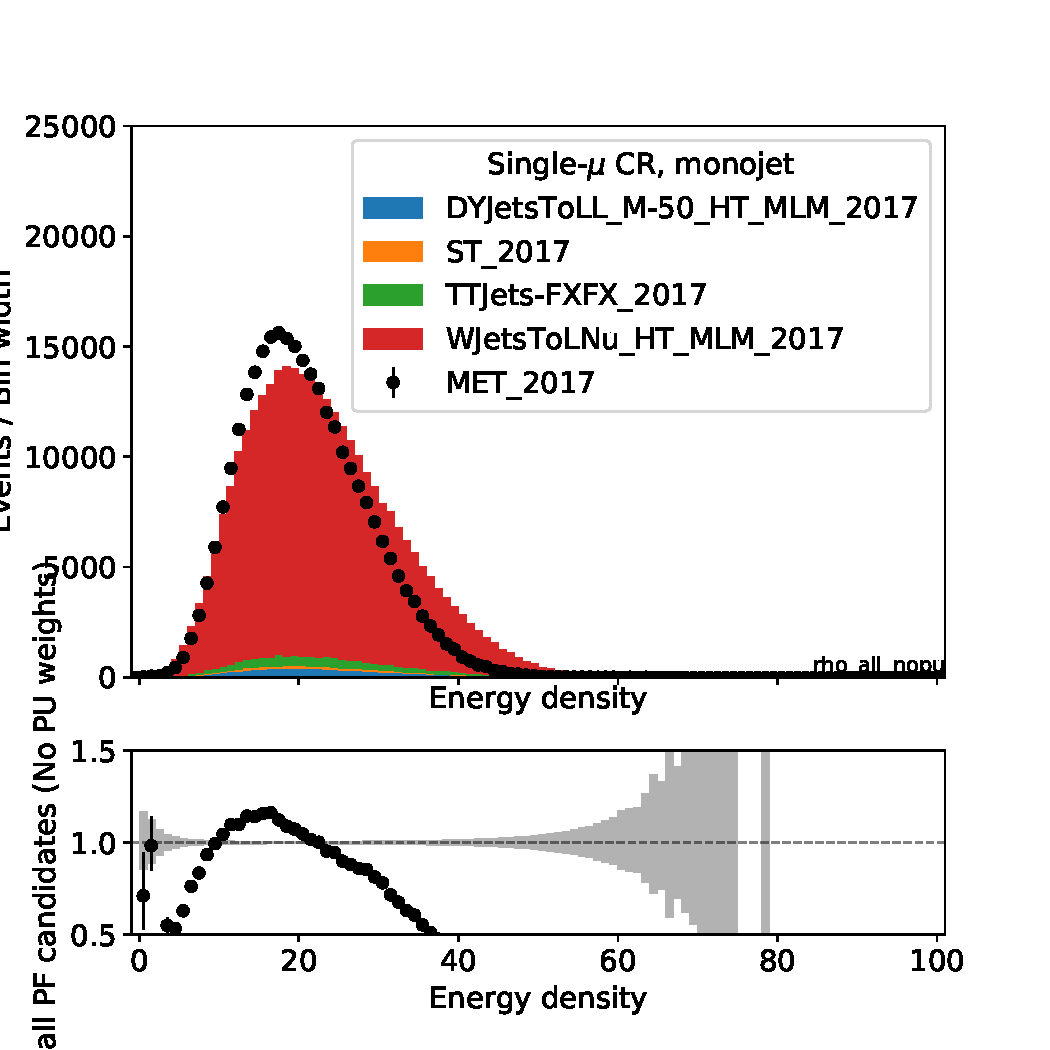
\includegraphics[width=0.49\textwidth]{fig/pileup/cr_1m_j_rho_all_nopu_2017.pdf}
    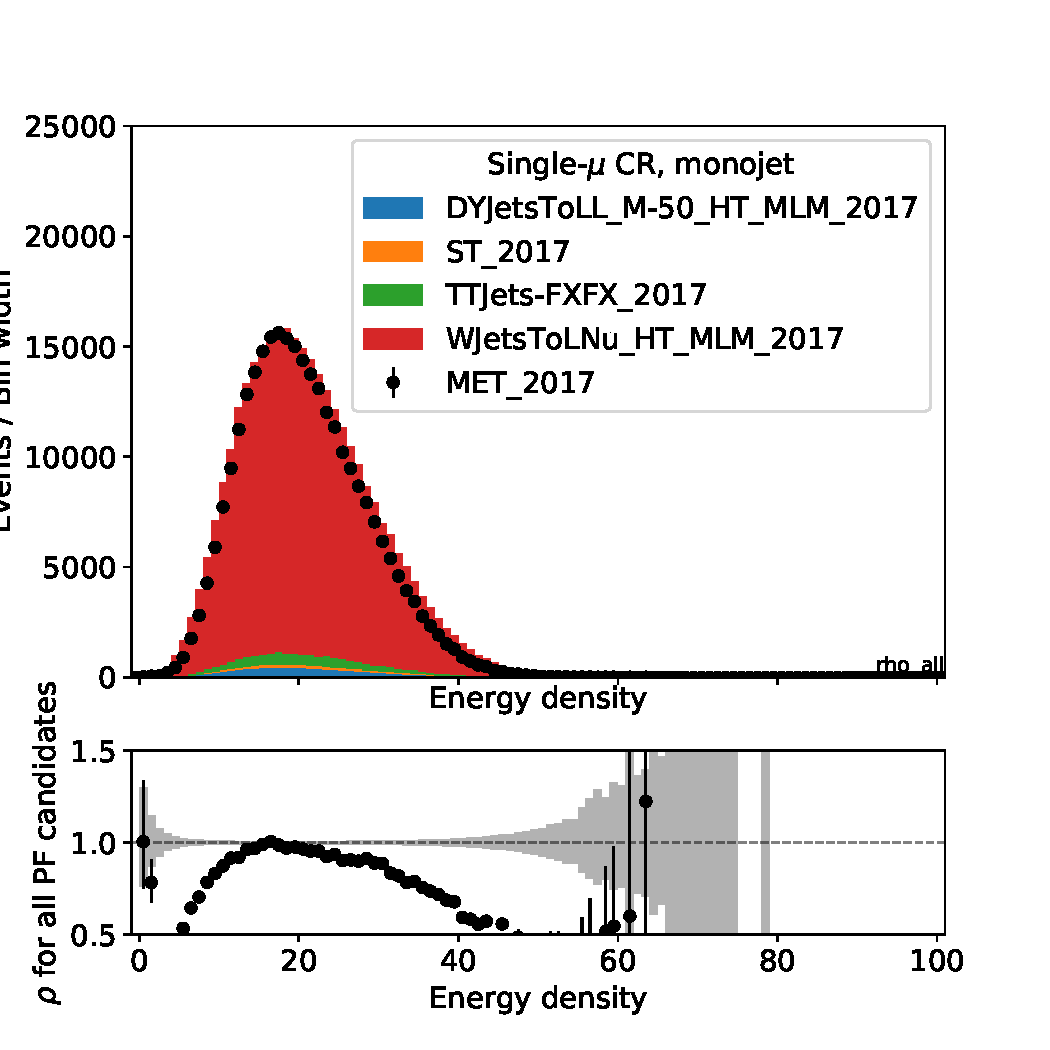
\includegraphics[width=0.49\textwidth]{fig/pileup/cr_1m_j_rho_all_2017.pdf}
    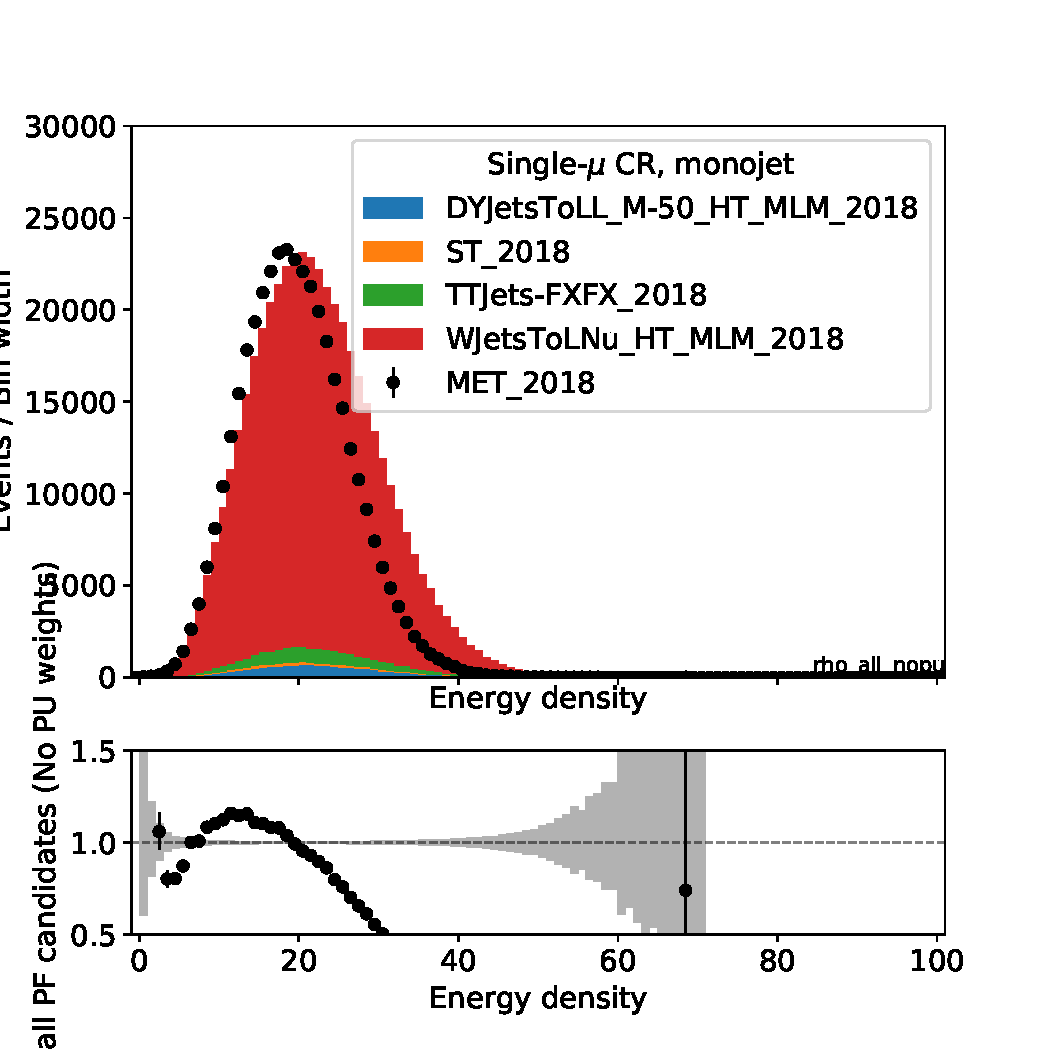
\includegraphics[width=0.49\textwidth]{fig/pileup/cr_1m_j_rho_all_nopu_2018.pdf}
    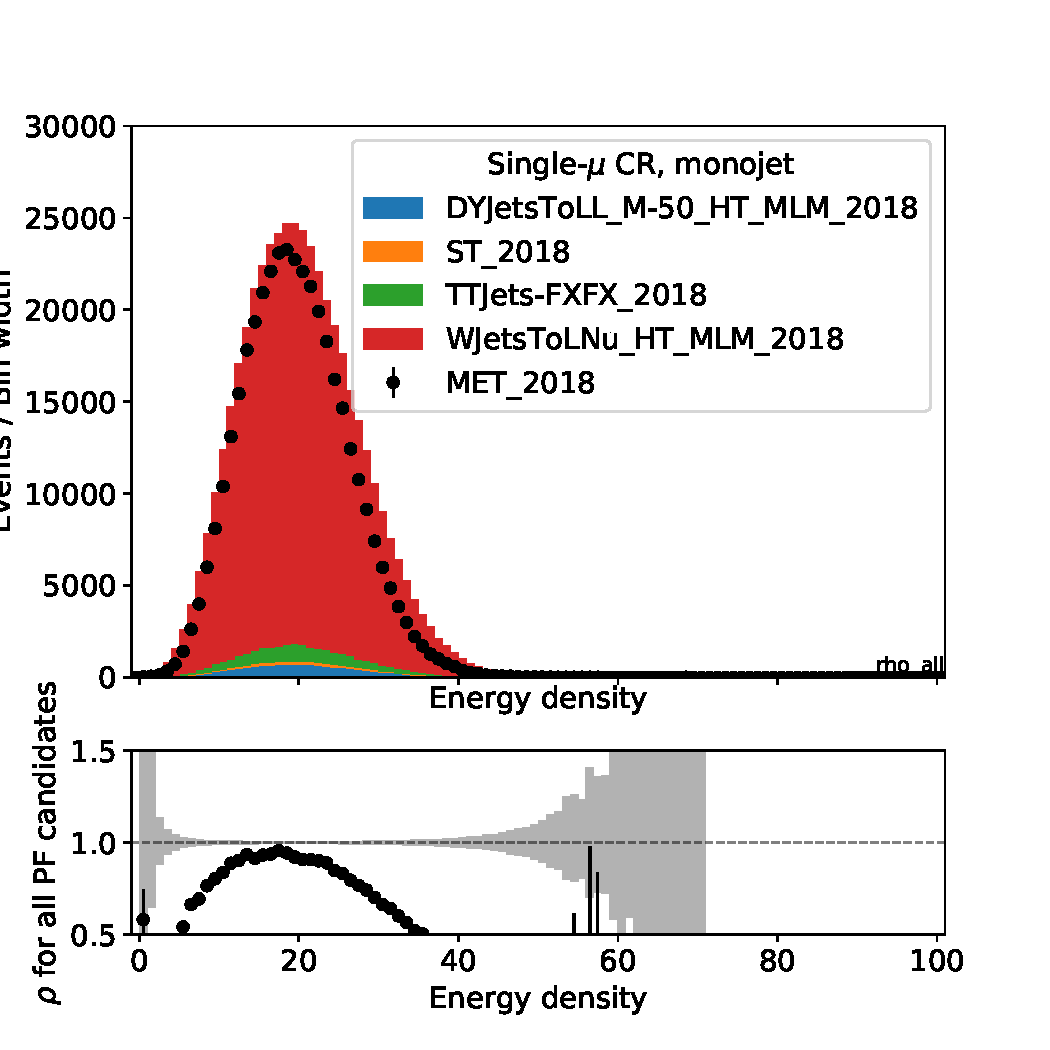
\includegraphics[width=0.49\textwidth]{fig/pileup/cr_1m_j_rho_all_2018.pdf}
    \caption{
        Distribution of the event energy density $\rho$  in \Wmn~events in data and
        simulation before pileup re-weighting (left) and after pileup reweighting (right).
        The Monte Carlo is normalized to the luminosity of 41.53 and 59.7 fb$^{-1}$, respectively for 2017 and 2018.
    }
    \label{fig:purwt_rho}
  \end{center}
\end{figure}

\subsection{Lepton and photon identification/reconstruction efficiency reweighting}

Data-to-simulation scale factors are applied to events in the control regions to
account for differences in the reconstruction, identification and isolation of leptons
between data and simulationn. These data-to-MC scale factors are derived from the efficiencies that are measured for the electron and muon
selections in bins of $\pt$ and $\eta$ in both data and simulation. These scale factors are
provided by the relevant POGs.


The reconstruction scale factors for electrons are shown in Fig.~\ref{fig:sf_electron_reco}. The corresponding identification scale factors for veto and tight electrons are shown in Fig.~\ref{fig:sf_electron_id}, and include the effect of the isolation efficiency. 

The identification scale factors for muons are shown in Fig.~\ref{fig:sf_muon_id}. Here, isolation scale factors are applied separately and are shown in Fig.~\ref{sf_muon_iso}. The corresponding corrections for muons are deemed negligible~\cite{CMS-MUO-TWIKI-SF}.

\begin{figure}[ht!]
  \begin{center}
    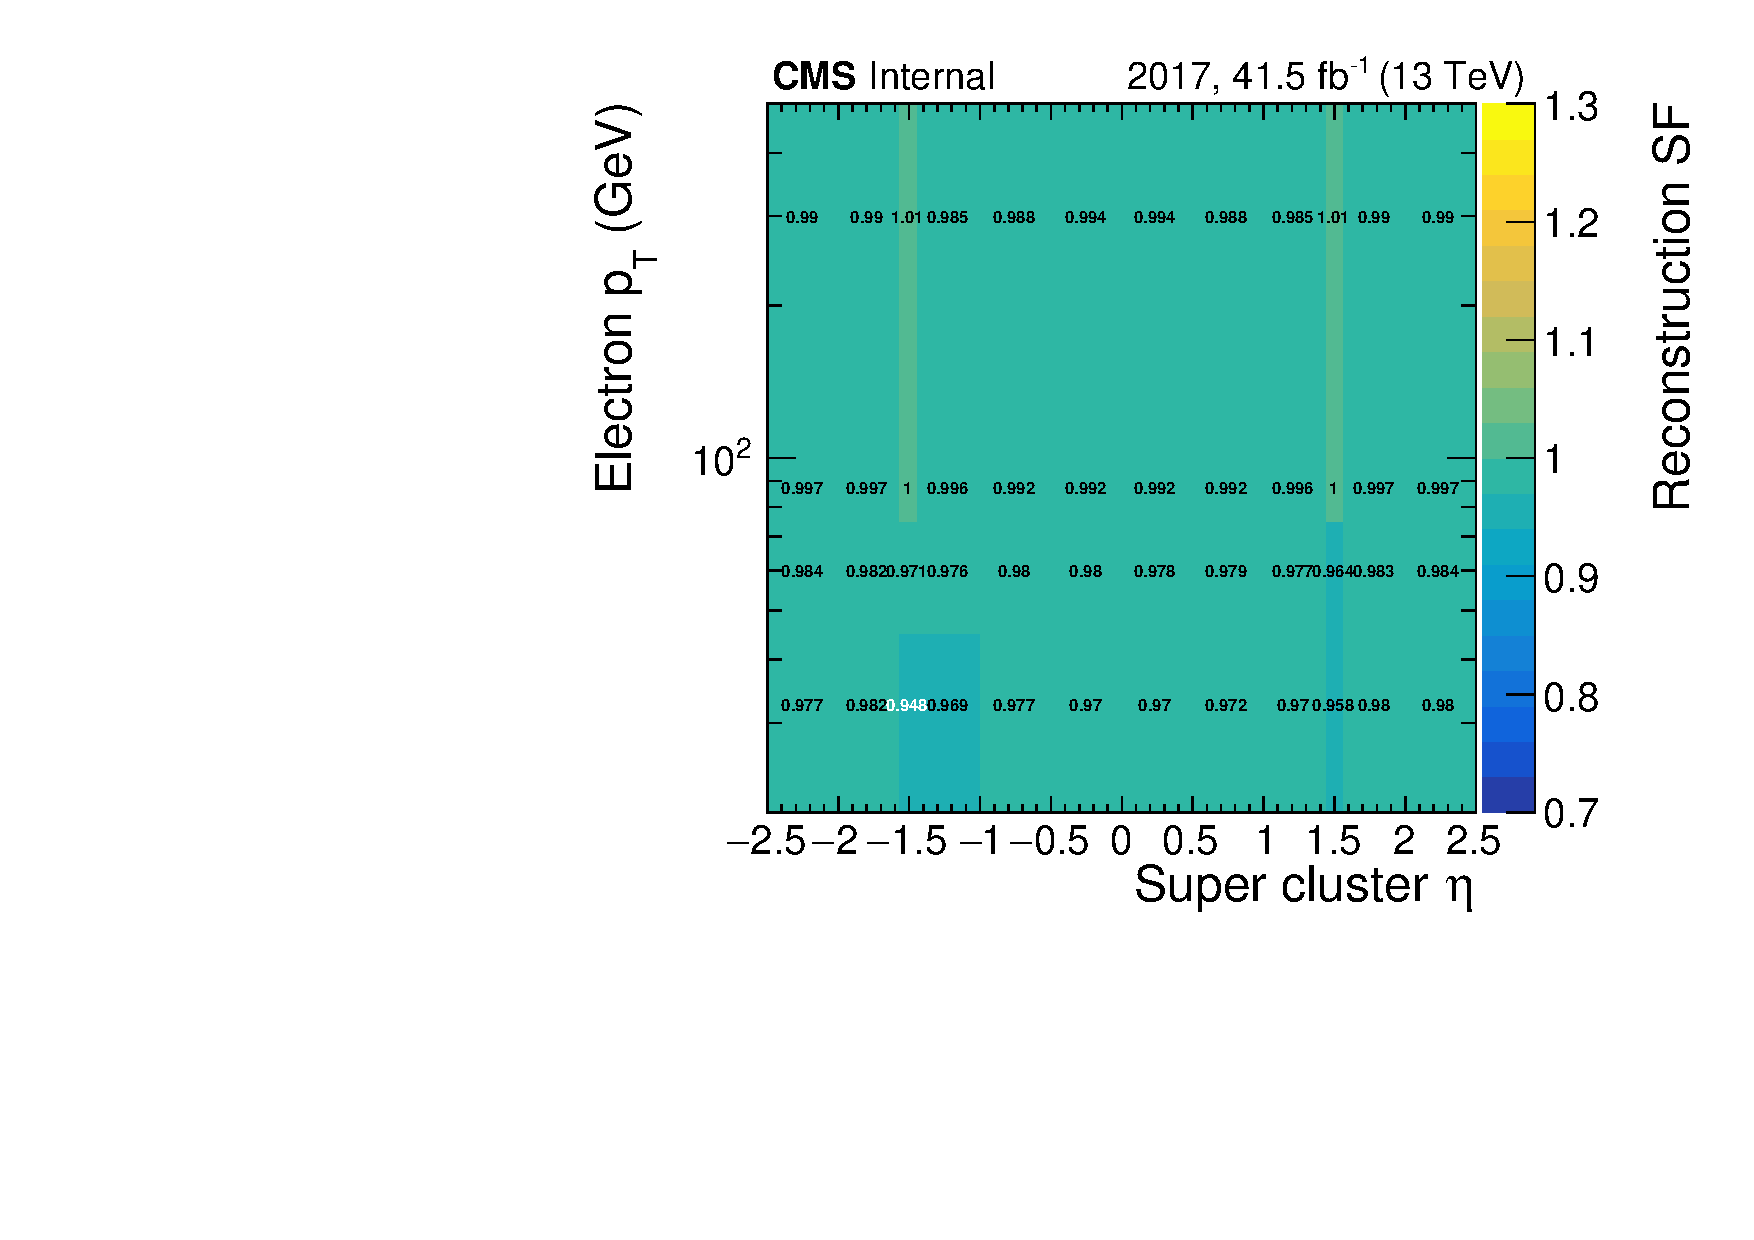
\includegraphics[width=0.49\textwidth]{fig/efficiency/lepton/ele_eff_reco_2017.pdf}
    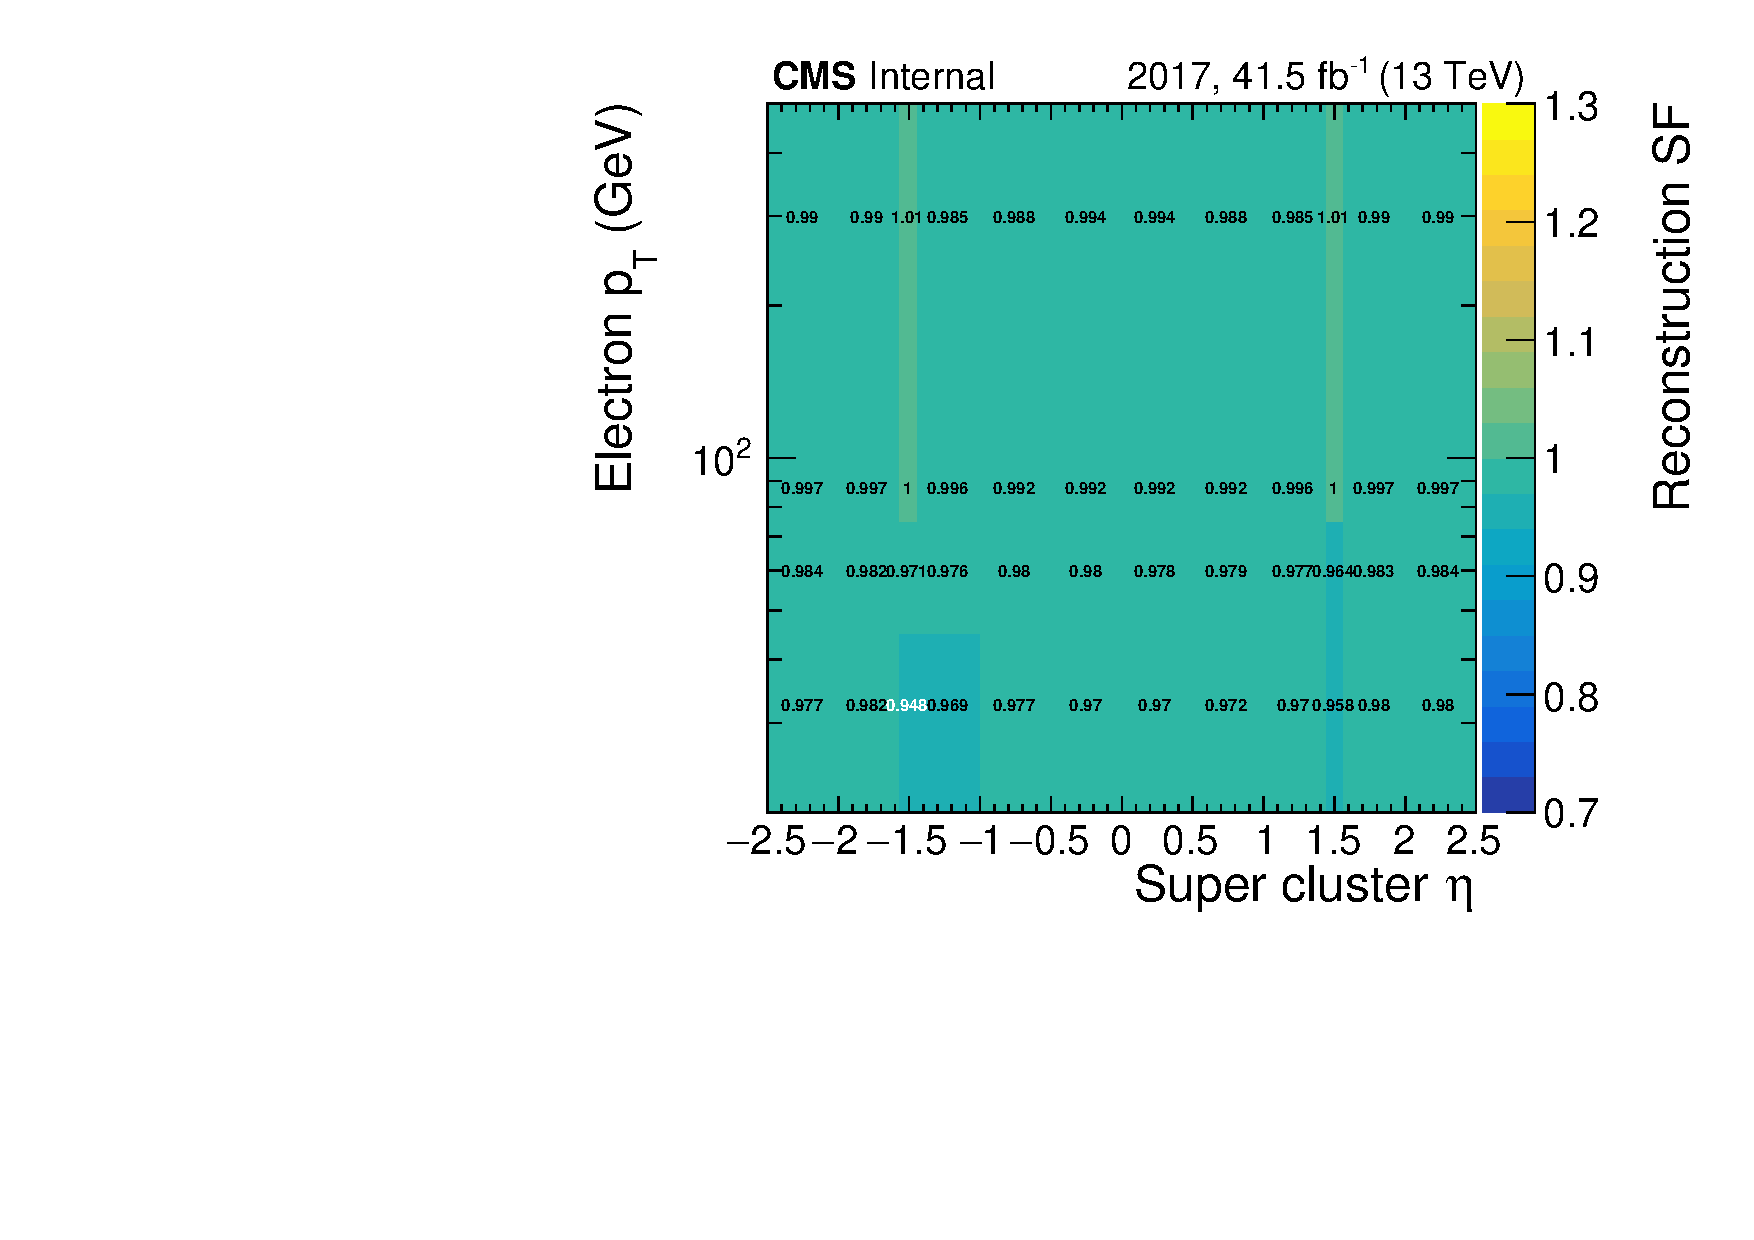
\includegraphics[width=0.49\textwidth]{fig/efficiency/lepton/ele_eff_reco_2017.pdf}\\
    \caption{
      Scale factors for the reconstruction efficiency of electrons starting from a super cluster for 2017 (left) and 2018(right)
    }
    \label{fig:sf_electron_reco}
  \end{center}
\end{figure}
\begin{figure}[ht!]
  \begin{center}
    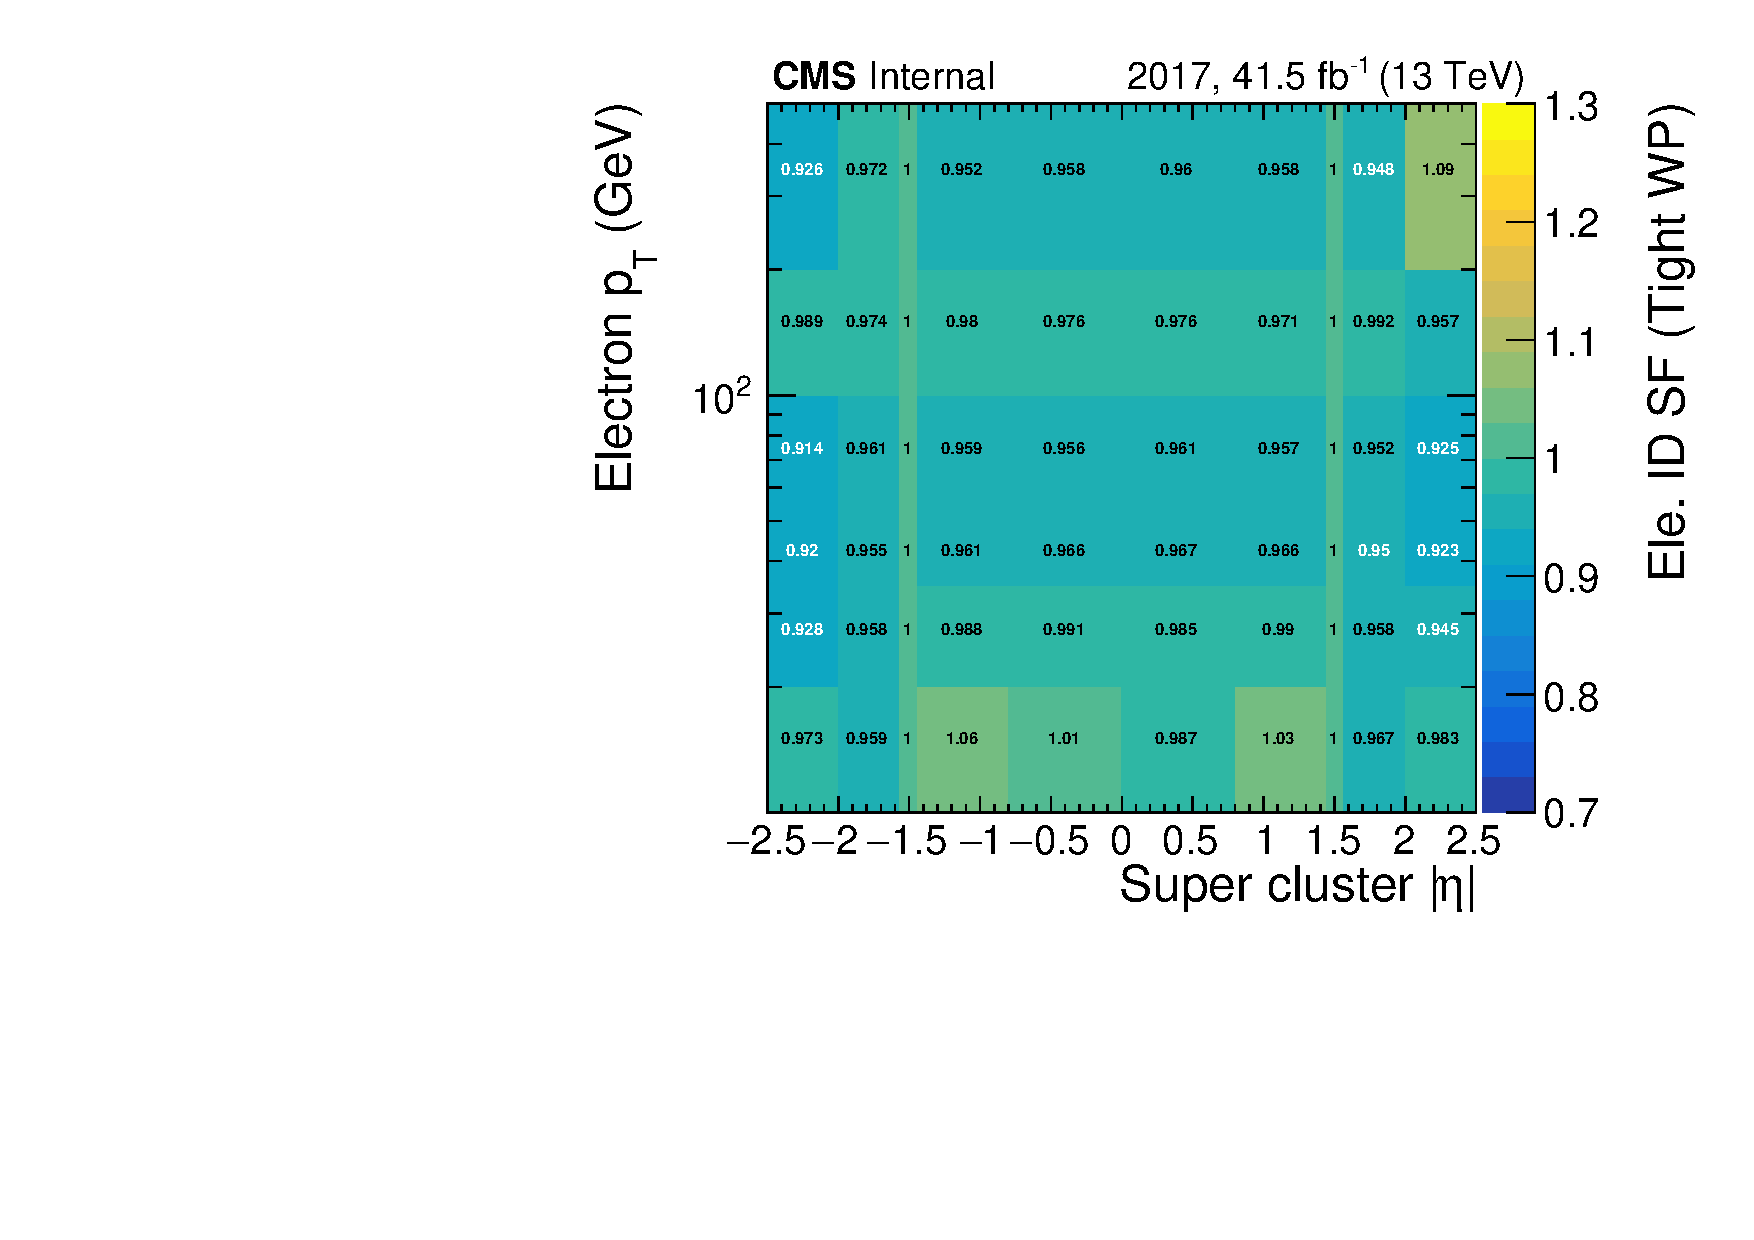
\includegraphics[width=0.49\textwidth]{fig/efficiency/lepton/ele_eff_tight_id_2017.pdf}
    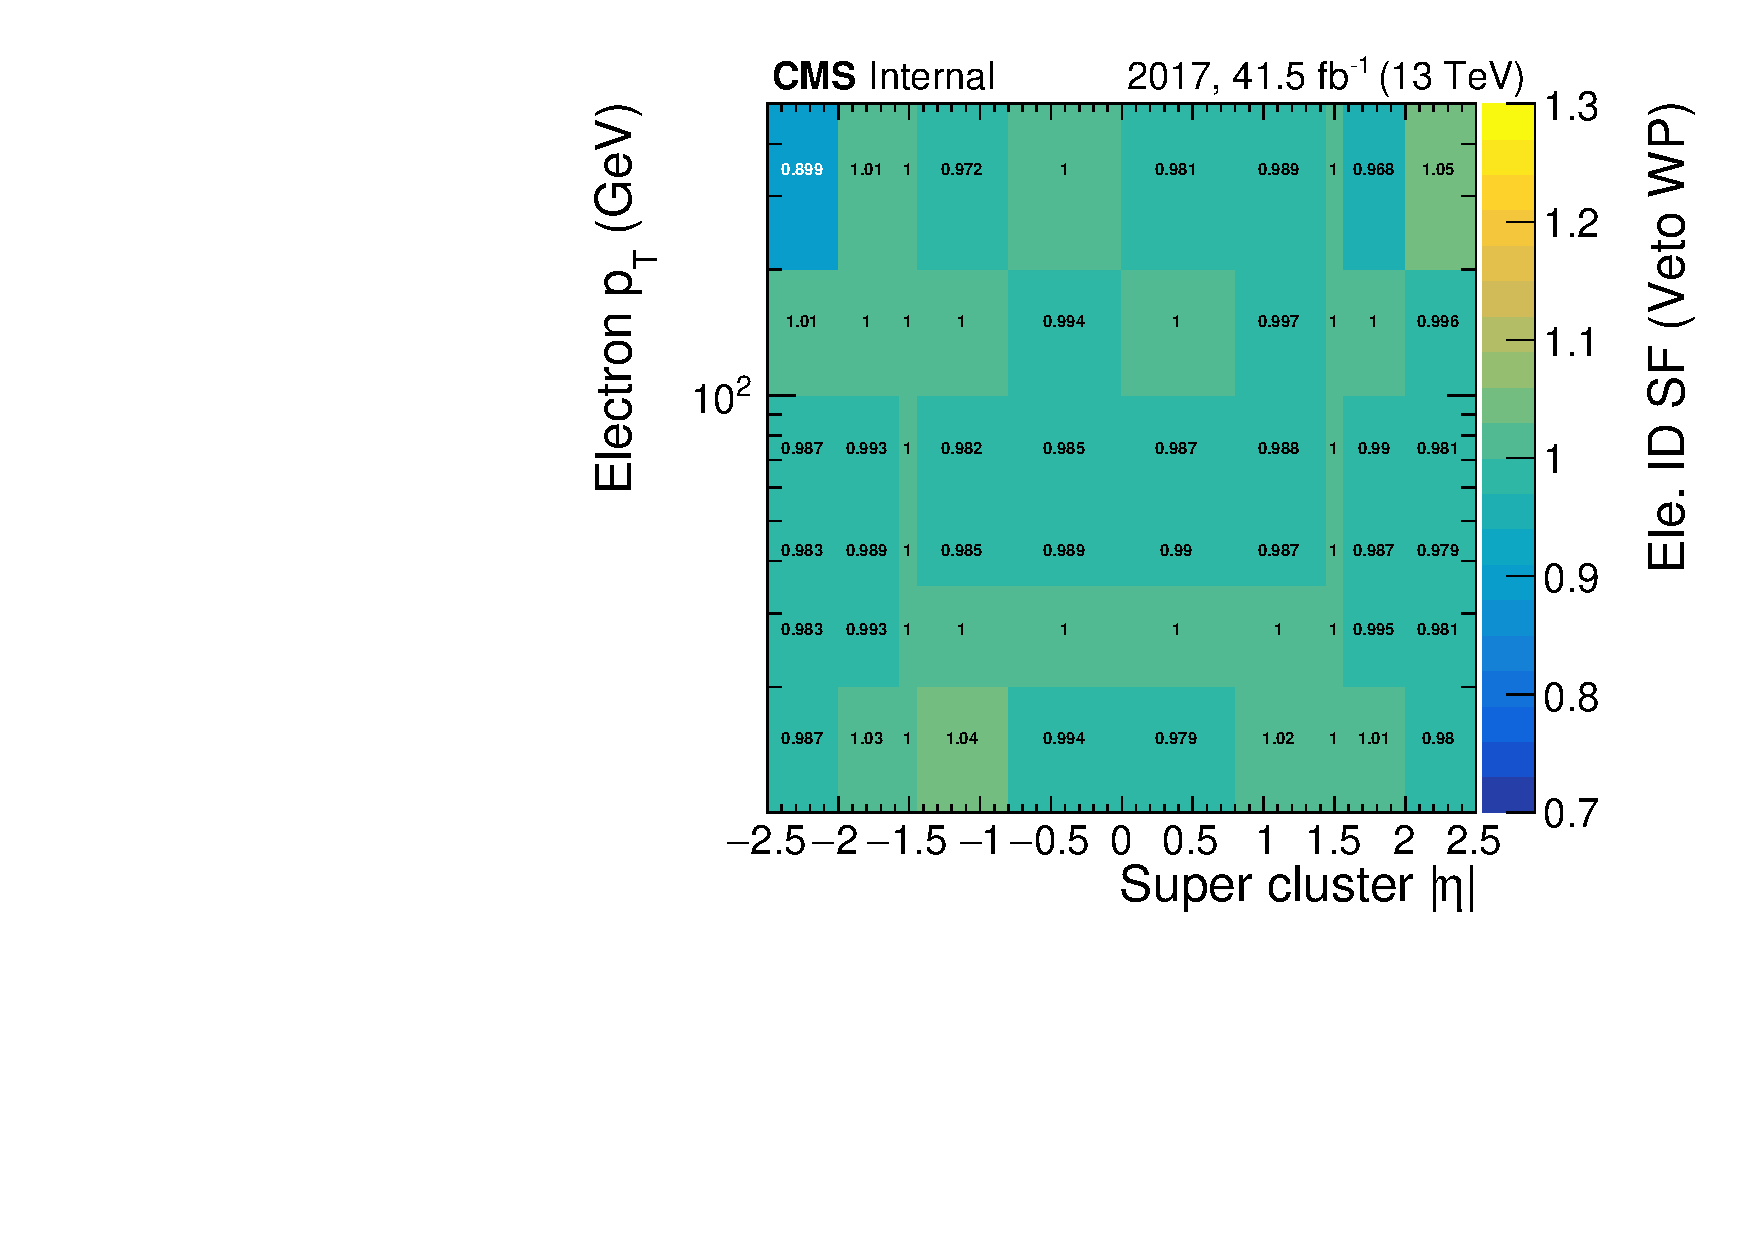
\includegraphics[width=0.49\textwidth]{fig/efficiency/lepton/ele_eff_loose_id_2017.pdf}\\
    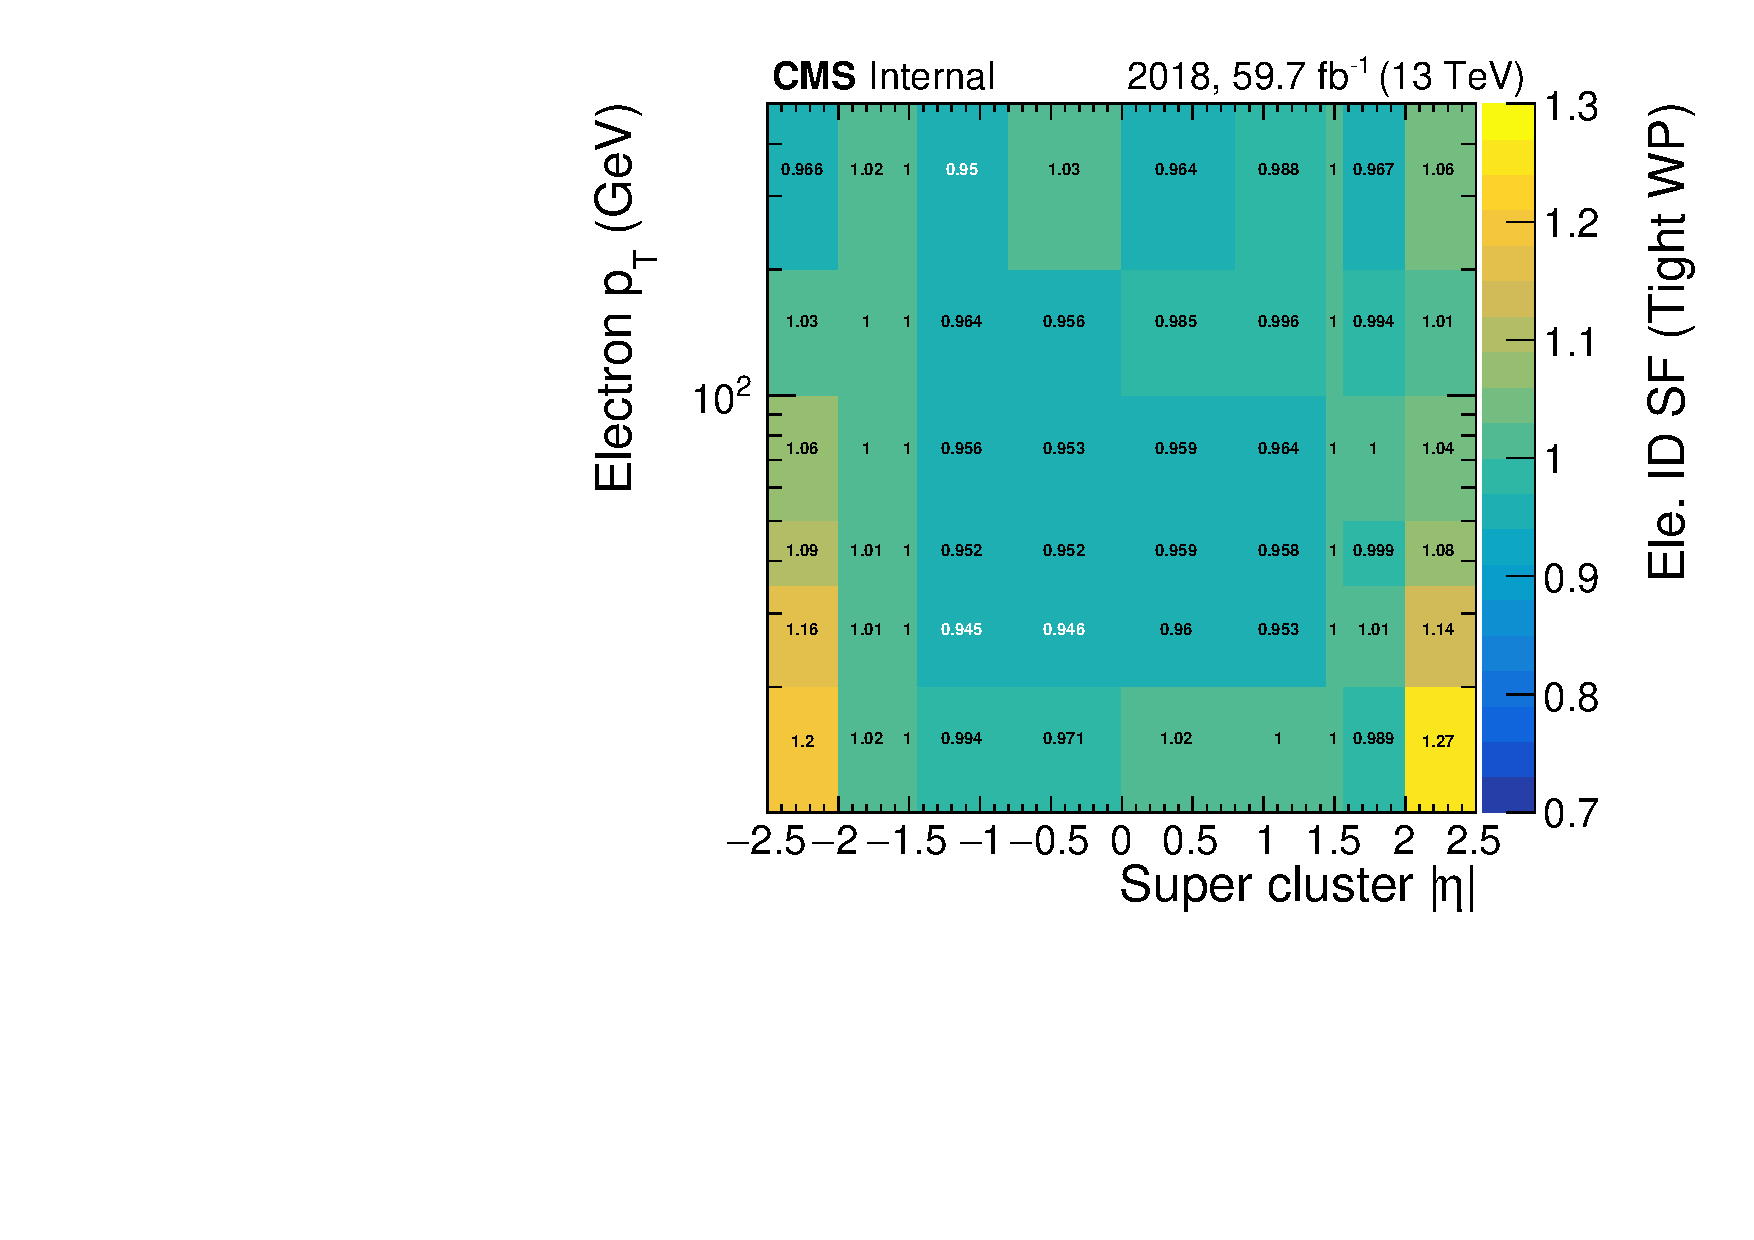
\includegraphics[width=0.49\textwidth]{fig/efficiency/lepton/ele_eff_tight_id_2018.pdf}
    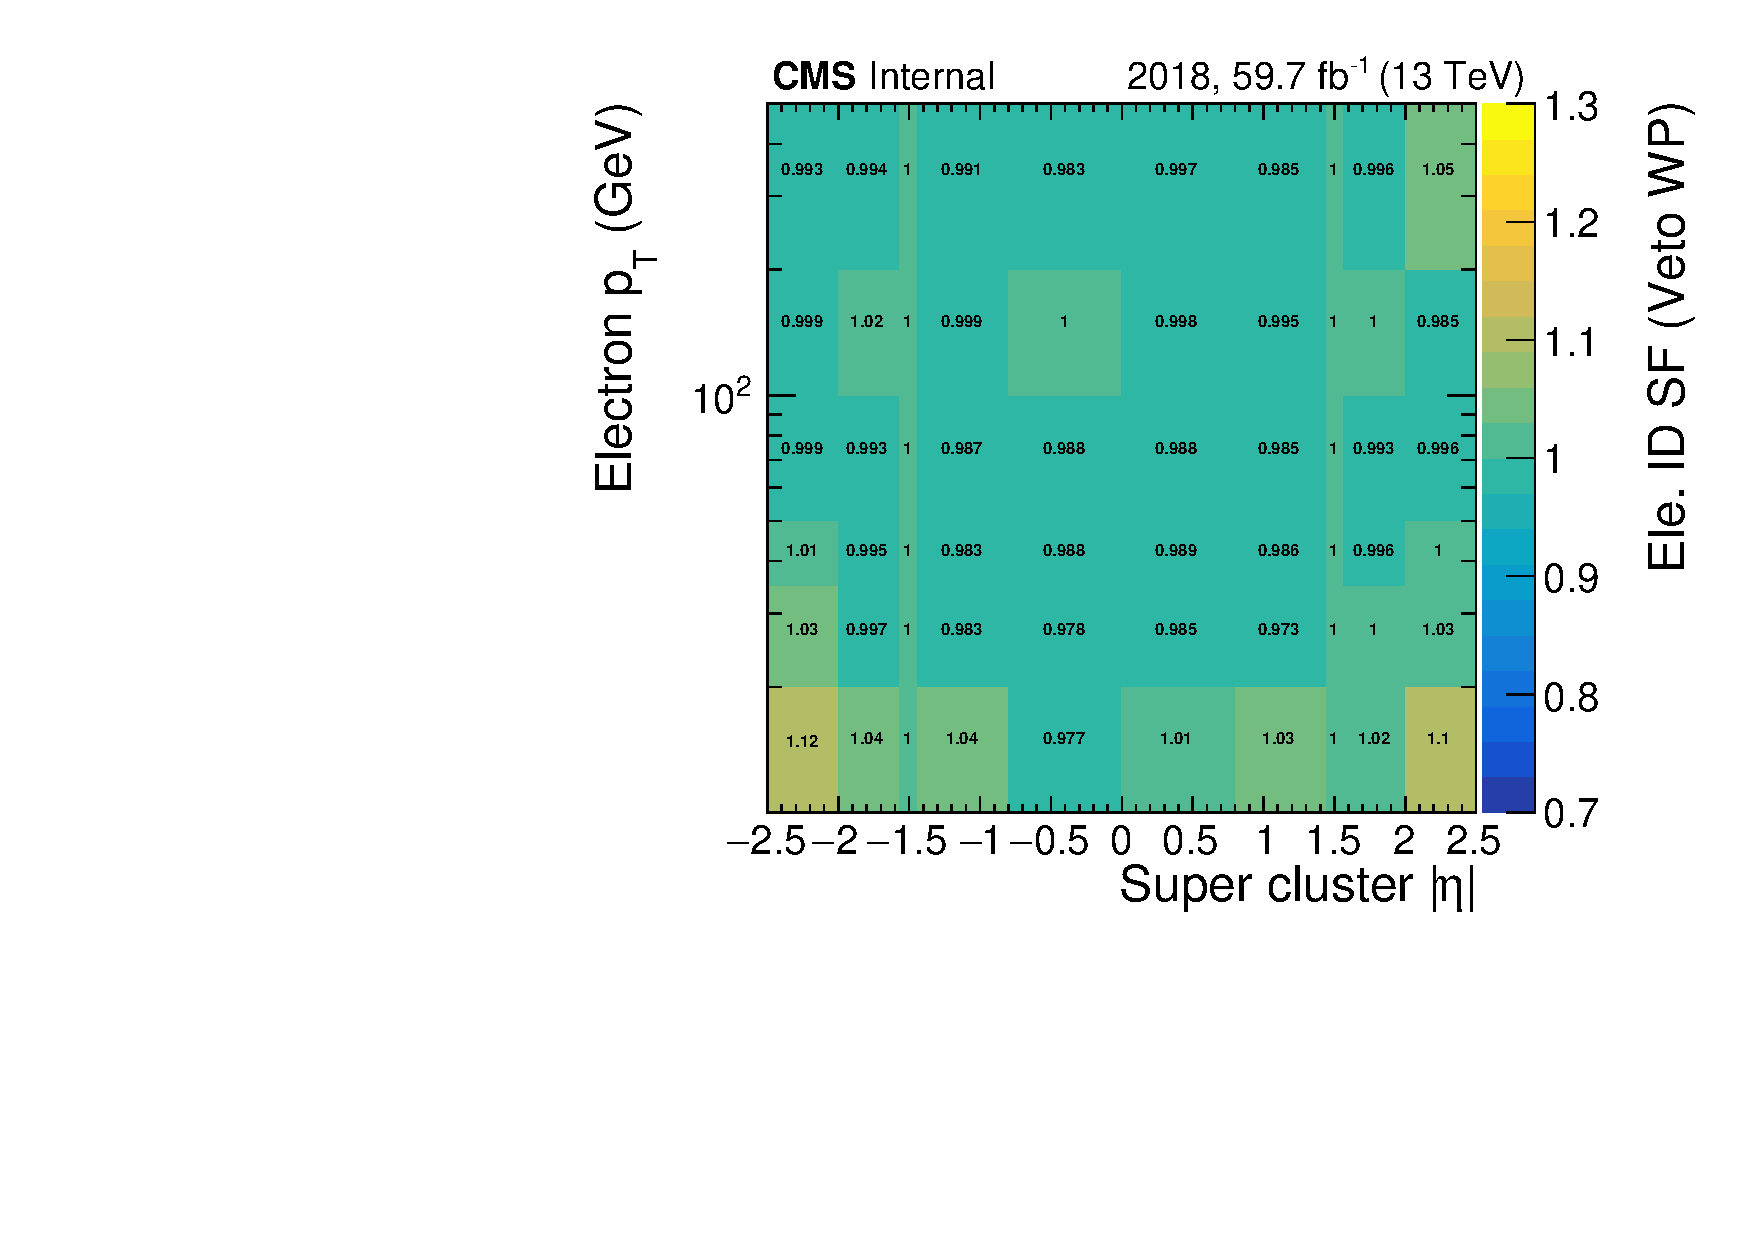
\includegraphics[width=0.49\textwidth]{fig/efficiency/lepton/ele_eff_loose_id_2018.pdf}
    \caption{
      Scale factors for tight (left) and veto (right) electrons are shown for 2017 (top) and
      2018 (bottom). The scale factors are provided in bins of electron $\pt$ and $\eta$.
    }
    \label{fig:sf_electron_id}
  \end{center}
\end{figure}

The scale factors for id and isolation for tight muons are shown in Fig.~\ref{fig:sfmuon}.

\begin{figure}[ht!]
  \begin{center}
    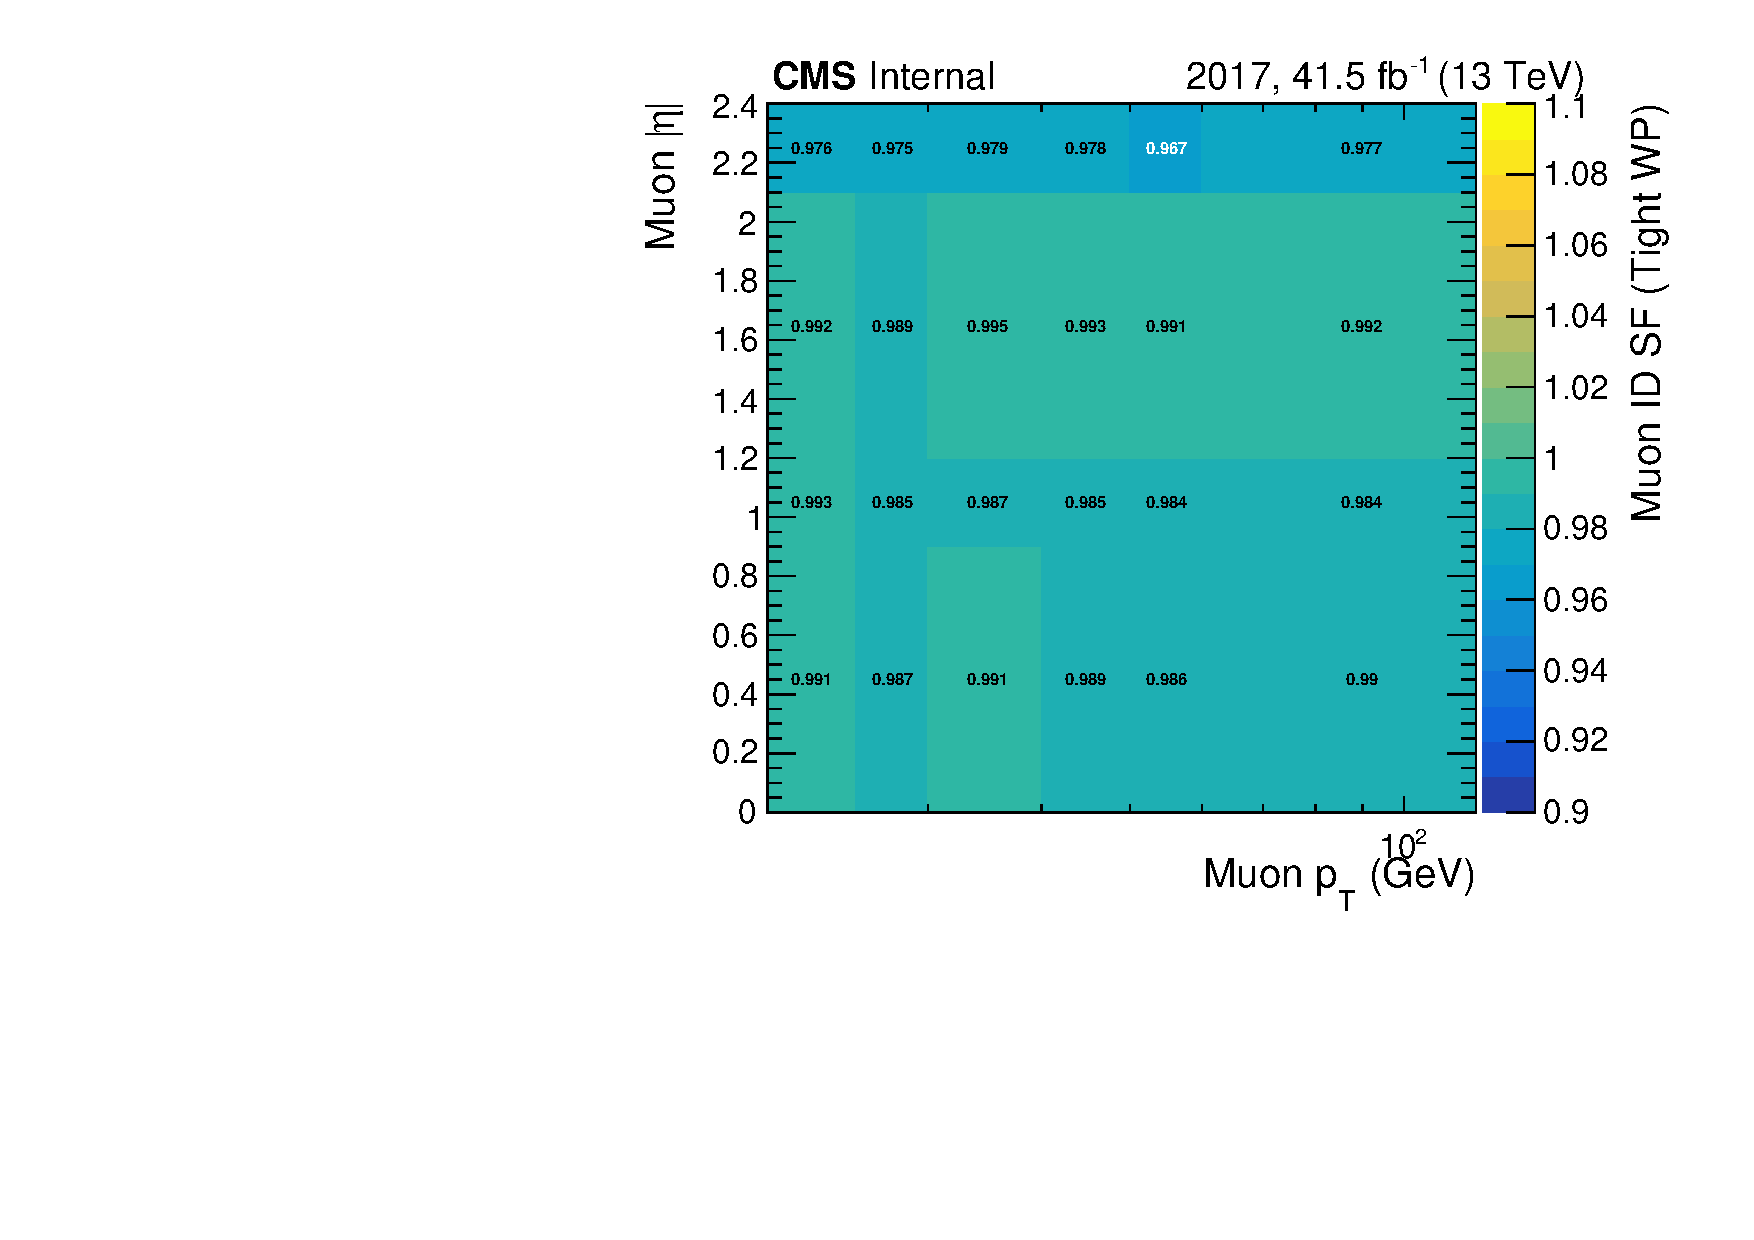
\includegraphics[width=0.49\textwidth]{fig/efficiency/lepton/muon_eff_tight_id_2017.pdf}
    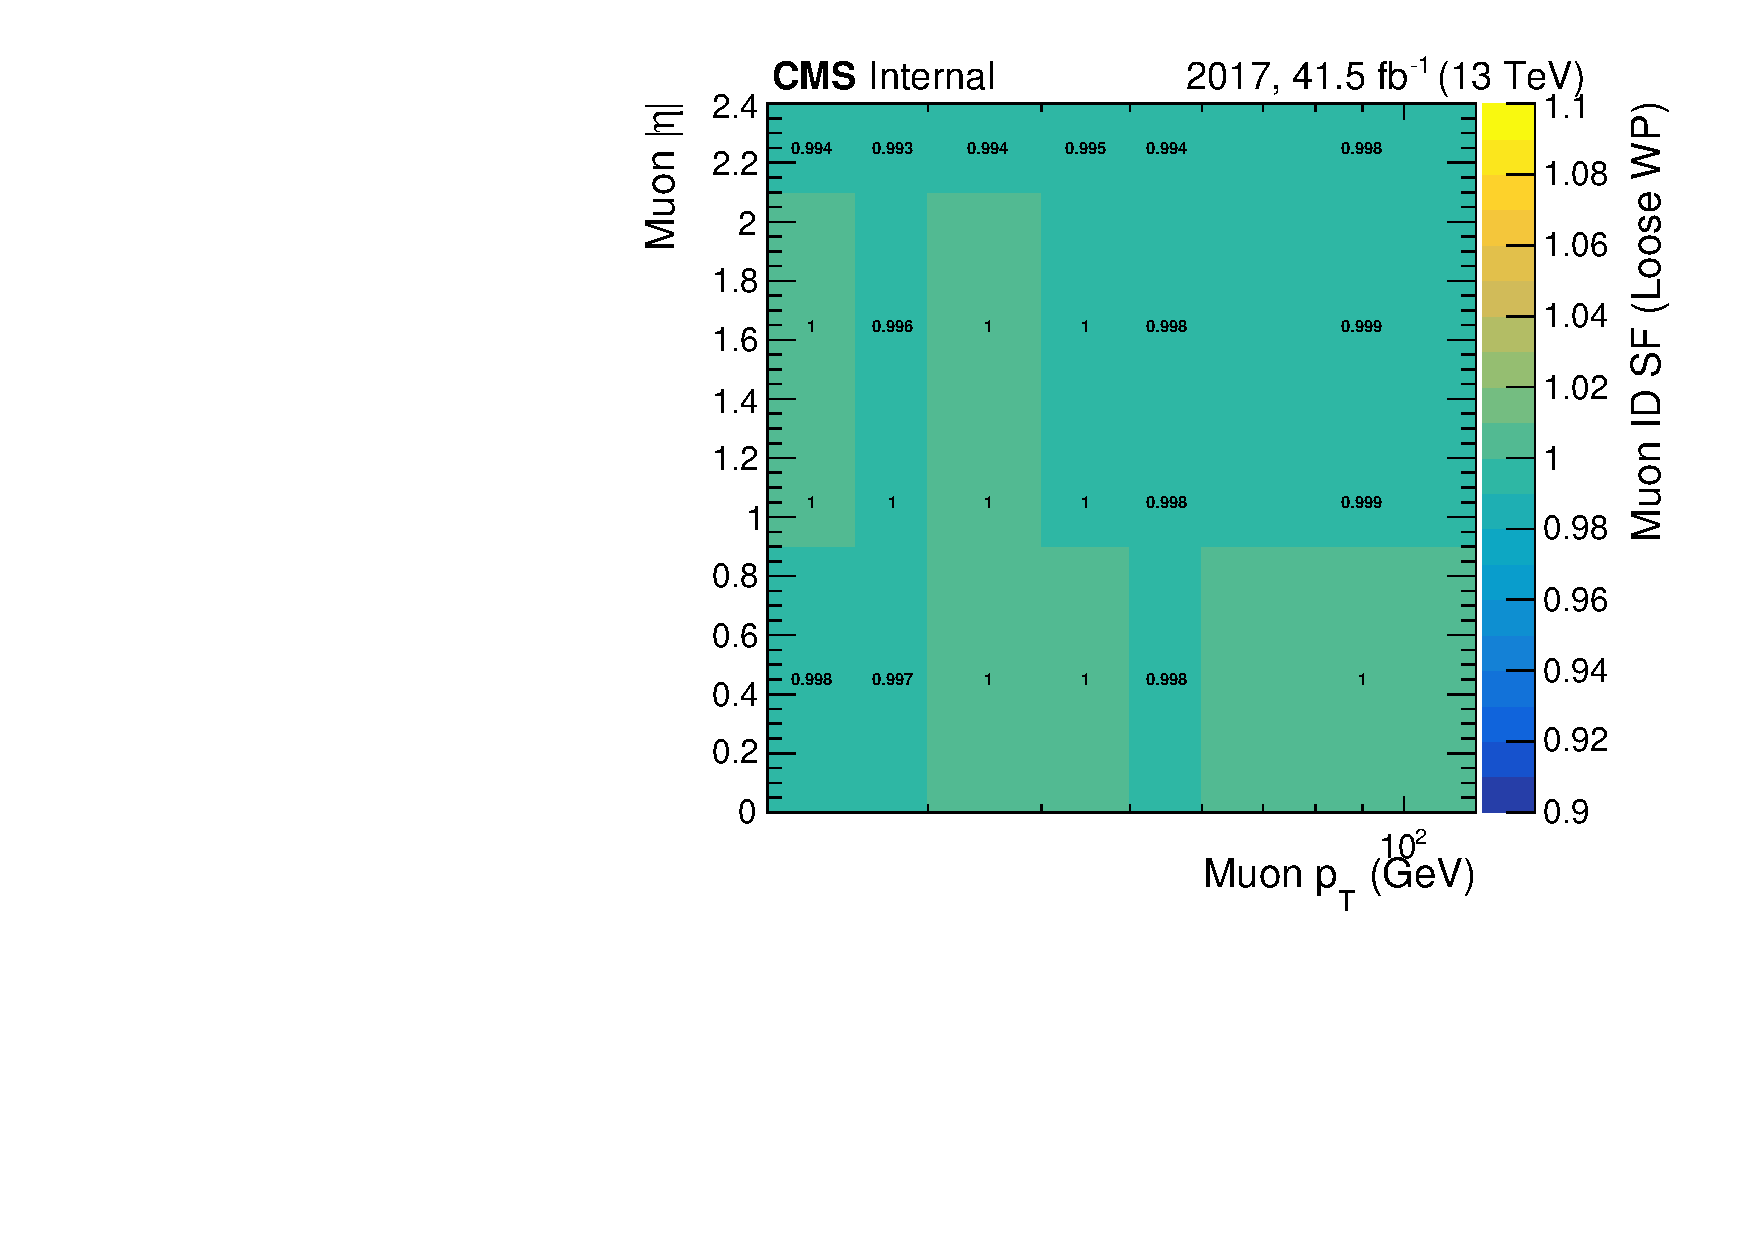
\includegraphics[width=0.49\textwidth]{fig/efficiency/lepton/muon_eff_loose_id_2017.pdf}\\
    \includegraphics[width=0.49\textwidth]{fig/efficiency/lepton/muon_eff_tight_id_2018.pdf}
    \includegraphics[width=0.49\textwidth]{fig/efficiency/lepton/muon_eff_loose_id_2018.pdf}
    \caption{
      Scale factors for tight (left) and veto (right) muon identification are shown for 2017 (top) and
      2018 (bottom). The scale factors are provided in bins of electron $\pt$ and $\eta$.
    }
    \label{fig:sf_muon_id}
  \end{center}
\end{figure}


\begin{figure}[ht!]
    \begin{center}
        \includegraphics[width=0.49\textwidth]{fig/efficiency/lepton/muon_eff_tight_iso_2017.pdf}
        \includegraphics[width=0.49\textwidth]{fig/efficiency/lepton/muon_eff_loose_iso_2017.pdf}\\
        \includegraphics[width=0.49\textwidth]{fig/efficiency/lepton/muon_eff_tight_iso_2018.pdf}
        \includegraphics[width=0.49\textwidth]{fig/efficiency/lepton/muon_eff_loose_iso_2018.pdf}
        \caption{
            Scale factors for tight (left) and veto (right) muon isolation are shown for 2017 (top) and
            2018 (bottom). The scale factors are provided in bins of electron $\pt$ and $\eta$.
          }
      \label{fig:sf_muon_iso}
    \end{center}
  \end{figure}

\clearpage
\subsection{Higher-order reweighting}\label{sec:nlo}
This analysis uses the ratios of the recoil distributions in signal and control regions to constrain the final background estimate in a partially data driven way. As signal and control regions both have large statistical power, precise predictions of these ratios are necessary. To achieve this goal, the LO simulation samples for the samples W, DY and photon backgrounds are reweighted using higher-order corrections separately corresponding to NLO QCD, NLO EW and NNLO QCD terms. The individual corrections are described in more detail in this section. A concise overview of which corrections are applied to which processes is given in Tab.~\ref{tab:higher_order_summary}.


\begin{table}[ht!]
    \centering
    \small
    \def\arraystretch{1.5}
    \caption{Summary of higher-order corrections applied to simulated samples. For each boson production process, separate samples and corrections are available for the EWK and QCD production modes. ``MC order'' reflects the perturbative order used in the generation of the simulation sample, while the further columns represent corrections applied on a per-event level in the analysis process.}
    \begin{tabular}{c c c c c c}
        \textbf{Boson} & \textbf{production mode}  & \textbf{MC order} & \textbf{NLO QCD} & \textbf{NNLO QCD} & \textbf{NLO EWK} \\\hline\hline
    \multirow{2}{*}{Z} & QCD & LO & \checkmark & \checkmark & \checkmark \\
                       & EWK & LO & \checkmark & -- & -- \\\hline
    \multirow{2}{*}{W} & QCD & LO & \checkmark & \checkmark & \checkmark \\
    & EWK & LO & \checkmark & -- & -- \\\hline
    \multirow{2}{*}{$\gamma$} & QCD & LO & \checkmark & \checkmark & \checkmark \\
    & EWK & LO & -- & -- & -- \\\hline\hline

    \end{tabular}

    \label{tab:higher_order_summary}
\end{table}

\subsubsection{Generator-level boson construction}
All theory-based corrections of the W, DY and photon backgrounds are parametrized as a function of the generator-level \pt of the respective boson \ptv. For each simulated event, this quantity is calculated as follows. For DY and W samples, generator-level dilepton candidates are built from:

\begin{enumerate}
\item ``dressed'' final-state electrons and muons. Lepton dressing means to collect all photons radiated off the lepton within a cone of $\Delta R < 0.1$ and adding their four-momenta back to the lepton four-momentum. This procedure is meant to undo the effect of final state photon radiation, which would otherwise distort the value of the reconstructed boson four-momentum. This effect is especially relevant as electrons and muons follow different radiation patterns. Lepton dressing is performed in central NanoAOD production following the procedure used in the RIVET software.
\item $\tau$ leptons with generator status 2. As $\tau$ leptons are unstable, they are not present as final state particles (status 1) in the generator record. The $\tau$ lepton before its decay has status 2.
\item neutrinos with generator status 1.
\end{enumerate}

The dilepton candidates are checked for flavour consistency with the desired boson candidate. If multiple candidates are found in an event, the one with the highest invariant mass is used.

For photon events, the generator photon with highest \pt and status 1 is used.

\subsubsection{QCD NLO corrections to QCD V processes}

Scale factors corresponding to NLO QCD corrections for W and Z production are obtained from central CMS. For the DY and W processes, samples from ``Fall17'' campaign, while ``Summer16'' samples are used for the $\gamma$+jets process. In both cases, all samples are generated using \texttt{MadGraph5\_amc@NLO}. The LO samples are binned in HT and are equivalent to the ones used in in the analysis, and are generated with up to four partons in the matrix element. The NLO samples are generated with up to two additional partons in the matrix element calculation. Further jet multiplicities are handled by the parton shower, which in both cases is performed using \texttt{Pythia8} with tune \texttt{CP5}.

The scale factors are derived by obtaining the distribution of interest at the generator-level in both samples, normalizing the distributions to their respective cross sections, and then dividing them as SF = NLO / LO. Identical selection criteria are applied to both samples based on the generator-level boson and generator-level AK4 jets, which are clustered using all visible generator particles with status 1. The requirements are:

\begin{enumerate}
\item At least two generator-level jets, with the leading (trailing) \pt of at least 80 GeV (40 GeV) and $|\eta|<4.7$.
\item The two leading jets must be in opposite hemispheres of the detector, $\eta_{1}\times \eta_{2}<0$.
\item The difference in the azimuthal angle ($\Delta\phi$) between the boson and the four leading jets in the event is required to be larger than 0.5. Only jets with $\pt>30~\GeV$ are considered.
\end{enumerate}

Compared to an inclusive derivation of the SF, the inclusion of the selection criteria leads to an increase in the value of the SF of about $10-12\%$.


The scale factors are derived either as a one-dimensional function of the generator-level boson \ptv (``1D'')or two-dimensionally in \ptv and \mjj (``2D'').

The 1D SFs are shown in Fig.~\ref{fig:theory_sf_qcd_nlo}. To protect the outcome of the reweighting procedure from binning effects, the binned scale factor is interpolated using a falling exponential function:
\begin{equation}
\mathtext{SF} = a\times \exp(-b\times\pt) + c,
\end{equation}

where \pt is the boson transverse momentum and a, b and c are determined by a fit to the scale factor histogram. The resulting values of the fit parameters, as well as the resulting interpolated shape are also shown in Fig.~\ref{fig:theory_sf_qcd_nlo}.

The 2D versions of the SFs are only derived for the W and DY processes, for which the available simulation samples are bigger and thus allow for finer binning. The scale factors are shown in Fig.~\ref{fig:theory_sf_qcd_nlo_2d}.


\begin{figure}[ht!]
    \begin{center}
        \includegraphics[width=0.49\textwidth]{fig/theory/interpolation_vbf_dy.pdf}
        \includegraphics[width=0.49\textwidth]{fig/theory/interpolation_vbf_wjet.pdf} \\
        \includegraphics[width=0.49\textwidth]{fig/theory/interpolation_vbf_gjets.pdf}
        \caption{
            QCD NLO scale factors for the DY (top left), W (top right) and $\gamma$+jets processes.
            The k factors are derived within the generator-level VBF selection described in the text.
            In the top panel of each plot, the blue markers show the NLO SF derived from the simulated samples. The orange line shows a fit function used
            to interpolate the SF. The functional form and resulting parameters are given in the figure. In the bottom panel, the blue markers
            show the ratio of the histogram to the fit result in each bin.
          }
      \label{fig:theory_sf_qcd_nlo}
    \end{center}
  \end{figure}

\begin{figure}[ht!]
    \begin{center}
        \includegraphics[width=0.49\textwidth]{fig/theory/2d_dy_gen_vpt_vbf_dress.pdf}
        \includegraphics[width=0.49\textwidth]{fig/theory/2d_wjet_gen_vpt_vbf_dress.pdf} \\
        \caption{
            Same as Fig.~\ref{fig:theory_sf_qcd_nlo}, but now binned in two dimensions of the generator-level boson \pt and \mjj.
            The k factors are derived within the generator-level VBF selection described in the text.
            The uncertainties quoted in each bin are the statistical uncertainties due to the finite size of simulated samples.
          }
      \label{fig:theory_sf_qcd_nlo_2d}
    \end{center}
  \end{figure}

\subsubsection{QCD NNLO corrections to QCD V processes}

NNLO corrections are obtained from the fixed-order calculations results in~\cite{DMTheory}. They are parametrized as a function of the generator-level boson \pt. The correction is shown in Fig.~\ref{fig:theory_sf_qcd_nnlo}.

\begin{figure}[ht!]
    \begin{center}
        \includegraphics[width=0.49\textwidth]{fig/theory/nnlo_qcd.pdf}
        \caption{
            QCD NNLO scale factors for DY, W and photon production as a function of \ptv.
          }
      \label{fig:theory_sf_qcd_nnlo}
    \end{center}
  \end{figure}

\subsubsection{EW NLO corrections to QCD V processes}
Scale factors corresponding to NLO EW corrections are obtained from Ref.~\cite{DMTheory} and applied as a function of the generator-level boson \pt. The scale factors are shown in Fig.~\ref{fig:theory_sf_ew_nlo}.

\begin{figure}[ht!]
    \begin{center}
        \includegraphics[width=0.49\textwidth]{fig/theory/nlo_ewk.pdf}
        \caption{
            EW NLO scale factors for DY, W and photon production as a function of \ptv.
          }
      \label{fig:theory_sf_ew_nlo}
    \end{center}
  \end{figure}

\subsubsection{QCD NLO corrections to EWK V processes}
The QCD NLO corrections to EWK W and Z production have been calculated in Ref.~\cite{AN-2017-267} using the VBF@NLO program. They are parametrized in \ptv and \mjj and are shown in Fig.~\ref{fig:theory_sf_qcd_nlo_for_ewk}.


\begin{figure}[ht!]
    \begin{center}
        \includegraphics[width=0.49\textwidth]{fig/theory/nlo_qcd_for_ewk_dy.pdf}
        \includegraphics[width=0.49\textwidth]{fig/theory/nlo_qcd_for_ewk_w.pdf}
        \caption{
            QCD NLO scale factors for EWK DY, W production of \ptv and \mjj.
          }
      \label{fig:theory_sf_qcd_nlo_for_ewk}
    \end{center}
  \end{figure}
\section{Event selection}
\label{sec:selection}

\subsection{Signal region selection}
\label{sec:selection_sr}
Signal region events are selected using triggers with thresholds of 120\GeV on both \ptmisstrig~and \mhttrig.
The \ptmisstrig~corresponds to the magnitude of the vector \ptvec sum of all the PF candidates reconstructed at the trigger level, 
while the \mhttrig~is computed as the magnitude of the vector \ptvec sum of jets with $\pt > 20\GeV$ and $|\eta| < 5.0$ reconstructed 
at the trigger level. The energy fraction attributed to neutral hadrons in these jets is required to be smaller than 0.9. 
This requirement suppresses anomalous events with jets originating from detector noise. 
To be able to use the same triggers for selecting events in the muon control samples used for background prediction, muon candidates are not included in the \ptmisstrig~nor \mhttrig~computation. 
The trigger efficiency is measured to be $96\%$ for events passing the analysis selection for $\ptmiss > 250\GeV$ and becomes more than $99\%$ efficient for events with $\ptmiss > 350\GeV$.

Candidate events are required to have $\ptmiss > 250\GeV$. 
The leading AK4 jet in the signal event is required to have $ \pt > 80\GeV $ and $|\eta| < 4.7$, and the subleading AK4 jet is 
required to have $ \pt > 40\GeV$ and $|\eta| < 4.7$. In addition, if the leading jet is within the tracker range, $|\eta| < 2.5$,
it is required to have at least 10\% of its energy coming from charged particles and less than 80 \% of its energy attributed to 
neutral hadrons, as discussed in section~\ref{sec:objects}. This selection helps to remove events originating from beam-induced backgrounds. 
In addition, the analysis employs various event filters to reduce events with large misreconstructed \ptmiss~\cite{Sirunyan:2019kia} originating from noncollision backgrounds.

For the VBF signal events, two leading jets in opposite hemispheres are expected, with large dijet mass. Furthermore, these jets are 
expected to have large rapidity seperation and small azimuthal seperation. Therefore, this analysis employs several requirements on 
$\mjj$, $\detajj$ and $\dphijj$, which can be found in Table~\ref{tab:selection}.

The main background processes in this search are the $\Zvvjets$ and $\Wlvjets$ processes. The $\Zvvjets$ process is an irreducible 
background and constitutes the largest background in the search. In contrast, the background from $\Wlvjets$ is suppressed by 
imposing a veto on events containing one or more loose muons or electrons with $ \pt >10\GeV$, or hadronically decaying $\tau$ 
leptons with $\pt>18\GeV$. Events that contain a loose, isolated photon with $\pt>15\GeV$ and $|\eta| < 2.5$ are also rejected. 
This helps to suppress electroweak (EW) backgrounds in which a photon is radiated from the initial state.
To reduce the contamination from top quark backgrounds, events are rejected if they contain a b tagged jet with $\pt > 20\GeV$ 
and $|\eta| < 2.4$. These jets are identified using the DeepCSV algorithm~\cite{CMS_NOTE_2018-323,Sirunyan:2017ezt}, 
adopting the ``medium'' working point, which corresponds to correctly identifying a jet originating from a bottom quark with 
a probability of 80\% and misidentifying a jet originating from a charm quark (light-flavor jet) with a probability of 12 (2)\%. 
Lastly, QCD multijet background with \ETm arising from mismeasurements of the jet momenta is suppressed by requiring the minimum
azimuthal angle between the \ptvecmiss direction and each of the first four leading jets with \pt greater than 30\GeV 
and $|\eta| < 2.4$ to be larger than 0.5 radians.

The selection requirements for this analysis are summarized in Table~\ref{tab:selection}.

%{\color{gray}
%The $N$-subjettiness variable $\tau_N$~\cite{Thaler:2010tr}
%is also employed to further isolate jets arising from hadronic decays of $\PW$ or $\PZ$ bosons.
%This observable measures the distribution of jet constituents relative to candidate subjet axes in order to quantify
%how well the jet can be divided into $N$ subjets. Therefore, the ratio of the `2-subjettiness' to
%the `1-subjettiness' ($\tau_2 / \tau_1$) has excellent capability for distinguishing jets
%originating from boosted vector bosons from jets originating from light quarks and gluons.
%The pruned jet mass and $N$-subjettiness requirements, whose use if referred to as $\PV$ tagging, result in a
%70\% efficiency for tagging jets originating from $\PV$ bosons and a 5\% probability of misidentifying a jet as a $\PV$ jet.
%Events that do not qualify for the mono-$\PV$ category are assigned to the monojet category. 
\begin{table*}[htb]
    \topcaption{Summary of the common selection requirements}
    \begin{center}
        \renewcommand{\arraystretch}{1}
        \ifthenelse{\boolean{cms@external}}{\footnotesize}{\resizebox{\textwidth}{!}}
        {
            \begin{scotch}{l c c}
                Variable                           & Selection                       & Target background \\
                \hline
                Muon (electron) veto               & $\pt > 10\GeV,~|\eta| < 2.4 (2.5)$  & \Zlljets,~\Wlvjets \\
                $\tau$ lepton veto                 & $\pt > 18\GeV,~|\eta| < 2.3$        & \Zlljets,~\Wlvjets  \\
                Photon veto                        & $\pt > 15\GeV,~|\eta| < 2.5$        & \phojets \\
                Bottom jet veto                    & DeepCSV medium $< 0.4941 / 0.4184$ (2017 / 2018) &  Top quark\\
                                                   & for all jets with $\pt > 20\GeV,~|\eta| < 2.4$ &\\
                $\ptmiss$                          & ${>} 250\GeV$                          & QCD, top quark, \Zlljets \\
                $\Delta\phi$($\ptvecjet$,$\ptvecmiss$)   &  $ {>} 0.5$ radians               & QCD \\
                Leading AK4 jet $\pt$ and $\eta$   & ${>} 80\GeV$ and $ |\eta| < 4.7$      & All \\
                Subleading AK4 jet $\pt$ and $\eta$   & ${>} 40\GeV$ and $ |\eta| < 4.7$      & All \\
                $\mjj$                               & ${>} 200\GeV$  \\       
                $\detajj$                            & ${>} 1.0$  \\
                $\dphijj$                            & ${<} 1.5$  \\
            \end{scotch}
        }
        \label{tab:selection}
    \end{center}
\end{table*}

Fig.~\ref{fig:SR_pre_monojet_2017}, ~\ref{fig:SR_pre_monoV_2017},~\ref{fig:SR_pre_monojet_2018}, ~\ref{fig:SR_pre_monoV_2018},
shows the distribution of the \ETmiss, the number of
jets, $\pt$ and $\eta$ distribution of the leading AK4 jet for events
in the monojet and mono-V signal categories respectively for 2017 and 2018 datasets.

\begin{figure}[htbp]
    \begin{center}
        \includegraphics[width=0.49\textwidth]{placeholder.png}
        \includegraphics[width=0.49\textwidth]{placeholder.png} \\
        \includegraphics[width=0.49\textwidth]{placeholder.png}
        \includegraphics[width=0.49\textwidth]{placeholder.png}
    \end{center}
    \caption{Comparison between data and monte carlo simulation in the monojet signal region for
        the recoil distribution, the AK4 jet multiplicity distribution,  $p_T$ and $\eta$
        distribution of the leading AK4  jet in 2017 dataset.}
    \label{fig:SR_pre_monojet_2017}
\end{figure}

\begin{figure}[htbp]
    \begin{center}
        \includegraphics[width=0.49\textwidth]{placeholder.png}
        \includegraphics[width=0.49\textwidth]{placeholder.png} \\
        \includegraphics[width=0.49\textwidth]{placeholder.png}
        \includegraphics[width=0.49\textwidth]{placeholder.png}
    \end{center}
    \caption{Comparison between data and monte carlo simulation in the monojet signal region for
        the recoil distribution, the AK4 jet multiplicity distribution,  $p_T$ and $\eta$
        distribution of the leading AK4  jet in 2017 dataset.}
    \label{fig:SR_pre_monoV_2017}
\end{figure}

\begin{figure}[htbp]
    \begin{center}
        \includegraphics[width=0.49\textwidth]{placeholder.png}
        \includegraphics[width=0.49\textwidth]{placeholder.png} \\
        \includegraphics[width=0.49\textwidth]{placeholder.png}
        \includegraphics[width=0.49\textwidth]{placeholder.png}
    \end{center}
    \caption{Comparison between data and monte carlo simulation in the monojet signal region for
        the recoil distribution, the AK4 jet multiplicity distribution,  $p_T$ and $\eta$
        distribution of the leading AK4  jet in 2017 dataset.}
    \label{fig:SR_pre_monojet_2018}
\end{figure}

\begin{figure}[htbp]
    \begin{center}
        \includegraphics[width=0.49\textwidth]{placeholder.png}
        \includegraphics[width=0.49\textwidth]{placeholder.png} \\
        \includegraphics[width=0.49\textwidth]{placeholder.png}
        \includegraphics[width=0.49\textwidth]{placeholder.png}
    \end{center}
    \caption{Comparison between data and monte carlo simulation in the monojet signal region for
        the recoil distribution, the AK4 jet multiplicity distribution,  $p_T$ and $\eta$
        distribution of the leading AK4  jet in 2017 dataset.}
    \label{fig:SR_pre_monoV_2018}
\end{figure}

\newpage

\subsection{Single muon control region selection}
\label{sec:selection_cr_1m}

Single-muon control sample events are selected using full signal region criteria of VBF selection with the exception of the muon veto. 
The \ptmiss requirement is replacement an identical requirement on the hadronic recoil, which is defined as the sum of \ptvecmiss and the muon \vpt, 
and thus corresponds to the distribution of the W \pt.
In the single-muon control sample, exactly one tightly identified, isolated muon with $\pt > 20$~\GeV is required. 
No additional loose muons or electrons with $\pt > 10$~\GeV are allowed.
In addition, the transverse mass of the muon-$\vec p_{\rm T}^{\rm miss}$ system is required to be smaller than than 160~\GeV.
The transverse mass (\mt) is computed as $\mt = \sqrt{2\MET \pt^{\mu} (1 - \mathrm{cos}\Delta\phi)}$, 
where $\pt^{\mu}$ is the \pt of the muon, and $\Delta\phi$ is the angle between $\ptvec^{\mu}$ and $\ptvecmiss$.


Figs.~\ref{fig:SM_vbfhinv_2017} and~\ref{fig:SM_vbfhinv_2018} show the distributions of the recoil, 
$\mjj$, $\detajj$ and $\dphijj$ of the two leading AK4 jets
for events in the single-muon control sample for the VBF category in 2017 and 2018 datasets, respectively. 
Figs.~\ref{fig:SM_2_vbfhinv_2017} and~\ref{fig:SM_2_vbfhinv_2018} show the distributions of the leading muon \pt and $\eta$, 
as well as the muon-\ptmiss transverse mass, again for 2017 and 2018, respectively. 

\begin{figure}[htbp]
    \begin{center}
        \includegraphics[width=0.49\textwidth]{fig/datamc/cr_1m_vbf/cr_1m_vbf_recoil_losf_2017.pdf}
        \includegraphics[width=0.49\textwidth]{fig/datamc/cr_1m_vbf/cr_1m_vbf_mjj_losf_2017.pdf} \\
        \includegraphics[width=0.49\textwidth]{fig/datamc/cr_1m_vbf/cr_1m_vbf_detajj_losf_2017.pdf}
        \includegraphics[width=0.49\textwidth]{fig/datamc/cr_1m_vbf/cr_1m_vbf_dphijj_losf_2017.pdf}
    \end{center}
    \caption{Comparison between 2017 data and Monte Carlo simulation in the single muon control sample for
        the recoil distribution, the $\mjj$ distribution, $\detajj$ distribution
        and $\dphijj$ distribution for the two leading AK4 jets with the VBF selection.}
    \label{fig:SM_vbfhinv_2017}
\end{figure}

\begin{figure}[htbp]
    \begin{center}
        \includegraphics[width=0.49\textwidth]{fig/datamc/cr_1m_vbf/cr_1m_vbf_muon_pt_losf_2017.pdf}
        \includegraphics[width=0.49\textwidth]{fig/datamc/cr_1m_vbf/cr_1m_vbf_muon_eta_losf_2017.pdf} \\
        \includegraphics[width=0.49\textwidth]{fig/datamc/cr_1m_vbf/cr_1m_vbf_muon_mt_losf_2017.pdf}
    \end{center}
    \caption{Comparison between 2017 data and Monte Carlo simulation in the single muon control sample for
        the $\pt$ and $\eta$ of the leading muon and the transverse mass distribution with the VBF selection.}
    \label{fig:SM_2_vbfhinv_2017}
\end{figure}

\begin{figure}[htbp]
    \begin{center}
        \includegraphics[width=0.49\textwidth]{fig/datamc/cr_1m_vbf/cr_1m_vbf_recoil_losf_2018.pdf}
        \includegraphics[width=0.49\textwidth]{fig/datamc/cr_1m_vbf/cr_1m_vbf_mjj_losf_2018.pdf} \\
        \includegraphics[width=0.49\textwidth]{fig/datamc/cr_1m_vbf/cr_1m_vbf_detajj_losf_2018.pdf}
        \includegraphics[width=0.49\textwidth]{fig/datamc/cr_1m_vbf/cr_1m_vbf_dphijj_losf_2018.pdf}
    \end{center}
    \caption{Comparison between 2018 data and Monte Carlo simulation in the single muon control sample for
        the recoil distribution, the $\mjj$ distribution, $\detajj$ distribution 
        and $\dphijj$ distribution for the two leading AK4 jets with the VBF selection.}
    \label{fig:SM_vbfhinv_2018}
\end{figure}

\begin{figure}[htbp]
    \begin{center}
        \includegraphics[width=0.49\textwidth]{fig/datamc/cr_1m_vbf/cr_1m_vbf_muon_pt_losf_2018.pdf}
        \includegraphics[width=0.49\textwidth]{fig/datamc/cr_1m_vbf/cr_1m_vbf_muon_eta_losf_2018.pdf} \\
        \includegraphics[width=0.49\textwidth]{fig/datamc/cr_1m_vbf/cr_1m_vbf_muon_mt_losf_2018.pdf}
    \end{center}
    \caption{Comparison between 2018 data and Monte Carlo simulation in the single muon control sample for
        the $\pt$ and $\eta$ of the leading muon and the transverse mass distribution with the VBF selection.}
    \label{fig:SM_2_vbfhinv_2018}
\end{figure}

\newpage

\subsection{Single electron control region selection}
\label{sec:selection_cr_1e}
Events for the single-electron control sample are collected with the single-electron and photon triggers described in Sec.~\ref{sec:samples}.  
The \ptmiss requirement is replaced with an identical requirement on the hadronic recoil, which is defined as the sum of \ptvecmiss 
and the electron \vpt, and thus corresponds to the distribution of the W \pt.
The events in the single-electron control sample are required to contain exactly one tightly identified and isolated electron 
with $\pt > 40$~\GeV.
In addition, the contamination from QCD multijet events in this control sample is suppressed by requiring \MET$ > 50$~\GeV and $\mt < 160 \GeV$.

Figs.~\ref{fig:SE_vbfhinv_2017} and~\ref{fig:SE_vbfhinv_2018} show the distributions of the recoil, $\mjj$, $\detajj$ and 
$\dphijj$ of the two leading AK4 jets for events in the single-electron control sample for the VBF category 
in 2017 and 2018 datasets, respectively. 
Figs.~\ref{fig:SE_2_vbfhinv_2017} and~\ref{fig:SE_2_vbfhinv_2018} show the distributions of the leading electron \pt and $\eta$, 
as well as the electron-\ptmiss transverse mass, again for 2017 and 2018, respectively.

\begin{figure}[htbp]
    \begin{center}
        \includegraphics[width=0.49\textwidth]{fig/datamc/cr_1e_vbf/cr_1e_vbf_recoil_losf_2017.pdf}
        \includegraphics[width=0.49\textwidth]{fig/datamc/cr_1e_vbf/cr_1e_vbf_mjj_losf_2017.pdf} \\
        \includegraphics[width=0.49\textwidth]{fig/datamc/cr_1e_vbf/cr_1e_vbf_detajj_losf_2017.pdf}
        \includegraphics[width=0.49\textwidth]{fig/datamc/cr_1e_vbf/cr_1e_vbf_dphijj_losf_2017.pdf}
    \end{center}
    \caption{Comparison between 2017 data and Monte Carlo simulation in the single electron control sample for
        the recoil distribution, the $\mjj$ distribution, $\detajj$ distribution and $\dphijj$ distribution
        for the two leading AK4 jets with the VBF selection.}
    \label{fig:SE_vbfhinv_2017}
\end{figure}

\begin{figure}[htbp]
    \begin{center}
        \includegraphics[width=0.49\textwidth]{fig/datamc/cr_1e_vbf/cr_1e_vbf_electron_pt_losf_2017.pdf}
        \includegraphics[width=0.49\textwidth]{fig/datamc/cr_1e_vbf/cr_1e_vbf_electron_eta_losf_2017.pdf} \\
        \includegraphics[width=0.49\textwidth]{fig/datamc/cr_1e_vbf/cr_1e_vbf_electron_mt_losf_2017.pdf}
    \end{center}
    \caption{Comparison between 2017 data and Monte Carlo simulation in the single electron control sample for
        the $\pt$ and $\eta$ of the leading electron and the transverse mass distribution with the VBF selection.}
    \label{fig:SE_2_vbfhinv_2017}
\end{figure}

\begin{figure}[htbp]
    \begin{center}
        \includegraphics[width=0.49\textwidth]{fig/datamc/cr_1e_vbf/cr_1e_vbf_recoil_losf_2018.pdf}
        \includegraphics[width=0.49\textwidth]{fig/datamc/cr_1e_vbf/cr_1e_vbf_mjj_losf_2018.pdf} \\
        \includegraphics[width=0.49\textwidth]{fig/datamc/cr_1e_vbf/cr_1e_vbf_detajj_losf_2018.pdf}
        \includegraphics[width=0.49\textwidth]{fig/datamc/cr_1e_vbf/cr_1e_vbf_dphijj_losf_2018.pdf}
    \end{center}
    \caption{Comparison between 2018 data and Monte Carlo simulation in the single electron control sample for
        the recoil distribution, the $\mjj$ distribution, $\detajj$ distribution and
        $\dphijj$ distribution for the two leading AK4 jets with the VBF selection.}
    \label{fig:SE_vbfhinv_2018}
\end{figure}

\begin{figure}[htbp]
    \begin{center}
        \includegraphics[width=0.49\textwidth]{fig/datamc/cr_1e_vbf/cr_1e_vbf_electron_pt_losf_2018.pdf}
        \includegraphics[width=0.49\textwidth]{fig/datamc/cr_1e_vbf/cr_1e_vbf_electron_eta_losf_2018.pdf} \\
        \includegraphics[width=0.49\textwidth]{fig/datamc/cr_1e_vbf/cr_1e_vbf_electron_mt_losf_2018.pdf}
    \end{center}
    \caption{Comparison between 2018 data and Monte Carlo simulation in the single electron control sample for
        the $\pt$ and $\eta$ of the leading electron and the dilepton mass distribution with the VBF selection.}
    \label{fig:SE_2_vbfhinv_2018}
\end{figure}

\newpage

\subsection{Double muon control region selection}
\label{sec:selection_cr_2m}
Double-muon control sample events are selected using full signal region criteria of VBF category with the exception of the muon veto. 
In the double-muon control sample, events are selected requiring leading (subleading) muon \pt greater than 20 (10)\GeV and 
an invariant mass in the range 60 to 120\GeV, compatible with a $\PZ$ boson decay. At least one of the two muons is required to 
pass the tight candidate definition. Events are rejected if there is an additional loose muon or electron with $\pt > 10\GeV$. 
The SR \ptmiss requirement is replacement an identical requirement on the hadronic recoil, which is defined as the sum of \ptvecmiss 
and the muon \vpt, and thus corresponds to the distribution of the Z \pt smeared with the \ptmiss resolution.

Figs.~\ref{fig:DM_vbfhinv_2017} and~\ref{fig:DM_vbfhinv_2018} shows the distributions of the recoil, $\mjj$, $\detajj$ and  
$\dphijj$ of the two leading AK4 jets for events in the double-muon control sample for the VBF category 
in 2017 and 2018 datasets, respectively. Figs.~\ref{fig:DM_2_vbfhinv_2017} and~\ref{fig:DM_2_vbfhinv_2018} show the distributions 
of the leading muon \pt and $\eta$, as well as the dimuon mass and \pt, again for 2017 and 2018, respectively.

\begin{figure}[htbp]
    \begin{center}
        \includegraphics[width=0.49\textwidth]{fig/datamc/cr_2m_vbf/cr_2m_vbf_recoil_losf_2017.pdf}
        \includegraphics[width=0.49\textwidth]{fig/datamc/cr_2m_vbf/cr_2m_vbf_mjj_losf_2017.pdf} \\
        \includegraphics[width=0.49\textwidth]{fig/datamc/cr_2m_vbf/cr_2m_vbf_detajj_losf_2017.pdf}
        \includegraphics[width=0.49\textwidth]{fig/datamc/cr_2m_vbf/cr_2m_vbf_dphijj_losf_2017.pdf}
    \end{center}
    \caption{Comparison between 2017 data and Monte Carlo simulation in the double muon control sample for
        the recoil distribution, the $\mjj$ distribution, $\detajj$ distribution and
        $\dphijj$ distribution for the two leading AK4 jets with the VBF selection.}
    \label{fig:DM_vbfhinv_2017}
\end{figure}

\begin{figure}[htbp]
    \begin{center}
        \includegraphics[width=0.49\textwidth]{fig/datamc/cr_2m_vbf/cr_2m_vbf_muon_pt0_losf_2017.pdf}
        \includegraphics[width=0.49\textwidth]{fig/datamc/cr_2m_vbf/cr_2m_vbf_muon_eta0_losf_2017.pdf} \\
        \includegraphics[width=0.49\textwidth]{fig/datamc/cr_2m_vbf/cr_2m_vbf_dimuon_mass_losf_2017.pdf}
        \includegraphics[width=0.49\textwidth]{fig/datamc/cr_2m_vbf/cr_2m_vbf_dimuon_pt_losf_2017.pdf}
    \end{center}
    \caption{Comparison between 2017 data and Monte Carlo simulation in the double muon control sample for
        the $\pt$ and $\eta$ of the leading muon and the transverse mass and \pt of the dimuon candidate with the VBF selection.}
    \label{fig:DM_2_vbfhinv_2017}
\end{figure}

\begin{figure}[htbp]
    \begin{center}
        \includegraphics[width=0.49\textwidth]{fig/datamc/cr_2m_vbf/cr_2m_vbf_recoil_losf_2018.pdf}
        \includegraphics[width=0.49\textwidth]{fig/datamc/cr_2m_vbf/cr_2m_vbf_mjj_losf_2018.pdf} \\
        \includegraphics[width=0.49\textwidth]{fig/datamc/cr_2m_vbf/cr_2m_vbf_detajj_losf_2018.pdf}
        \includegraphics[width=0.49\textwidth]{fig/datamc/cr_2m_vbf/cr_2m_vbf_dphijj_losf_2018.pdf}
    \end{center}
    \caption{Comparison between 2018 data and Monte Carlo simulation in the double muon control sample for
        the recoil distribution, the $\mjj$ distribution, $\detajj$ distribution and 
        $\dphijj$ distribution for the two leading AK4 jets with the VBF selection.}
    \label{fig:DM_vbfhinv_2018}
\end{figure}

\begin{figure}[htbp]
    \begin{center}
        \includegraphics[width=0.49\textwidth]{fig/datamc/cr_2m_vbf/cr_2m_vbf_muon_pt0_losf_2018.pdf}
        \includegraphics[width=0.49\textwidth]{fig/datamc/cr_2m_vbf/cr_2m_vbf_muon_eta0_losf_2018.pdf} \\
        \includegraphics[width=0.49\textwidth]{fig/datamc/cr_2m_vbf/cr_2m_vbf_dimuon_mass_losf_2018.pdf}
        \includegraphics[width=0.49\textwidth]{fig/datamc/cr_2m_vbf/cr_2m_vbf_dimuon_pt_losf_2018.pdf}
    \end{center}
    \caption{Comparison between 2018 data and monte carlo simulation in the double muon control sample for
    the $\pt$ and $\eta$ of the leading muon and the transverse mass and \pt of the dimuon candidate with the VBF selection.}
    \label{fig:DM_2_vbfhinv_2018}
\end{figure}

\newpage

\subsection{Double electron control region selection}
\label{sec:selection_cr_2e}
Events for the double-electron control sample are collected with the single-electron and 
photon triggers described in Sec.~\ref{sec:samples}. In the offline analysis, events in the dielectron 
control sample are required to contain exactly two oppositely charged electrons with leading (trailing) 
electron \pt greater than 40 (10)\GeV, with at least one of the two passing the tight candidate definition. 
The SR \ptmiss requirement is replacement an identical requirement on the hadronic recoil, which is defined as the 
sum of \ptvecmiss and the muon \vpt, and thus corresponds to the distribution of the Z \pt smeared with the \ptmiss resolution. 
Similar to the dimuon control sample case, the invariant mass of the dielectron system is required to be between 60 and 120\GeV 
to be consistent with a $\PZ$ boson decay.

Figs.~\ref{fig:DE_vbfhinv_2017} and~\ref{fig:DE_vbfhinv_2018} shows the distributions of the recoil, $\mjj$, $\detajj$ and
$\dphijj$ for the two leading AK4 jets for events in the double-electron control sample for the VBF category in 2017 and 
2018 datasets, respectively. 
Figs.~\ref{fig:DE_2_vbfhinv_2017} and~\ref{fig:DE_2_vbfhinv_2018} show the distributions of the leading electron \pt and $\eta$, 
as well as the dielectron mass and \pt, again for 2017 and 2018, respectively.

\begin{figure}[htbp]
    \begin{center}
        \includegraphics[width=0.49\textwidth]{fig/datamc/cr_2e_vbf/cr_2e_vbf_recoil_losf_2017.pdf}
        \includegraphics[width=0.49\textwidth]{fig/datamc/cr_2e_vbf/cr_2e_vbf_mjj_losf_2017.pdf} \\
        \includegraphics[width=0.49\textwidth]{fig/datamc/cr_2e_vbf/cr_2e_vbf_detajj_losf_2017.pdf}
        \includegraphics[width=0.49\textwidth]{fig/datamc/cr_2e_vbf/cr_2e_vbf_dphijj_losf_2017.pdf}
    \end{center}
    \caption{Comparison between 2017 data and Monte Carlo simulation in the double electron control sample for
        the recoil distribution, the $\mjj$ distribution, $\detajj$ distribution and $\dphijj$ distribution
        for the two leading AK4 jets with the VBF selection.}
    \label{fig:DE_vbfhinv_2017}
\end{figure}

\begin{figure}[htbp]
    \begin{center}
        \includegraphics[width=0.49\textwidth]{fig/datamc/cr_2e_vbf/cr_2e_vbf_electron_pt0_losf_2017.pdf}
        \includegraphics[width=0.49\textwidth]{fig/datamc/cr_2e_vbf/cr_2e_vbf_electron_eta0_losf_2017.pdf} \\
        \includegraphics[width=0.49\textwidth]{fig/datamc/cr_2e_vbf/cr_2e_vbf_dielectron_mass_losf_2017.pdf}
        \includegraphics[width=0.49\textwidth]{fig/datamc/cr_2e_vbf/cr_2e_vbf_dielectron_pt_losf_2017.pdf}
    \end{center}
    \caption{Comparison between 2017 data and Monte Carlo simulation in the double electron control sample for
        the $\pt$ and $\eta$ of the leading electron and the transverse mass and \pt of the dielectron candidate with the VBF selection.}
    \label{fig:DE_2_vbfhinv_2017}
\end{figure}

\begin{figure}[htbp]
    \begin{center}
        \includegraphics[width=0.49\textwidth]{fig/datamc/cr_2e_vbf/cr_2e_vbf_recoil_losf_2018.pdf}
        \includegraphics[width=0.49\textwidth]{fig/datamc/cr_2e_vbf/cr_2e_vbf_mjj_losf_2018.pdf} \\
        \includegraphics[width=0.49\textwidth]{fig/datamc/cr_2e_vbf/cr_2e_vbf_detajj_losf_2018.pdf}
        \includegraphics[width=0.49\textwidth]{fig/datamc/cr_2e_vbf/cr_2e_vbf_dphijj_losf_2018.pdf}
    \end{center}
    \caption{Comparison between 2018 data and Monte Carlo simulation in the double electron control sample for
        the recoil distribution, the $\mjj$ distribution, $\detajj$ distribution and $\dphijj$ distribution 
        for the two leading AK4 jets with the VBF selection.}
    \label{fig:DE_vbfhinv_2018}
\end{figure}

\begin{figure}[htbp]
    \begin{center}
        \includegraphics[width=0.49\textwidth]{fig/datamc/cr_2e_vbf/cr_2e_vbf_electron_pt0_losf_2018.pdf}
        \includegraphics[width=0.49\textwidth]{fig/datamc/cr_2e_vbf/cr_2e_vbf_electron_eta0_losf_2018.pdf} \\
        \includegraphics[width=0.49\textwidth]{fig/datamc/cr_2e_vbf/cr_2e_vbf_dielectron_mass_losf_2018.pdf}
        \includegraphics[width=0.49\textwidth]{fig/datamc/cr_2e_vbf/cr_2e_vbf_dielectron_pt_losf_2018.pdf}
    \end{center}
    \caption{Comparison between 2018 data and Monte Carlo simulation in the double electron control sample for
        the $\pt$ and $\eta$ of the leading electron and the transverse mass and \pt of the dielectron candidate with the VBF selection.}
    \label{fig:DE_2_vbfhinv_2018}
\end{figure}

\newpage

\subsection{Photon control region}
\label{sec:selection_cr_g}

The \phojets control sample is selected using events with one high-\pt photon collected using single-photon triggers 
with \pt thresholds of 165 or 175\GeV, depending on the data taking conditions. 
The photon is required to have $\pt > 175\GeV$ and to pass tight identification and isolation criteria, 
to ensure a high trigger efficiency of 98\%. 

Figs.~\ref{fig:Photon_vbfhinv_2017} and~\ref{fig:Photon_vbfhinv_2017} show the distributions of the recoil, $\mjj$, $\detajj$ and 
$\dphijj$ distribution of the two leading AK4 jets for events in the photon control sample for the VBF category in the 
2017 and 2018 datasets, respectively. 
Similarly, Figs.~\ref{fig:Photon2_vbfhinv_2017} and~\ref{fig:Photon2_vbfhinv_2018} show the distributions of the photon \pt and $\eta$.

\begin{figure}[htbp]
    \begin{center}
        \includegraphics[width=0.49\textwidth]{fig/datamc/cr_g_vbf/cr_g_vbf_recoil_losf_2017.pdf}
        \includegraphics[width=0.49\textwidth]{fig/datamc/cr_g_vbf/cr_g_vbf_mjj_losf_2017.pdf} \\
        \includegraphics[width=0.49\textwidth]{fig/datamc/cr_g_vbf/cr_g_vbf_detajj_losf_2017.pdf}
        \includegraphics[width=0.49\textwidth]{fig/datamc/cr_g_vbf/cr_g_vbf_dphijj_losf_2017.pdf}
    \end{center}
    \caption{Comparison between 2017 data and Monte Carlo simulation in the photon control sample for
        the recoil distribution, the $\mjj$ distribution, $\detajj$ distribution and $\dphijj$ distribution
        for the two leading AK4 jets with the VBF selection.}
    \label{fig:Photon_vbfhinv_2017}
\end{figure}

\begin{figure}[htbp]
    \begin{center}
        \includegraphics[width=0.49\textwidth]{fig/datamc/cr_g_vbf/cr_g_vbf_photon_pt0_losf_2017.pdf}
        \includegraphics[width=0.49\textwidth]{fig/datamc/cr_g_vbf/cr_g_vbf_photon_eta0_losf_2017.pdf}
    \end{center}
    \caption{Comparison between 2017 data and Monte Carlo simulation in the photon control sample for
        the $\pt$ and $\eta$ of the leading photon with the VBF selection.}
    \label{fig:Photon2_vbfhinv_2017}
\end{figure}

\begin{figure}[htbp]
    \begin{center}
        \includegraphics[width=0.49\textwidth]{fig/datamc/cr_g_vbf/cr_g_vbf_recoil_losf_2018.pdf}
        \includegraphics[width=0.49\textwidth]{fig/datamc/cr_g_vbf/cr_g_vbf_mjj_losf_2018.pdf} \\
        \includegraphics[width=0.49\textwidth]{fig/datamc/cr_g_vbf/cr_g_vbf_detajj_losf_2018.pdf}
        \includegraphics[width=0.49\textwidth]{fig/datamc/cr_g_vbf/cr_g_vbf_dphijj_losf_2018.pdf}
    \end{center}
    \caption{Comparison between 2018 data and Monte Carlo simulation in the photon control sample for
        the recoil distribution, the $\mjj$ distribution, $\detajj$ distribution and $\dphijj$ distribution
        for the two leading AK4 jets with the VBF selection.}
    \label{fig:Photon_vbfhinv_2018}
\end{figure}

\begin{figure}[htbp]
    \begin{center}
        \includegraphics[width=0.49\textwidth]{fig/datamc/cr_g_vbf/cr_g_vbf_photon_pt0_losf_2018.pdf}
        \includegraphics[width=0.49\textwidth]{fig/datamc/cr_g_vbf/cr_g_vbf_photon_eta0_losf_2018.pdf}
    \end{center}
    \caption{Comparison between 2018 data and Monte Carlo simulation in the photon control sample for
        the $\pt$ and $\eta$ of the leading photon with the VBF selection.}
    \label{fig:Photon2_vbfhinv_2018}
\end{figure}


\clearpage
\section{Background estimation} \label{sec:bkg}

The largest background contributions from \Zvvjets~and \Wlvjets~processes
are estimated using data from four mutually exclusive control samples selected
from dimuon, dielectron, single-muon, and single-electron states,
as explained below.

The remaining backgrounds that contribute to the total event yield in the signal region
are much smaller than those from \Zvvjets~and \Wlvjets~processes. These backgrounds
include QCD multijet events which are measured from data using a $\Delta\phi$ extrapolation
method~\cite{Collaboration:2011ida,paper-exo-037}, and top-quark and diboson processes, which are
obtained directly from simulation and are explained in the previous sections.

\subsection{Signal extraction strategy}

A binned likelihood fit to the data (constructed as a product of poisson probabilities) as presented here:

\begingroup
\small
\begin{align}
\mathcal{L}(\boldsymbol{\mu}^{\Zvv}, \boldsymbol{\mu}, \boldsymbol{\theta}) = &
\prod_{i} \mathrm{Pois}\left(d_{i} | B_{i}(\boldsymbol{\theta}) + (1+f_{i}(\boldsymbol{\theta})_{\mathrm{QCD}}) \muz_{i} + R^{\mathrm{\Zvv}}_{i} (1+f_{i}(\boldsymbol{\theta})_{\mathrm{EW}}) \muz_{i}+ \boldsymbol{\mu} S_{i}(\boldsymbol{\theta})\right ) \times \nonumber\\
&\prod_{i} \mathrm{Pois} \left(d^{Z}_{i}|B^{Z}_{i}(\boldsymbol{\theta}) +\frac{\muz_{i} }{R^{Z}_{i} (\boldsymbol{\theta})_{\mathrm{QCD}}} + \frac{\muz_{i} }{R^{Z}_{i} (\boldsymbol{\theta})_{\mathrm{EW}}} \right) \nonumber\\
& \prod_{i} \mathrm{Pois}\left(d^{W}_{i}|B^{W}_{i}(\boldsymbol{\theta}) +\frac{f_{i}(\boldsymbol{\theta})_{\mathrm{QCD}}\,\muz_{i}}{R^{W}_{i}(\boldsymbol{\theta})_{\mathrm{QCD}}}+\frac{f_{i}(\boldsymbol{\theta})_{\mathrm{EW}}\,\muz_{i} }{R^{W}_{i} (\boldsymbol{\theta})_{\mathrm{EW}}} \right) \times \nonumber\\
\end{align}
\endgroup

The fit is performed simultaneously in the four different control samples and in the signal
region, for events selected in the vbf category, to estimate the $\Zvvjets$ and $\Wlvjets$ rate
in each $m_{jj}$ bin. In this likelihood, the expected number of $\Zvvjets$ events in each
bin of $m_{jj}$ are the free parameters of the fit.
The $\Zvvjets$ and $\Wlvjets$ rates are estimated seperately for the
QCD and EW components seperately in each $m_{jj}$ bin. However the fit is constrained using the $R^{\mathrm{\Zvv}}_{i}$ which
demonstrates the ratio between the QCD and EW components of the $\Zvvjets$ background. This ratio does not have any additional
uncertainty.
The systematic uncertainties ($\boldsymbol{\theta}$)
enter the likelihood as additive perturbations to the transfer factors $R^{/Z/W}_{i}$, and are modeled as Gaussians.
The parameter $\boldsymbol{\mu}_{i}^{\Zvv}$ represents the yield of the $\Zvvjets$ background in the $i$ dijet mass
bin into the signal region, and is left freely floating in the fit. The function $f_{i}(\boldsymbol{\theta})$ is the
transfer factor between the $\Zvvjets$ and $\Wlvjets$ backgrounds in the signal region and represents a constraint between
these backgrounds. The likelihood also includes the signal region  with $B_{i}$ representing all the backgrounds, $S$
representing the nominal signal prediction, and $\mu$ being the signal strength parameter also left floating in the fit.

\subsection{Transfer factors}

Transfer factors, derived from simulation,
are used to link the yields of the $\Zlljets$ and $\Wlvjets$ processes in the control
regions with the $\Zvvjets$ and $\Wlvjets$ background estimates in the signal region.
These transfer factors are defined as the ratio of expected yields of the target process
in the signal region and the process being measured in the control sample. As an example:
\begin{equation}
R_{i}^{Z} = \frac{N_{i,MC}^{\Zmm}}{N_{i,MC}^{\Zvv}}
\end{equation}
where $N_{i}$ is the number of events in bin $i$ of the dijet mass distribution, $R_{i}$ is the transfer factor between the dimuon control region and $\Zvv$ background.
Other transfer factors are constructed in similar manner.

To estimate the \Wlvjets~background in the signal region, the transfer factors between
the \Wmvjets~and \Wevjets~event yields in the single-lepton control samples and
the \Wlvjets~ background estimates in the signal region are constructed. These transfer factors take into account
the impact of lepton acceptances and efficiencies, lepton veto efficiencies, and
the difference in the trigger efficiencies in the case of the single-electron control sample.
These transfer factors
are shown in Figure~\ref{fig:WMvvscalefactor}. The dotted red (blue) line shows the ratio of the processes where the V-boson
is produced via EW (QCD) production where as the solid lines show the ratio of the processes where the V-boson is produced both
via EW and QCD production.


\begin{figure}[htbp]
  \centering
        \includegraphics[width=0.45\textwidth]{placeholder.png}
        \includegraphics[width=0.45\textwidth]{placeholder.png}
  \caption{Transfer factors for the \Wlv background as a function of the dijet mass using the single muon and single electron control regions for the vbf final state. The grey band shows the statistical and systematic uncertainties on the ratios.}
    \label{fig:WMvvscalefactor}
\end{figure}


The \Zvv~background prediction in the signal region is connected to the yields of \Zmm~and \Zee~events
in the dilepton control samples. The associated transfer factors account for the differences in the
branching ratio of Z bosons to charged leptons relative to neutrinos and and the impact of lepton acceptance and selection
efficiencies. In the case of dielectron events, the transfer factor also takes into account the
difference in the trigger efficiencies. The resulting constraint on the \Zvv~background from the dilepton
control samples is limited by the statistical uncertainty in the dilepton control samples due to the large
branching fraction difference of the Z boson decays to muons and electrons compared to that to neutrinos.
These transfer factors are shown in Figure~\ref{fig:ZvvZmmSF}. The dotted red (blue) line shows the ratio of the processes where the V-boson
is produced via EW (QCD) production where as the solid lines show the ratio of the processes where the V-boson is produced both
via EW and QCD production.

\begin{figure}[htbp]
  \centering
        \includegraphics[width=0.45\textwidth]{placeholder.png}
        \includegraphics[width=0.45\textwidth]{placeholder.png}
\\
  \caption{Transfer factors for the \Zvvjets background as a function of the dijet mass using the dimuon, and dielectron control regions in vbf final state. The grey band shows the statistical and systematic uncertainties on the ratios. }
    \label{fig:ZvvZmmSF}
\end{figure}


Finally, a transfer factor is also defined to connect the \Zvvjets~and \Wlvjets~background yields
in the signal region to further benefit from larger statistical power that \Wlvjets~background has
making it possible to experimentally constrain \Zvvjets~production at high dijet masses.
These transfer factors are shown in Figure~\ref{fig:WZ_SF_vbf}. The dotted red (blue) line shows the ratio of the processes where the V-boson
is produced via EW (QCD) production where as the solid lines show the ratio of the processes where the V-boson is produced both
via EW and QCD production.

\begin{figure}[htbp]
  \centering
  \includegraphics[width=0.45\textwidth]{placeholder.png}
  \caption{Transfer factors for the to estimate the Z($\nu\nu$)+jets background from W+jets in the signal region as a function of the dijet mass for the vbf final state. The grey band shows the statistical and systematic uncertainties on the ratios.}
  \label{fig:WZ_SF_vbf}
\end{figure}

\subsection{Systematic uncertainties}

Systematic uncertainties in the transfer factors are
modeled as constrained nuisance parameters and include both
experimental and theoretical uncertainties
in the \Wjets~to \Zjets~differential cross section ratios.

\subsubsection{Theoretical uncertainties}

Theoretical uncertainties in V+jets processes include effects from QCD and EW higher-order
corrections along with PDF modeling uncertainty. One of the uncertainties considered comes from the
variations around the central renormalization and factorization scale choice. It is evaluated by taking the differences in the NLO cross
section as a function of boson \pt after changing the renormalization and factorization scales by a factor of two and a factor
of one-half with respect to the default value. These constant scale variations mainly affect the
overall normalization of the boson \pt distributions. This uncertainty is treated to be uncorrelated
across the \Zjets, \Wjets~processes, but correlated across the bins of the dijet mass distribution.

The PDF uncertainty has been estimated using the standard deviations of
weights provided in the NNPDF3.0 parton distribution set and
using the RMS of each bin of the distribution after varying the full
spectra by these weights. This uncertainty is treated to be correlated across the
\Zjets, \Wjets~processes, and the bins of the dijet mass distribution.

The uncertainty due the EW corrections is assumed to be the full correction itself as
a conservative approach. The uncertainty is treated correlated across the processes and
across the bins of the dijet mass spectra.

These uncertainties are applied to the QCD and EW V+jets processes, but are assumed to be uncorrelated. That is, the QCD \Wjets~component has a factorization scale uncertainty that is the same size as the factorization scale uncertainty on the EW \Wjets~component, but the two are treated as separate nuisances in the signal extraction fit.

The summary of the aforementioned theoretical uncertainties including their magnitude per process
and on the ratio are shown in Figure~\ref{fig:theory_unc}

\begin{figure}[htb!]
  \begin{center}
    \includegraphics[width=0.48\textwidth]{fig/theory/zratio_unc.pdf}
    \includegraphics[width=0.48\textwidth]{fig/theory/wratio_unc.pdf}\\
    \includegraphics[width=0.48\textwidth]{fig/theory/bosonpt_ratio_uncertainty.pdf}
    \caption{Theoretical uncertainties due to QCD and EW higher-order corrections and the PDF variation is shown for individual processes and for the ratio.}
    \label{fig:theory_unc}
  \end{center}
\end{figure}

\subsubsection{Experimental uncertainties}
{\color{red} Check numbers for 2017/18}
Experimental uncertainties including the reconstruction efficiency
(1\% per muon or electron), and selection efficiencies of leptons
(1\% per muon and 2\% per electron), and hadronically
decaying $\tau$ leptons (5\%) are incorporated to the analysis.
These reconstruction and selection efficiencies further translate into an
uncertainty in the lepton veto efficiency of 3\%. The lepton veto uncertainties in the transfer
factors and are estimated through propagating the
overall uncertainty on the tagging scale factor (loose-muon ID,
veto-electron ID and loose MVA-tau ID) into the vetoed selection
based on both the flavour composition of the \Wjets~process the acceptance of the lepton.
The overall magnitude of the lepton-veto uncertainty is found to be around 3~(4)\%
and is found to be dominated by the $\tau$-veto uncertainty.


The uncertainty in the modeling of \MET in simulation~\cite{Khachatryan:2014gga}
is estimated to be 1-2\% on the ratios and is dominated by the uncertainty on the jet energy scale. The
jet energy scale uncertainties found to be not-cancelling in the ratio due to the differences in the
jet kinematics between control and signal regions. The resulting jet energy scale uncertainties in the
ratios can be seen in Figure~\ref{fig:unc_jec}

\begin{figure}[!htb]
\begin{center}
  \includegraphics[width=0.45\textwidth]{fig/unc/jec_ratio_WJets_signal_signal_1.pdf}
  \includegraphics[width=0.45\textwidth]{fig/unc/jec_ratio_ZtoNuNu_signal_dimuon_1.pdf}
  \includegraphics[width=0.45\textwidth]{fig/unc/jec_ratio_WJets_signal_singlemuon_1.pdf}
\caption{{\color{red} Redo for for 2017/18} The resulting jet energy scale uncertainties in the ratios of $W_{SR}/Z_{\nu\nu}$, $Z_{\nu\nu}/Z_{\mu\mu}$ and $W_{SR}/W_{\mu\nu}$, respectively.}
\label{fig:unc_jec}
\end{center}\end{figure}

Lastly, uncertainties in the efficiency of the electron (2\%), and \ptmiss (2\%) triggers, are included and are fully correlated
across all the bins of dijet mass distribution.

\begin{table}[htbp]
    \begin{center}
       \begin{tabular}{llc}
       \hline
       \hline
       Source                    & Process                                    & Uncertainty  \\
       \hline
       \hline
       Electron  trigger         & $W_{SR}/W_{e\nu}$, $Z_{\nu\nu}/Z_{ee}$       & 1\% \\
       \MET  trigger             & $W_{SR}/W_{CR}$, $Z_{\nu\nu}/Z_{CR}$, $Z/W$, & 2\% \\
       \hline
       Muon-reco efficiency      & $W_{SR}/W_{\mu\nu}$, $Z_{\nu\nu}/Z_{\mu\mu}$ & 1\% (per leg) \\
       Muon-ID   efficiency      & $W_{SR}/W_{\mu\nu}$, $Z_{\nu\nu}/Z_{\mu\mu}$ & 1\% (per leg) \\
       Muon-Iso   efficiency     & $W_{SR}/W_{\mu\nu}$, $Z_{\nu\nu}/Z_{\mu\mu}$ & 0.5\% (per leg) \\
       Electron-reco efficiency  & $W_{SR}/W_{e\nu}$, $Z_{\nu\nu}/Z_{ee}$       & 1\% (per leg) \\
       Electron-IDiso efficiency & $W_{SR}/W_{e\nu}$, $Z_{\nu\nu}/Z_{ee}$       & 1.5\% (per leg) \\
      \hline
      Lepton veto &  $W_{l,SR}$  & 3\% (QCD), 5.0\% (EW) \\
      \hline
       Jet energy scale         & $W_{CR}/W_{SR}$               & 2\% \\
       Jet energy scale       	& $Z_{CR}/Z_{SR}$				& 1\% \\
       \hline
      \end{tabular}
    \end{center}
    \caption{{\color{red} Check numbers for 2017/18} Summary of experimental uncertainties affecting used in the analysis.}
    \label{tab:systematics}
\end{table}

The remaining uncertainties are for the monte carlo based backgrounds.
A systematic uncertainty of 10\% for the top quark background
due to the modeling of the top quark \pt distribution in simulation.
The uncertainty in the efficiency of the b jet veto is estimated to be 3\% (1)\% for the top quark (diboson) background.
In addition, systematic uncertainties of 10 and 20\% are included in the normalizations of the
top quark~\cite{Khachatryan:2015uqb} and diboson backgrounds~\cite{Khachatryan:2016txa,Khachatryan:2016tgp},
respectively, to account for the uncertainties in their cross sections in the relevant
kinematic phase space. Lastly, the uncertainty in the QCD multijet background estimate
is found to be between 50--150\% due to the variations of the jet response and the
statistical uncertainty of the extrapolation factors.

\subsection{Control sample validation}

An important cross-check of the application of \pt-dependent NLO QCD and EW corrections
is represented by the agreement between data and simulation in the ratio of
\Zjets~events and \Wjets~events in the control samples as a function of $m_{jj}$.

% Figure~\ref{fig:Ratio} shows the ratio between \Zmmjets~and \Wmnjets~(left),
% and the one between \Zeejets and \Wenjets~processes (right) as a function of the dijet mass distribution for
% events selected both using 2017 samples (top) and 2018 samples (bottom).
% Good agreement is observed between data and simulation after the application of the NLO corrections.
Figure~\ref{fig:Ratio} shows the ratio between the dijet mass spectra in the single and double lepton control regions,
which is a proxy for the agreement of the Z/W ratio in data and simulation.
Good agreement is observed between data and simulation after the application of all corrections.

\begin{figure}[htbp]
  \centering
  \includegraphics[width=0.45\textwidth]{fig/datamc/ratios/ratio_losf_mjj_cr_2m_vbf_over_cr_1m_vbf_2017.pdf}
  \includegraphics[width=0.45\textwidth]{fig/datamc/ratios/ratio_losf_mjj_cr_2e_vbf_over_cr_1e_vbf_2017.pdf} \\
  \includegraphics[width=0.45\textwidth]{fig/datamc/ratios/ratio_losf_mjj_cr_2m_vbf_over_cr_1m_vbf_2018.pdf}
  \includegraphics[width=0.45\textwidth]{fig/datamc/ratios/ratio_losf_mjj_cr_2e_vbf_over_cr_1e_vbf_2018.pdf}
  \caption{Comparison between data and MC simulation for the ratios of the dijet mass spectra between the single and double lepton regions.
    The ratios are shown for the muon regions (left) and electron regions (right), and are split by data-taking year with 2017 in the top, and 2018 in the bottom row.
     The uncertainty bands includes the statistical uncertainty in the simulation.}
  \label{fig:Ratio}
\end{figure}


\subsection{QCD multijet estimation}
{\color{red} Update for 2017/18}

\clearpage
\section{Results} \label{sec:results}

\clearpage
% >> acknowledgments (for journal papers only)
% The latest version of the acknowledgments will be included from https://twiki.cern.ch/twiki/bin/viewauth/CMS/Internal/PubAcknow as of the date of submission. Modify to match either US or UK English spelling for centre/center, programme/program. For PRL use the short version, for JINST normally use the long version. All others take the middle length version other than exceptional cases.
\appendix
\section{Comparison of 1D and 2D QCD k-factors}
\label{sec:1d_vs_2d_kfac}

In this appendix, several distributions such as recoil, $\mjj$ and $\detajj$ are compared for two cases in the single muon
control region:

\begin{itemize}
    \item Plots with 1D k-factors applied: Function of gen-boson pt
    \item Plots with 2D k-factors applied: Function of gen-boson pt and $\mjj$
\end{itemize}

Both k-factors are derived from samples in which the VBF selections are applied at the gen level. 1D k-factor is a function of
generator level vector boson $\pt$, whereas 2D k-factor is a function of both generator level boson $\pt$ and $\mjj$. 
The distributions are shown in the following pages. 

Fig.~\ref{fig:recoil_2017} shows the comparison of the recoil distribution 
with 2017 samples, while Fig.~\ref{fig:recoil_2018} shows the same comparison with 2018 samples. 
Fig.~\ref{fig:mjj_2017} shows the comparison of the $\mjj$ distribution 
with 2017 samples, while Fig.~\ref{fig:mjj_2018} shows the same comparison with 2018 samples. 
Fig.~\ref{fig:detajj_2017} shows the comparison of the $\detajj$ distribution 
with 2017 samples, while Fig.~\ref{fig:detajj_2018} shows the same comparison with 2018 samples. 
Fig.~\ref{fig:muon_pt_2017} shows the comparison of the muon $\pt$ distribution 
with 2017 samples, while Fig.~\ref{fig:muon_pt_2018} shows the same comparison with 2018 samples. 
Fig.~\ref{fig:muon_eta_2017} shows the comparison of the muon $\eta$ distribution 
with 2017 samples, while Fig.~\ref{fig:muon_eta_2018} shows the same comparison with 2018 samples. 

\begin{figure}
    \begin{center}
        \includegraphics[width=0.49\textwidth]{fig/datamc/cr_1m_vbf/cr_1m_vbf_recoil_losf_2017.pdf}
        \includegraphics[width=0.49\textwidth]{fig/datamc_2dkfac/cr_1m_vbf/cr_1m_vbf_recoil_losf_2017.pdf} 
        \caption{The recoil distribution in the single muon CR for the case in which 1D k-factors are used (left), 
        compared to the case in which 2D k-factors are used (right), using 2017 samples.}
        \label{fig:recoil_2017}
    \end{center}
\end{figure}

\begin{figure}
    \begin{center}
        \includegraphics[width=0.49\textwidth]{fig/datamc/cr_1m_vbf/cr_1m_vbf_recoil_losf_2018.pdf}
        \includegraphics[width=0.49\textwidth]{fig/datamc_2dkfac/cr_1m_vbf/cr_1m_vbf_recoil_losf_2018.pdf} 
        \caption{The recoil distribution in the single muon CR for the case in which 1D k-factors are used (left), 
        compared to the case in which 2D k-factors are used (right), using 2018 samples.}
        \label{fig:recoil_2018}
    \end{center}
\end{figure}

\begin{figure}
    \begin{center}
        \includegraphics[width=0.49\textwidth]{fig/datamc/cr_1m_vbf/cr_1m_vbf_mjj_losf_2017.pdf}
        \includegraphics[width=0.49\textwidth]{fig/datamc_2dkfac/cr_1m_vbf/cr_1m_vbf_mjj_losf_2017.pdf} 
        \caption{The $\mjj$ distribution in the single muon CR for the case in which 1D k-factors are used (left), 
        compared to the case in which 2D k-factors are used (right), using 2017 samples.}
        \label{fig:mjj_2017}
    \end{center}
\end{figure}

\begin{figure}
    \begin{center}
        \includegraphics[width=0.49\textwidth]{fig/datamc/cr_1m_vbf/cr_1m_vbf_mjj_losf_2018.pdf}
        \includegraphics[width=0.49\textwidth]{fig/datamc_2dkfac/cr_1m_vbf/cr_1m_vbf_mjj_losf_2018.pdf} 
        \caption{The $\mjj$ distribution in the single muon CR for the case in which 1D k-factors are used (left), 
        compared to the case in which 2D k-factors are used (right), using 2018 samples.}
        \label{fig:mjj_2018}
    \end{center}
\end{figure}

\begin{figure}
    \begin{center}
        \includegraphics[width=0.49\textwidth]{fig/datamc/cr_1m_vbf/cr_1m_vbf_detajj_losf_2017.pdf}
        \includegraphics[width=0.49\textwidth]{fig/datamc_2dkfac/cr_1m_vbf/cr_1m_vbf_detajj_losf_2017.pdf} 
        \caption{The $\detajj$ distribution in the single muon CR for the case in which 1D k-factors are used (left), 
        compared to the case in which 2D k-factors are used (right), using 2017 samples.}
        \label{fig:detajj_2017}
    \end{center}
\end{figure}

\begin{figure}
    \begin{center}
        \includegraphics[width=0.49\textwidth]{fig/datamc/cr_1m_vbf/cr_1m_vbf_detajj_losf_2018.pdf}
        \includegraphics[width=0.49\textwidth]{fig/datamc_2dkfac/cr_1m_vbf/cr_1m_vbf_detajj_losf_2018.pdf} 
        \caption{The $\detajj$ distribution in the single muon CR for the case in which 1D k-factors are used (left), 
        compared to the case in which 2D k-factors are used (right), using 2018 samples.}
        \label{fig:detajj_2018}
    \end{center}
\end{figure}

\begin{figure}
    \begin{center}
        \includegraphics[width=0.49\textwidth]{fig/datamc/cr_1m_vbf/cr_1m_vbf_muon_pt_losf_2017.pdf}
        \includegraphics[width=0.49\textwidth]{fig/datamc_2dkfac/cr_1m_vbf/cr_1m_vbf_muon_pt_losf_2017.pdf} 
        \caption{The muon $\pt$ distribution in the single muon CR for the case in which 1D k-factors are used (left), 
        compared to the case in which 2D k-factors are used (right), using 2017 samples.}
        \label{fig:muon_pt_2017}
    \end{center}
\end{figure}

\begin{figure}
    \begin{center}
        \includegraphics[width=0.49\textwidth]{fig/datamc/cr_1m_vbf/cr_1m_vbf_muon_pt_losf_2018.pdf}
        \includegraphics[width=0.49\textwidth]{fig/datamc_2dkfac/cr_1m_vbf/cr_1m_vbf_muon_pt_losf_2018.pdf} 
        \caption{The muon $\pt$ distribution in the single muon CR for the case in which 1D k-factors are used (left), 
        compared to the case in which 2D k-factors are used (right), using 2018 samples.}
        \label{fig:muon_pt_2018}
    \end{center}
\end{figure}

\begin{figure}
    \begin{center}
        \includegraphics[width=0.49\textwidth]{fig/datamc/cr_1m_vbf/cr_1m_vbf_muon_eta_losf_2017.pdf}
        \includegraphics[width=0.49\textwidth]{fig/datamc_2dkfac/cr_1m_vbf/cr_1m_vbf_muon_eta_losf_2017.pdf} 
        \caption{The muon $\eta$ distribution in the single muon CR for the case in which 1D k-factors are used (left), 
        compared to the case in which 2D k-factors are used (right), using 2017 samples.}
        \label{fig:muon_eta_2017}
    \end{center}
\end{figure}

\begin{figure}
    \begin{center}
        \includegraphics[width=0.49\textwidth]{fig/datamc/cr_1m_vbf/cr_1m_vbf_muon_eta_losf_2018.pdf}
        \includegraphics[width=0.49\textwidth]{fig/datamc_2dkfac/cr_1m_vbf/cr_1m_vbf_muon_eta_losf_2018.pdf} 
        \caption{The muon $\eta$ distribution in the single muon CR for the case in which 1D k-factors are used (left), 
        compared to the case in which 2D k-factors are used (right), using 2018 samples.}
        \label{fig:muon_eta_2018}
    \end{center}
\end{figure}
\clearpage
\section{Trigger efficiencies in double muon CR}
\label{sec:more_trigger}

In this section, the efficiencies of $\ptmiss+\mht$ triggers measured in double muon control region are presented. 
In addition, efficiencies of these triggers as a function of $mjj$ both in single muon and double muon control region are also presented.

Fig.~\ref{fig:eff_mjj_2017_1m} shows the efficiencies as a function of $\mjj$ in data and MC for the three categories in 2017, 
whereas Fig.~\ref{fig:eff_mjj_2018_1m} shows the efficiencies as a function of $\mjj$ in data and MC for the three categories in 2018. 

\begin{figure}[htp]
    \begin{center}
        \includegraphics[width=0.49\textwidth]{fig/efficiency/trigger/met/mjj/data_mc_comparison_1m_2017_one_jet_forward_one_jet_central.png}
        \includegraphics[width=0.49\textwidth]{fig/efficiency/trigger/met/mjj/data_mc_comparison_1m_2017_two_central_jets.png} \\
        \includegraphics[width=0.49\textwidth]{fig/efficiency/trigger/met/mjj/data_mc_comparison_1m_2017_two_forward_jets.png}
    \end{center}
    \caption{MET trigger efficiency as a function of mjj in three categories: One forward jet and one central jet, two central jets and
            two forward jets. These results are obtained from 2017 data and MC samples with the selection of single muon events.} 
    \label{fig:eff_mjj_2017_1m}      
\end{figure}

\begin{figure}[hbp]
    \begin{center}
        \includegraphics[width=0.49\textwidth]{fig/efficiency/trigger/met/mjj/data_mc_comparison_1m_2018_one_jet_forward_one_jet_central.png}
        \includegraphics[width=0.49\textwidth]{fig/efficiency/trigger/met/mjj/data_mc_comparison_1m_2018_two_central_jets.png} \\
        \includegraphics[width=0.49\textwidth]{fig/efficiency/trigger/met/mjj/data_mc_comparison_1m_2018_two_forward_jets.png}
    \end{center}
    \caption{MET trigger efficiency as a function of mjj in three categories: One forward jet and one central jet, two central jets and
            two forward jets. These results are obtained from 2018 data and MC samples with the selection of single muon events.}   
    \label{fig:eff_mjj_2018_1m}
\end{figure}

Figs.~\ref{fig:eff_recoil_2017_2m} and ~\ref{eff_recoil_2018_2m} show the efficiencies obtained in double muon CR 
as a function of recoil in data and MC for the three jet categories in 2017 and 2018, respectively. 
Figs.~\ref{fig:eff_mjj_2017_2m} and ~\ref{eff_mjj_2018_2m} show the efficiencies obtained in double muon CR 
as a function of $\mjj$ in data and MC for the three jet categories in 2017 and 2018, respectively. 

\begin{figure}[htp]
    \begin{center}
        \includegraphics[width=0.49\textwidth]{fig/efficiency/trigger/met/recoil/data_mc_comparison_2m_2017_one_jet_forward_one_jet_central.pdf}
        \includegraphics[width=0.49\textwidth]{fig/efficiency/trigger/met/recoil/data_mc_comparison_2m_2017_two_central_jets.pdf} \\
        \includegraphics[width=0.49\textwidth]{fig/efficiency/trigger/met/recoil/data_mc_comparison_2m_2017_two_forward_jets.pdf}
    \end{center}
    \caption{MET trigger efficiency as a function of recoil in three categories: One forward jet and one central jet, two central jets and
            two forward jets. These results are obtained from 2017 data and MC samples with the selection of double muon events.} 
    \label{fig:eff_recoil_2017_2m}      
\end{figure}

\begin{figure}[htp]
    \begin{center}
        \includegraphics[width=0.49\textwidth]{fig/efficiency/trigger/met/recoil/data_mc_comparison_2m_2018_one_jet_forward_one_jet_central.pdf}
        \includegraphics[width=0.49\textwidth]{fig/efficiency/trigger/met/recoil/data_mc_comparison_2m_2018_two_central_jets.pdf} \\
        \includegraphics[width=0.49\textwidth]{fig/efficiency/trigger/met/recoil/data_mc_comparison_2m_2018_two_forward_jets.pdf}
    \end{center}
    \caption{MET trigger efficiency as a function of recoil in three categories: One forward jet and one central jet, two central jets and
            two forward jets. These results are obtained from 2018 data and MC samples with the selection of double muon events.} 
    \label{fig:eff_recoil_2018_2m}      
\end{figure}

\begin{figure}[htp]
    \begin{center}
        \includegraphics[width=0.49\textwidth]{fig/efficiency/trigger/met/mjj/data_mc_comparison_2m_2017_one_jet_forward_one_jet_central.png}
        \includegraphics[width=0.49\textwidth]{fig/efficiency/trigger/met/mjj/data_mc_comparison_2m_2017_two_central_jets.png} \\
        \includegraphics[width=0.49\textwidth]{fig/efficiency/trigger/met/mjj/data_mc_comparison_2m_2017_two_forward_jets.png}
    \end{center}
    \caption{MET trigger efficiency as a function of mjj in three categories: One forward jet and one central jet, two central jets and
            two forward jets. These results are obtained from 2017 data and MC samples with the selection of double muon events.} 
    \label{fig:eff_mjj_2017_2m}      
\end{figure}

\begin{figure}[htp]
    \begin{center}
        \includegraphics[width=0.49\textwidth]{fig/efficiency/trigger/met/mjj/data_mc_comparison_2m_2018_one_jet_forward_one_jet_central.png}
        \includegraphics[width=0.49\textwidth]{fig/efficiency/trigger/met/mjj/data_mc_comparison_2m_2018_two_central_jets.png} \\
        \includegraphics[width=0.49\textwidth]{fig/efficiency/trigger/met/mjj/data_mc_comparison_2m_2018_two_forward_jets.png}
    \end{center}
    \caption{MET trigger efficiency as a function of mjj in three categories: One forward jet and one central jet, two central jets and
            two forward jets. These results are obtained from 2018 data and MC samples with the selection of double muon events.} 
    \label{fig:eff_mjj_2018_2m}      
\end{figure}

Fig.~\ref{fig:sf_recoil_2m} shows the scale factors as a function of recoil in double muon control region, using 2017 (left)
and 2018 (right) samples. 

\begin{figure}[hbp]
    \begin{center}
        \includegraphics[width=0.49\textwidth]{fig/efficiency/trigger/met/recoil/scale_factors_2m_2017.pdf}
        \includegraphics[width=0.49\textwidth]{fig/efficiency/trigger/met/recoil/scale_factors_2m_2018.pdf} 
    \end{center}
    \caption{Data-MC scale factors for the three jet kinematic cases in the double muon control region, using 2017 (left) and 2018 (right) samples.}
    \label{fig:sf_recoil_2m}
\end{figure}


\clearpage
\begin{acknowledgments}
\end{acknowledgments}

%% **DO NOT REMOVE BIBLIOGRAPHY**
\bibliography{auto_generated}   % will be created by the tdr script.
%% examples of appendices.
%\clearpage
%\appendix
%\section{Appendix name}
%%% DO NOT ADD \end{document}!

